\documentclass[journal]{IEEEtran}
\usepackage[utf8]{inputenc}
\usepackage[pdftex]{graphicx}
%\usepackage{graphicx}
\usepackage{epstopdf}
\usepackage[utf8]{inputenc} % allow utf-8 input
\usepackage[T1]{fontenc}    % use 8-bit T1 fonts
\usepackage{hyperref}       % hyperlinks
\usepackage{url}            % simple URL typesetting
\usepackage{booktabs}       % professional-quality tables
\usepackage{amsfonts}       % blackboard math symbols
\usepackage{nicefrac}       % compact symbols for 1/2, etc.
\usepackage{microtype}      % microtypography
\newenvironment{proof}[1][Proof]{{\it #1. } }{\ \rule{0.5em}{0.5em}}
%\usepackage[dvipsnames]{xcolor}
\usepackage{graphics, theorem, times, cite}

\usepackage{tikz}
 
\usepackage[english]{babel}
\usepackage{ifpdf}
%\usepackage{cite} % Orders citations.
\usepackage{url}
\usepackage{bm}
\usepackage{hyperref}
\ifpdf
	\usepackage[pdftex]{graphicx}
	\graphicspath{{./figures/}}
 	%\DeclareGraphicsExtensions{.pdf,.jpeg,.png}
\else
	\usepackage[dvips]{graphicx}
	\graphicspath{./figures/}
	%\DeclareGraphicsExtensions{.eps}
\fi
\usepackage{color}
\usepackage{pgf, tikz, pgfplots, epstopdf}
\usetikzlibrary{shapes, arrows, automata}
\usepackage{caption} % Extended options for captions.
\usepackage{subcaption} % Similar to caption but for subfigures.
\usepackage{amsmath}
\usepackage{amsfonts, amssymb, theorem}
\usepackage{mathrsfs}
\usepackage{upgreek}
%\usepackage[]{algorithm2e}
\usepackage{algorithm,algpseudocode}
\usepackage{enumerate}
\usepackage{multirow}
\usepackage{rotating}
\usepackage{needspace}

% \nbsubsubsection{} provides a numbered subsection in bold without a line break. The section will contain at least three lines of text before a pagebreak
\newcommand{\nbsubsubsection}[1]{\needspace{1\baselineskip}\color{white}\subsubsection{#1}\vspace{-3\baselineskip}\color{black}\medskip{\noindent \bf \thesubsubsection. #1.}}

% \myparagraph provides a paragraph title in italics. 
\newcommand{\myparagraph}[1]{\needspace{1\baselineskip}\medskip\noindent {\bf #1.}}

% \myindenetedparagraph provides an indented paragraph with title in italics.
\newcommand{\myindentedparagraph}[1]{\needspace{1\baselineskip}\medskip \hangindent=11pt \hangafter=0 \noindent{\it #1.}}

% \myparagraphtc provides a paragraph title in italics. It adds an enter to the table of contents
\newcommand{\myparagraphtc}[1]{\needspace{1\baselineskip}\medskip\noindent {\it #1.}\addcontentsline{toc}{subsubsection}{\qquad\qquad\quad#1}}



%
%%%%%%%%%%%%%%%%%%%%%%%%%%%%%%%%%theorem environments
%\newtheorem{assumption}{\hspace{0pt}\bf AS\hspace{-0.15cm}}
%\newtheorem{lemma}{\hspace{0pt}\bf Lemma}
%\newtheorem{proposition}{\hspace{0pt}\bf Proposition}
%\newtheorem{observation}{\hspace{0pt}\bf Observation}
%\newtheorem{theorem}{\hspace{0pt}\bf Theorem}
%\newtheorem{corollary}{\hspace{0pt}\bf Corollary}
%\newtheorem{fact}{\hspace{0pt}\bf Fact}
%\newtheorem{remark}{\hspace{0pt}\bf Remark}
%\newtheorem{test}{\hspace{0pt}\it Test Case}
%\newtheorem{definition}{\hspace{0pt}\bf Definition}
%\newtheorem{property}{\hspace{0pt}\bf Property}
%\newcommand {\mysubsubsection} [1] {\vspace{0.4cm}\noindent{\bf #1.}\addcontentsline{toc}{subsubsection}{\hspace{0pt}#1}}
%\newcommand {\mysubsection} [1]    {\vspace{0.4cm}\noindent{\bf #1.}\addcontentsline{toc}{subsection}{\hspace{0pt}#1}}

\theoremstyle{definition}
\newtheorem{defn}{Definition}[section]
\newtheorem{conj}{Conjecture}[section]
\newtheorem{exmp}{Example}[section]

%%% Luana's commands, specific to this paper $$$

\newcommand{\sample}[3]{\mathbf{{#1}}_{{#2},{#3}}}
\newcommand{\feat}[3]{\tilde{\mathbf{{#1}}}_{{#2},{#3}}}

%




\newenvironment{myproof}[1][$\!\!$]{{\noindent\bf Proof #1: }}
                         {\hfill\QED\medskip}
                         
\newenvironment{myproofnoname}{{\noindent\bf Proof:}}
                         {\hfill\QED\medskip}
                         
\newenvironment{myproof2}[1][\proofname]{%
  \noindent \proof[ \bf{Proof #1}]%
}{\endproof}


%%%%%%%%%%%%%%%%%%%%%%%%%%%%%%%%%list environment
\newenvironment{mylist}
{\begin{list}{}{
   \setlength{\itemsep  }{2pt} \setlength{\parsep    }{0in}
   \setlength{\parskip  }{0in} \setlength{\topsep    }{5pt}
   \setlength{\partopsep}{0in} \setlength{\leftmargin}{11pt}
   \setlength{\labelsep }{5pt} \setlength{\labelwidth}{-5pt}}}
{\end{list}\medskip}

\newcounter{excercise}
\newcounter{excercisepart}
\newcommand \excercise[1]{\addtocounter{excercise}{1} \setcounter{excercisepart}{0} \medskip
						  \noindent {\bf \theexcercise\ \, #1}}
\newcommand \excercisepart[1]{\addtocounter{excercisepart}{1} \medskip
						      \noindent {\it \Alph{excercisepart}\ \, #1}}


%%%%%%%%%%%%%%%%%%%%%%%%%%%%%%%%%list environment
%\newcounter{example}
%\newenvironment{example}[1]{\addtocounter{example}{1}\medskip \noindent{\it Example \theexample. #1.}}
%                           {\hfill\QED}%\newline\vspace{-2mm}\newline}


%%%%%%%%%%%%%%%%%%%%%%%%%%%%%%%%%slide equation environment
\newenvironment{slideeq} {              \begin{equation*}} {\end{equation*}            }
\newenvironment{nslideeq}{              \begin{equation*}} {\end{equation*}            }
\newenvironment{sslideeq}{\small        \begin{equation*}} {\end{equation*} \normalfont}
\newenvironment{fslideeq}{\footnotesize \begin{equation*}} {\end{equation*} \normalfont}
%%%%%%%%%%%%%%%%%%%%%%%%%%%%%%%%%slide equation environment
\newenvironment{slidealign} {              \begin{align*}} {\end{align*}            }
\newenvironment{nslidealign}{              \begin{align*}} {\end{align*}            }
\newenvironment{sslidealign}{\small        \begin{align*}} {\end{align*} \normalfont}
\newenvironment{fslidealign}{\footnotesize \begin{align*}} {\end{align*} \normalfont}

% Color definitions used in presentations
\definecolor{pennblue}{cmyk}{1,0.65,0,0.30}
\definecolor{pennred}{cmyk}{0,1,0.65,0.34}
\definecolor{mygreen}{rgb}{0.10,0.50,0.10}
\newcommand \red[1]         {{\color{red}#1}}
\newcommand \black[1]         {{\color{black}#1}}
\newcommand \blue[1]        {{\color{blue}#1}}
\newcommand \grey[1]        {{\color[rgb]{0.80,0.80,0.80}#1}}
\newcommand \gray[1]        {{\color[rgb]{0.80,0.80,0.80}#1}}
\newcommand \green[1]       {{\color[rgb]{0.10,0.50,0.10}#1}}
\newcommand \bulletcolor[1] {{\color{pennblue}#1}}
\def \arrowbullet {\bulletcolor{$\ \Rightarrow\ $}}
\def \arrbullet   {\bulletcolor{$\ \Rightarrow\ $}}
\def \ab          {\bulletcolor{$\ \Rightarrow\ $}}
\def \arritem     {\item[] \quad \arrowbullet}
\def \ai          {\item[] \quad \arrowbullet}
\def \doublearrow {\bulletcolor{$\ \Leftrightarrow\ $}}
\def \darrbullet  {\bulletcolor{$\ \Leftrightarrow\ $}}


%Always used
\def \defQfunction 
        {Q(u):=(1/\sqrt{2\pi})\int_u^\infty e^{-u^2/2} du}
\def \intinfty  { \int_{-\infty}^{\infty} }

%%%%%%%%%%%%%%%%%%%%%%%%%%%%%%%%% Overline
%
\def \ovP {\overline{P}}
\def \ovl {\overline{l}}
\def \ovbbl {\overline{\bbl}}
\def \ovX {\overline{X}}
\def \ovbbX {\overline{\bbX}}
\def \ovp {\overline{p}}
\def \ovbbp {\overline{\bbp}}
\def \ovr {\overline{r}}
\def \ova {\overline{a}}
\def \ovc {\overline{c}}
\def \ovalpha {\overline{\alpha}}

%%%%%%%%%%%%%%%%%%%%%%%%%%%%%%%%% Underline
%
\def \undP {\underline{P}}
\def \undl {\underline{l}}
\def \undbbl {\underline{\bbl}}
\def \undX {\underline{X}}
\def \undbbX {\underline{\bbX}}
\def \undp {\underline{p}}
\def \undbbp {\underline{\bbp}}
\def \undr {\underline{r}}
\def \unda {\underline{a}}
\def \undc {\underline{c}}
\def \undalpha {\underline{\alpha}}

%%%%%%%%%%%%%%%%%%%%%%%%%%%%%%%%% Overline and Underline
%
\def \undovP     {\underline{\ovP}}
\def \undovX     {\underline{\ovX}}
\def \undovbbX   {\underline{\ovbbX}}
\def \undovp     {\underline{\ovp}}
\def \undovbbp   {\underline{\ovbbp}}
\def \undovr     {\underline{\ovr}}
\def \undova     {\underline{\ova}}
\def \undovc     {\underline{\ovc}}
\def \undovalpha {\underline{\ovalpha}}

%roman symbols
\def \SNR     {\text{\normalfont SNR}   }
\def \ap      {\text{\normalfont ap}   }
\def \best    {\text{\normalfont best} }
\def \Co      {\text{\normalfont Co}   }
\def \Cov     {\text{\normalfont Cov}  }
\def \cov     {\text{\normalfont cov}  }
\def \dest    {\text{\normalfont dest} }
\def \diag    {\text{\normalfont diag} }
\def \eig     {\text{\normalfont eig}  }
\def \for     {\text{\normalfont for}  }
\def \forall  {\text{\normalfont for all}  }
\def \forsome {\text{\normalfont for some}  }
\def \ML      {\text{\normalfont ML}   }
\def \MLE     {\text{\normalfont MLE}  }
\def \ml      {\text{\normalfont ml}   }
\def \mse     {\text{\normalfont mse}  }
\def \rank    {\text{\normalfont rank} }
\def \sign    {\text{\normalfont sign} }
\def \tr      {\text{\normalfont tr}   }

%units
\def \dB      {\, \text{\normalfont dB} }
\def \ms      {\, \text{\normalfont m}/ \text{\normalfont s}}
\def \kmh     {\, \text{\normalfont km}/ \text{\normalfont h}}
\def \m       {\, \text{\normalfont m} }
\def \s       {\, \text{\normalfont s} }
\def \sec     {\, \text{\normalfont sec.} }
\def \msec    {\, \text{\normalfont msec.} }
\def \cm      {\, \text{\normalfont cm} }
\def \km      {\, \text{\normalfont km} }
\def \GHz     {\, \text{\normalfont GHz} }
\def \Hz      {\, \text{\normalfont Hz} }
\def \MHZ     {\, \text{\normalfont MHz} }
\def \kHZ     {\, \text{\normalfont kHz} }


%Probability operators
\newcommand   \E     [1] {{\mathbb E}\left[#1\right]}
\newcommand   \Ec    [1] {{\mathbb E}\left(#1\right)}
\newcommand   \ind   [1] {{\mathbb I \left\{#1\right\}  } }
\renewcommand \Pr    [1] {\text{\normalfont Pr}  \left[#1\right]}
\newcommand   \Prc   [1] {\text{\normalfont Pr}  \left(#1\right)}
\renewcommand \P     [1] {\text{\normalfont P}   \left[#1\right]}
\newcommand   \Pc    [1] {\text{\normalfont P}   \left(#1\right)}
\newcommand   \Pcbig [1] {\text{\normalfont P}   \big(#1 \big)}
\newcommand   \PcBig [1] {\text{\normalfont P}   \Big(#1 \Big)}
\newcommand   \var   [1] {\text{\normalfont var} \left[#1\right]}
\newcommand   \varc  [1] {\text{\normalfont var} \left(#1\right)}
\renewcommand \Re    [1] {\text{\normalfont Re} \left(#1\right)}
\renewcommand \Im    [1] {\text{\normalfont Im} \left(#1\right)}
\newcommand   \der         [2] {\frac{\partial#1}{\partial#2}}
\newcommand   \inlineder   [2] {\partial#1/\partial#2}


%miscellaneous
\def \naturals {{\mathbb N}}
\def \reals    {{\mathbb R}}
\def \blog { {\bf \log   } }
\def \given{ {\,\big|\,  } }
\newcommand{\st}{\operatornamewithlimits{s.t.}}
\newcommand{\argmax}{\operatornamewithlimits{argmax}}
\newcommand{\argmin}{\operatornamewithlimits{argmin}}

%
%%%%%%%%%%%%%%%%%%%%%%%%%%%%%%%%%bar version
%capital alphabet
\def\bbarA{{\ensuremath{\bar A}}}
\def\bbarB{{\ensuremath{\bar B}}}
\def\bbarC{{\ensuremath{\bar C}}}
\def\bbarD{{\ensuremath{\bar D}}}
\def\bbarE{{\ensuremath{\bar E}}}
\def\bbarF{{\ensuremath{\bar F}}}
\def\bbarG{{\ensuremath{\bar G}}}
\def\bbarH{{\ensuremath{\bar H}}}
\def\bbarI{{\ensuremath{\bar I}}}
\def\bbarJ{{\ensuremath{\bar J}}}
\def\bbarK{{\ensuremath{\bar K}}}
\def\bbarL{{\ensuremath{\bar L}}}
\def\bbarM{{\ensuremath{\bar M}}}
\def\bbarN{{\ensuremath{\bar N}}}
\def\bbarO{{\ensuremath{\bar O}}}
\def\bbarP{{\ensuremath{\bar P}}}
\def\bbarQ{{\ensuremath{\bar Q}}}
\def\bbarR{{\ensuremath{\bar R}}}
\def\bbarW{{\ensuremath{\bar W}}}
\def\bbarU{{\ensuremath{\bar U}}}
\def\bbarV{{\ensuremath{\bar V}}}
\def\bbarS{{\ensuremath{\bar S}}}
\def\bbarT{{\ensuremath{\bar T}}}
\def\bbarX{{\ensuremath{\bar X}}}
\def\bbarY{{\ensuremath{\bar Y}}}
\def\bbarZ{{\ensuremath{\bar Z}}}
%lower case alphabet
\def\bbara{{\ensuremath{\bar a}}}
\def\bbarb{{\ensuremath{\bar b}}}
\def\bbarc{{\ensuremath{\bar c}}}
\def\bbard{{\ensuremath{\bar d}}}
\def\bbare{{\ensuremath{\bar e}}}
\def\bbarf{{\ensuremath{\bar f}}}
\def\bbarg{{\ensuremath{\bar g}}}
\def\bbarh{{\ensuremath{\bar h}}}
\def\bbari{{\ensuremath{\bar i}}}
\def\bbarj{{\ensuremath{\bar j}}}
\def\bbark{{\ensuremath{\bar k}}}
\def\bbarl{{\ensuremath{\bar l}}}
\def\bbarm{{\ensuremath{\bar m}}}
\def\bbarn{{\ensuremath{\bar n}}}
\def\bbaro{{\ensuremath{\bar o}}}
\def\bbarp{{\ensuremath{\bar p}}}
\def\bbarq{{\ensuremath{\bar q}}}
\def\bbarr{{\ensuremath{\bar r}}}
\def\bbarw{{\ensuremath{\bar w}}}
\def\bbaru{{\ensuremath{\bar u}}}
\def\bbarv{{\ensuremath{\bar v}}}
\def\bbars{{\ensuremath{\bar s}}}
\def\bbart{{\ensuremath{\bar t}}}
\def\bbarx{{\ensuremath{\bar x}}}
\def\bbary{{\ensuremath{\bar y}}}
\def\bbarz{{\ensuremath{\bar z}}}
%%%%%%%%%%%%%%%%%%%%%%%%%%%%%%%%%%end of bar version

%%%%%%%%%%%%%%%%%%%%%%%%%%%%%%%%%%%%%%%%%%%%%%%%%%%%%%%%%%%%%%%%%%%%%%%%%%%%%%%%%%%%%%%%%%%%%%%%
%%%   B   L   A   C   K   B   O   A   R   D         B   O   L   D   %%%%%%%%%%%%%%%%%%%%%%%%%%%%
%%%%%%%%%%%%%%%%%%%%%%%%%%%%%%%%%%%%%%%%%%%%%%%%%%%%%%%%%%%%%%%%%%%%%%%%%%%%%%%%%%%%%%%%%%%%%%%%
\def\mbA{{\ensuremath{\mathbb A}}}
\def\mbB{{\ensuremath{\mathbb B}}}
\def\mbC{{\ensuremath{\mathbb C}}}
\def\mbD{{\ensuremath{\mathbb D}}}
\def\mbE{{\ensuremath{\mathbb E}}}
\def\mbF{{\ensuremath{\mathbb F}}}
\def\mbG{{\ensuremath{\mathbb G}}}
\def\mbH{{\ensuremath{\mathbb H}}}
\def\mbI{{\ensuremath{\mathbb I}}}
\def\mbJ{{\ensuremath{\mathbb J}}}
\def\mbK{{\ensuremath{\mathbb K}}}
\def\mbL{{\ensuremath{\mathbb L}}}
\def\mbM{{\ensuremath{\mathbb M}}}
\def\mbN{{\ensuremath{\mathbb N}}}
\def\mbO{{\ensuremath{\mathbb O}}}
\def\mbP{{\ensuremath{\mathbb P}}}
\def\mbQ{{\ensuremath{\mathbb Q}}}
\def\mbR{{\ensuremath{\mathbb R}}}
\def\mbS{{\ensuremath{\mathbb S}}}
\def\mbT{{\ensuremath{\mathbb T}}}
\def\mbU{{\ensuremath{\mathbb U}}}
\def\mbV{{\ensuremath{\mathbb V}}}
\def\mbW{{\ensuremath{\mathbb W}}}
\def\mbX{{\ensuremath{\mathbb X}}}
\def\mbY{{\ensuremath{\mathbb Y}}}
\def\mbZ{{\ensuremath{\mathbb Z}}}
%%%%%%%%%%%%%%%%%%%%%%%%%%%%%%%%%%%%%%%%%%%%%%%%%%%%%%%%%%%%%%%%%%%%%%%%%%%%%%%%%%%%%%%%%%%%%%%%
%%%   C   A   L   I   G   R   A   P   H   I   C   %%%%%%%%%%%%%%%%%%%%%%%%%%%%%%%%%%%%%%%%%%%%%%
%%%%%%%%%%%%%%%%%%%%%%%%%%%%%%%%%%%%%%%%%%%%%%%%%%%%%%%%%%%%%%%%%%%%%%%%%%%%%%%%%%%%%%%%%%%%%%%%
\def\ccalA{{\ensuremath{\mathcal A}}}
\def\ccalB{{\ensuremath{\mathcal B}}}
\def\ccalC{{\ensuremath{\mathcal C}}}
\def\ccalD{{\ensuremath{\mathcal D}}}
\def\ccalE{{\ensuremath{\mathcal E}}}
\def\ccalF{{\ensuremath{\mathcal F}}}
\def\ccalG{{\ensuremath{\mathcal G}}}
\def\ccalH{{\ensuremath{\mathcal H}}}
\def\ccalI{{\ensuremath{\mathcal I}}}
\def\ccalJ{{\ensuremath{\mathcal J}}}
\def\ccalK{{\ensuremath{\mathcal K}}}
\def\ccalL{{\ensuremath{\mathcal L}}}
\def\ccalM{{\ensuremath{\mathcal M}}}
\def\ccalN{{\ensuremath{\mathcal N}}}
\def\ccalO{{\ensuremath{\mathcal O}}}
\def\ccalP{{\ensuremath{\mathcal P}}}
\def\ccalQ{{\ensuremath{\mathcal Q}}}
\def\ccalR{{\ensuremath{\mathcal R}}}
\def\ccalW{{\ensuremath{\mathcal W}}}
\def\ccalU{{\ensuremath{\mathcal U}}}
\def\ccalV{{\ensuremath{\mathcal V}}}
\def\ccalS{{\ensuremath{\mathcal S}}}
\def\ccalT{{\ensuremath{\mathcal T}}}
\def\ccalX{{\ensuremath{\mathcal X}}}
\def\ccalY{{\ensuremath{\mathcal Y}}}
\def\ccalZ{{\ensuremath{\mathcal Z}}}
%lower case alphabet
\def\ccala{{\ensuremath{\mathcal a}}}
\def\ccalb{{\ensuremath{\mathcal b}}}
\def\ccalc{{\ensuremath{\mathcal c}}}
\def\ccald{{\ensuremath{\mathcal d}}}
\def\ccale{{\ensuremath{\mathcal e}}}
\def\ccalf{{\ensuremath{\mathcal f}}}
\def\ccalg{{\ensuremath{\mathcal g}}}
\def\ccalh{{\ensuremath{\mathcal h}}}
\def\ccali{{\ensuremath{\mathcal i}}}
\def\ccalj{{\ensuremath{\mathcal j}}}
\def\ccalk{{\ensuremath{\mathcal k}}}
\def\ccall{{\ensuremath{\mathcal l}}}
\def\ccalm{{\ensuremath{\mathcal m}}}
\def\ccaln{{\ensuremath{\mathcal n}}}
\def\ccalo{{\ensuremath{\mathcal o}}}
\def\ccalp{{\ensuremath{\mathcal p}}}
\def\ccalq{{\ensuremath{\mathcal q}}}
\def\ccalr{{\ensuremath{\mathcal r}}}
\def\ccalw{{\ensuremath{\mathcal w}}}
\def\ccalu{{\ensuremath{\mathcal u}}}
\def\ccalv{{\ensuremath{\mathcal v}}}
\def\ccals{{\ensuremath{\mathcal s}}}
\def\ccalt{{\ensuremath{\mathcal t}}}
\def\ccalx{{\ensuremath{\mathcal x}}}
\def\ccaly{{\ensuremath{\mathcal y}}}
\def\ccalz{{\ensuremath{\mathcal z}}}
\def\ccal0{{\ensuremath{\mathcal 0}}}
%%%%%%%%%%%%%%%%%%%%%%%%%%%%%%%%%%%%%%%%%end of caligraph version
%
%
%%%%%%%%%%%%%%%%%%%%%%%%%%%%%%%%%%%%%%%%%%%hat version
%capital alphabet
\def\hhatA{{\ensuremath{\hat A}}}
\def\hhatB{{\ensuremath{\hat B}}}
\def\hhatC{{\ensuremath{\hat C}}}
\def\hhatD{{\ensuremath{\hat D}}}
\def\hhatE{{\ensuremath{\hat E}}}
\def\hhatF{{\ensuremath{\hat F}}}
\def\hhatG{{\ensuremath{\hat G}}}
\def\hhatH{{\ensuremath{\hat H}}}
\def\hhatI{{\ensuremath{\hat I}}}
\def\hhatJ{{\ensuremath{\hat J}}}
\def\hhatK{{\ensuremath{\hat K}}}
\def\hhatL{{\ensuremath{\hat L}}}
\def\hhatM{{\ensuremath{\hat M}}}
\def\hhatN{{\ensuremath{\hat N}}}
\def\hhatO{{\ensuremath{\hat O}}}
\def\hhatP{{\ensuremath{\hat P}}}
\def\hhatQ{{\ensuremath{\hat Q}}}
\def\hhatR{{\ensuremath{\hat R}}}
\def\hhatW{{\ensuremath{\hat W}}}
\def\hhatU{{\ensuremath{\hat U}}}
\def\hhatV{{\ensuremath{\hat V}}}
\def\hhatS{{\ensuremath{\hat S}}}
\def\hhatT{{\ensuremath{\hat T}}}
\def\hhatX{{\ensuremath{\hat X}}}
\def\hhatY{{\ensuremath{\hat Y}}}
\def\hhatZ{{\ensuremath{\hat Z}}}
%lower case alphabet
\def\hhata{{\ensuremath{\hat a}}}
\def\hhatb{{\ensuremath{\hat b}}}
\def\hhatc{{\ensuremath{\hat c}}}
\def\hhatd{{\ensuremath{\hat d}}}
\def\hhate{{\ensuremath{\hat e}}}
\def\hhatf{{\ensuremath{\hat f}}}
\def\hhatg{{\ensuremath{\hat g}}}
\def\hhath{{\ensuremath{\hat h}}}
\def\hhati{{\ensuremath{\hat i}}}
\def\hhatj{{\ensuremath{\hat j}}}
\def\hhatk{{\ensuremath{\hat k}}}
\def\hhatl{{\ensuremath{\hat l}}}
\def\hhatm{{\ensuremath{\hat m}}}
\def\hhatn{{\ensuremath{\hat n}}}
\def\hhato{{\ensuremath{\hat o}}}
\def\hhatp{{\ensuremath{\hat p}}}
\def\hhatq{{\ensuremath{\hat q}}}
\def\hhatr{{\ensuremath{\hat r}}}
\def\hhatw{{\ensuremath{\hat w}}}
\def\hhatu{{\ensuremath{\hat u}}}
\def\hhatv{{\ensuremath{\hat v}}}
\def\hhats{{\ensuremath{\hat s}}}
\def\hhatt{{\ensuremath{\hat t}}}
\def\hhatx{{\ensuremath{\hat x}}}
\def\hhaty{{\ensuremath{\hat y}}}
\def\hhatz{{\ensuremath{\hat z}}}
%%%%%%%%%%%%%%%%%%%%%%%%%%%%%%%%%%end of hat version
%
%
%%%%%%%%%%%%%%%%%%%%%%%%%%%%%%%%%%tilde version
%capital alphabet
\def\tdA{{\ensuremath{\tilde A}}}
\def\tdB{{\ensuremath{\tilde B}}}
\def\tdC{{\ensuremath{\tilde C}}}
\def\tdD{{\ensuremath{\tilde D}}}
\def\tdE{{\ensuremath{\tilde E}}}
\def\tdF{{\ensuremath{\tilde F}}}
\def\tdG{{\ensuremath{\tilde G}}}
\def\tdH{{\ensuremath{\tilde H}}}
\def\tdI{{\ensuremath{\tilde I}}}
\def\tdJ{{\ensuremath{\tilde J}}}
\def\tdK{{\ensuremath{\tilde K}}}
\def\tdL{{\ensuremath{\tilde L}}}
\def\tdM{{\ensuremath{\tilde M}}}
\def\tdN{{\ensuremath{\tilde N}}}
\def\tdO{{\ensuremath{\tilde O}}}
\def\tdP{{\ensuremath{\tilde P}}}
\def\tdQ{{\ensuremath{\tilde Q}}}
\def\tdR{{\ensuremath{\tilde R}}}
\def\tdW{{\ensuremath{\tilde W}}}
\def\tdU{{\ensuremath{\tilde U}}}
\def\tdV{{\ensuremath{\tilde V}}}
\def\tdS{{\ensuremath{\tilde S}}}
\def\tdT{{\ensuremath{\tilde T}}}
\def\tdX{{\ensuremath{\tilde X}}}
\def\tdY{{\ensuremath{\tilde Y}}}
\def\tdZ{{\ensuremath{\tilde Z}}}
%lower case alphabet
\def\tda{{\ensuremath{\tilde a}}}
\def\tdb{{\ensuremath{\tilde b}}}
\def\tdc{{\ensuremath{\tilde c}}}
\def\tdd{{\ensuremath{\tilde d}}}
\def\tde{{\ensuremath{\tilde e}}}
\def\tdf{{\ensuremath{\tilde f}}}
\def\tdg{{\ensuremath{\tilde g}}}
\def\tdh{{\ensuremath{\tilde h}}}
\def\tdi{{\ensuremath{\tilde i}}}
\def\tdj{{\ensuremath{\tilde j}}}
\def\tdk{{\ensuremath{\tilde k}}}
\def\tdl{{\ensuremath{\tilde l}}}
\def\tdm{{\ensuremath{\tilde m}}}
\def\tdn{{\ensuremath{\tilde n}}}
\def\tdo{{\ensuremath{\tilde o}}}
\def\tdp{{\ensuremath{\tilde p}}}
\def\tdq{{\ensuremath{\tilde q}}}
\def\tdr{{\ensuremath{\tilde r}}}
\def\tdw{{\ensuremath{\tilde w}}}
\def\tdu{{\ensuremath{\tilde u}}}
\def\tdv{{\ensuremath{\tilde r}}}
\def\tds{{\ensuremath{\tilde s}}}
\def\tdt{{\ensuremath{\tilde t}}}
\def\tdx{{\ensuremath{\tilde x}}}
\def\tdy{{\ensuremath{\tilde y}}}
\def\tdz{{\ensuremath{\tilde z}}}
%%%%%%%%%%%%%%%%%%%%%%%%%%%%%%%%%%%%end of tilde version
%
%%%%%%%%%%%%%%%%%%%%%%%%%%%%%%%%%%%%%check version
%lower case alphabet
\def\chka{{\ensuremath{\check a}}}
\def\chkb{{\ensuremath{\check b}}}
\def\chkc{{\ensuremath{\check c}}}
\def\chkd{{\ensuremath{\check d}}}
\def\chke{{\ensuremath{\check e}}}
\def\chkf{{\ensuremath{\check f}}}
\def\chkg{{\ensuremath{\check g}}}
\def\chkh{{\ensuremath{\check h}}}
\def\chki{{\ensuremath{\check i}}}
\def\chkj{{\ensuremath{\check j}}}
\def\chkk{{\ensuremath{\check k}}}
\def\chkl{{\ensuremath{\check l}}}
\def\chkm{{\ensuremath{\check m}}}
\def\chkn{{\ensuremath{\check n}}}
\def\chko{{\ensuremath{\check o}}}
\def\chkp{{\ensuremath{\check p}}}
\def\chkq{{\ensuremath{\check q}}}
\def\chkr{{\ensuremath{\check r}}}
\def\chkw{{\ensuremath{\check w}}}
\def\chku{{\ensuremath{\check u}}}
\def\chkv{{\ensuremath{\check v}}}
\def\chks{{\ensuremath{\check s}}}
\def\chkt{{\ensuremath{\check t}}}
\def\chkx{{\ensuremath{\check x}}}
\def\chky{{\ensuremath{\check y}}}
\def\chkz{{\ensuremath{\check z}}}
%%%%%%%%%%%%%%%%%%%%%%%%%%%%%%%%%%end of check version
%
%
%%%%%%%%%%%%%%%%%%%%%%%%%%%%%%%%%%%%Bold version
% upper case bold
\def\bbone{{\ensuremath{\mathbf 1}}}
\def\bbzero{{\ensuremath{\mathbf 0}}}
\def\bbA{{\ensuremath{\mathbf A}}}
\def\bbB{{\ensuremath{\mathbf B}}}
\def\bbC{{\ensuremath{\mathbf C}}}
\def\bbD{{\ensuremath{\mathbf D}}}
\def\bbE{{\ensuremath{\mathbf E}}}
\def\bbF{{\ensuremath{\mathbf F}}}
\def\bbG{{\ensuremath{\mathbf G}}}
\def\bbH{{\ensuremath{\mathbf H}}}
\def\bbI{{\ensuremath{\mathbf I}}}
\def\bbJ{{\ensuremath{\mathbf J}}}
\def\bbK{{\ensuremath{\mathbf K}}}
\def\bbL{{\ensuremath{\mathbf L}}}
\def\bbM{{\ensuremath{\mathbf M}}}
\def\bbN{{\ensuremath{\mathbf N}}}
\def\bbO{{\ensuremath{\mathbf O}}}
\def\bbP{{\ensuremath{\mathbf P}}}
\def\bbQ{{\ensuremath{\mathbf Q}}}
\def\bbR{{\ensuremath{\mathbf R}}}
\def\bbW{{\ensuremath{\mathbf W}}}
\def\bbU{{\ensuremath{\mathbf U}}}
\def\bbV{{\ensuremath{\mathbf V}}}
\def\bbS{{\ensuremath{\mathbf S}}}
\def\bbT{{\ensuremath{\mathbf T}}}
\def\bbX{{\ensuremath{\mathbf X}}}
\def\bbY{{\ensuremath{\mathbf Y}}}
\def\bbZ{{\ensuremath{\mathbf Z}}}
%lower case bold
\def\bba{{\ensuremath{\mathbf a}}}
\def\bbb{{\ensuremath{\mathbf b}}}
\def\bbc{{\ensuremath{\mathbf c}}}
\def\bbd{{\ensuremath{\mathbf d}}}
\def\bbe{{\ensuremath{\mathbf e}}}
\def\bbf{{\ensuremath{\mathbf f}}}
\def\bbg{{\ensuremath{\mathbf g}}}
\def\bbh{{\ensuremath{\mathbf h}}}
\def\bbi{{\ensuremath{\mathbf i}}}
\def\bbj{{\ensuremath{\mathbf j}}}
\def\bbk{{\ensuremath{\mathbf k}}}
\def\bbl{{\ensuremath{\mathbf l}}}
\def\bbm{{\ensuremath{\mathbf m}}}
\def\bbn{{\ensuremath{\mathbf n}}}
\def\bbo{{\ensuremath{\mathbf o}}}
\def\bbp{{\ensuremath{\mathbf p}}}
\def\bbq{{\ensuremath{\mathbf q}}}
\def\bbr{{\ensuremath{\mathbf r}}}
\def\bbw{{\ensuremath{\mathbf w}}}
\def\bbu{{\ensuremath{\mathbf u}}}
\def\bbv{{\ensuremath{\mathbf v}}}
\def\bbs{{\ensuremath{\mathbf s}}}
\def\bbt{{\ensuremath{\mathbf t}}}
\def\bbx{{\ensuremath{\mathbf x}}}
\def\bby{{\ensuremath{\mathbf y}}}
\def\bbz{{\ensuremath{\mathbf z}}}
\def\bb0{{\ensuremath{\mathbf 0}}}
%

% roman 
\def\rmA{{\ensuremath\text{A}}}
\def\rmB{{\ensuremath\text{B}}}
\def\rmC{{\ensuremath\text{C}}}
\def\rmD{{\ensuremath\text{D}}}
\def\rmE{{\ensuremath\text{E}}}
\def\rmF{{\ensuremath\text{F}}}
\def\rmG{{\ensuremath\text{G}}}
\def\rmH{{\ensuremath\text{H}}}
\def\rmI{{\ensuremath\text{I}}}
\def\rmJ{{\ensuremath\text{J}}}
\def\rmK{{\ensuremath\text{K}}}
\def\rmL{{\ensuremath\text{L}}}
\def\rmM{{\ensuremath\text{M}}}
\def\rmN{{\ensuremath\text{N}}}
\def\rmO{{\ensuremath\text{O}}}
\def\rmP{{\ensuremath\text{P}}}
\def\rmQ{{\ensuremath\text{Q}}}
\def\rmR{{\ensuremath\text{R}}}
\def\rmW{{\ensuremath\text{W}}}
\def\rmU{{\ensuremath\text{U}}}
\def\rmV{{\ensuremath\text{V}}}
\def\rmS{{\ensuremath\text{S}}}
\def\rmT{{\ensuremath\text{T}}}
\def\rmX{{\ensuremath\text{X}}}
\def\rmY{{\ensuremath\text{Y}}}
\def\rmZ{{\ensuremath\text{Z}}}
%lower case bold
\def\rma{{\ensuremath\text{a}}}
\def\rmb{{\ensuremath\text{b}}}
\def\rmc{{\ensuremath\text{c}}}
\def\rmd{{\ensuremath\text{d}}}
\def\rme{{\ensuremath\text{e}}}
\def\rmf{{\ensuremath\text{f}}}
\def\rmg{{\ensuremath\text{g}}}
\def\rmh{{\ensuremath\text{h}}}
\def\rmi{{\ensuremath\text{i}}}
\def\rmj{{\ensuremath\text{j}}}
\def\rmk{{\ensuremath\text{k}}}
\def\rml{{\ensuremath\text{l}}}
\def\rmm{{\ensuremath\text{m}}}
\def\rmn{{\ensuremath\text{n}}}
\def\rmo{{\ensuremath\text{o}}}
\def\rmp{{\ensuremath\text{p}}}
\def\rmq{{\ensuremath\text{q}}}
\def\rmr{{\ensuremath\text{r}}}
\def\rmw{{\ensuremath\text{w}}}
\def\rmu{{\ensuremath\text{u}}}
\def\rmv{{\ensuremath\text{v}}}
\def\rms{{\ensuremath\text{s}}}
\def\rmt{{\ensuremath\text{t}}}
\def\rmx{{\ensuremath\text{x}}}
\def\rmy{{\ensuremath\text{y}}}
\def\rmz{{\ensuremath\text{z}}}
%


%%%%%%%%%%%%%%%%%%%%%%%%%%%%%%%%%%%%%%%%%%%%%%bar bold version
%upper case
%
\def\barbA{{\bar{\ensuremath{\mathbf A}} }}
\def\barbB{{\bar{\ensuremath{\mathbf B}} }}
\def\barbC{{\bar{\ensuremath{\mathbf C}} }}
\def\barbD{{\bar{\ensuremath{\mathbf D}} }}
\def\barbE{{\bar{\ensuremath{\mathbf E}} }}
\def\barbF{{\bar{\ensuremath{\mathbf F}} }}
\def\barbG{{\bar{\ensuremath{\mathbf G}} }}
\def\barbH{{\bar{\ensuremath{\mathbf H}} }}
\def\barbI{{\bar{\ensuremath{\mathbf I}} }}
\def\barbJ{{\bar{\ensuremath{\mathbf J}} }}
\def\barbK{{\bar{\ensuremath{\mathbf K}} }}
\def\barbL{{\bar{\ensuremath{\mathbf L}} }}
\def\barbM{{\bar{\ensuremath{\mathbf M}} }}
\def\barbN{{\bar{\ensuremath{\mathbf N}} }}
\def\barbO{{\bar{\ensuremath{\mathbf O}} }}
\def\barbP{{\bar{\ensuremath{\mathbf P}} }}
\def\barbQ{{\bar{\ensuremath{\mathbf Q}} }}
\def\barbR{{\bar{\ensuremath{\mathbf R}} }}
\def\barbS{{\bar{\ensuremath{\mathbf S}} }}
\def\barbT{{\bar{\ensuremath{\mathbf T}} }}
\def\barbU{{\bar{\ensuremath{\mathbf U}} }}
\def\barbV{{\bar{\ensuremath{\mathbf V}} }}
\def\barbW{{\bar{\ensuremath{\mathbf W}} }}
\def\barbX{{\overline{\bbX}}}
\def\barbY{{\bar{\ensuremath{\mathbf Y}} }}
\def\barbZ{{\bar{\ensuremath{\mathbf Z}} }}
%
%lower case
%
\def\barba{{\bar{\ensuremath{\mathbf a}} }}
\def\barbb{{\bar{\ensuremath{\mathbf b}} }}
\def\barbc{{\bar{\ensuremath{\mathbf c}} }}
\def\barbd{{\bar{\ensuremath{\mathbf d}} }}
\def\barbe{{\bar{\ensuremath{\mathbf e}} }}
\def\barbf{{\bar{\ensuremath{\mathbf f}} }}
\def\barbg{{\bar{\ensuremath{\mathbf g}} }}
\def\barbh{{\bar{\ensuremath{\mathbf h}} }}
\def\barbi{{\bar{\ensuremath{\mathbf i}} }}
\def\barbj{{\bar{\ensuremath{\mathbf j}} }}
\def\barbk{{\bar{\ensuremath{\mathbf k}} }}
\def\barbl{{\bar{\ensuremath{\mathbf l}} }}
\def\barbm{{\bar{\ensuremath{\mathbf m}} }}
\def\barbn{{\bar{\ensuremath{\mathbf n}} }}
\def\barbo{{\bar{\ensuremath{\mathbf o}} }}
\def\barbp{{\bar{\ensuremath{\mathbf p}} }}
\def\barbq{{\bar{\ensuremath{\mathbf q}} }}
\def\barbr{{\bar{\ensuremath{\mathbf r}} }}
\def\barbs{{\bar{\ensuremath{\mathbf s}} }}
\def\barbt{{\bar{\ensuremath{\mathbf t}} }}
\def\barbu{{\bar{\ensuremath{\mathbf u}} }}
\def\barbv{{\bar{\ensuremath{\mathbf v}} }}
\def\barbw{{\bar{\ensuremath{\mathbf w}} }}
\def\barbx{{\bar{\ensuremath{\mathbf x}} }}
\def\barby{{\bar{\ensuremath{\mathbf y}} }}
\def\barbz{{\bar{\ensuremath{\mathbf z}} }}
%%%%%%%%%%%%%%%%%%%%%%%%%%%%%%%%%%%%%%%%%%%%%%%end of bar bold bersion
%
%
%%%%%%%%%%%%%%%%%%%%%%%%%%%%%%%%%%%%%%%%%%%%%%hat bold version
%upper case
%
\def\hbA{{\hat{\ensuremath{\mathbf A}} }}
\def\hbB{{\hat{\ensuremath{\mathbf B}} }}
\def\hbC{{\hat{\ensuremath{\mathbf C}} }}
\def\hbD{{\hat{\ensuremath{\mathbf D}} }}
\def\hbE{{\hat{\ensuremath{\mathbf E}} }}
\def\hbF{{\hat{\ensuremath{\mathbf F}} }}
\def\hbG{{\hat{\ensuremath{\mathbf G}} }}
\def\hbH{{\hat{\ensuremath{\mathbf H}} }}
\def\hbI{{\hat{\ensuremath{\mathbf I}} }}
\def\hbJ{{\hat{\ensuremath{\mathbf J}} }}
\def\hbK{{\hat{\ensuremath{\mathbf K}} }}
\def\hbL{{\hat{\ensuremath{\mathbf L}} }}
\def\hbM{{\hat{\ensuremath{\mathbf M}} }}
\def\hbN{{\hat{\ensuremath{\mathbf N}} }}
\def\hbO{{\hat{\ensuremath{\mathbf O}} }}
\def\hbP{{\hat{\ensuremath{\mathbf P}} }}
\def\hbQ{{\hat{\ensuremath{\mathbf Q}} }}
\def\hbR{{\hat{\ensuremath{\mathbf R}} }}
\def\hbS{{\hat{\ensuremath{\mathbf S}} }}
\def\hbT{{\hat{\ensuremath{\mathbf T}} }}
\def\hbU{{\hat{\ensuremath{\mathbf U}} }}
\def\hbV{{\hat{\ensuremath{\mathbf V}} }}
\def\hbW{{\hat{\ensuremath{\mathbf W}} }}
\def\hbX{{\hat{\ensuremath{\mathbf X}} }}
\def\hbY{{\hat{\ensuremath{\mathbf Y}} }}
\def\hbZ{{\hat{\ensuremath{\mathbf Z}} }}
%
%lower case
%
\def\hba{{\hat{\ensuremath{\mathbf a}} }}
\def\hbb{{\hat{\ensuremath{\mathbf b}} }}
\def\hbc{{\hat{\ensuremath{\mathbf c}} }}
\def\hbd{{\hat{\ensuremath{\mathbf d}} }}
\def\hbe{{\hat{\ensuremath{\mathbf e}} }}
\def\hbf{{\hat{\ensuremath{\mathbf f}} }}
\def\hbg{{\hat{\ensuremath{\mathbf g}} }}
\def\hbh{{\hat{\ensuremath{\mathbf h}} }}
\def\hbi{{\hat{\ensuremath{\mathbf i}} }}
\def\hbj{{\hat{\ensuremath{\mathbf j}} }}
\def\hbk{{\hat{\ensuremath{\mathbf k}} }}
\def\hbl{{\hat{\ensuremath{\mathbf l}} }}
\def\hbm{{\hat{\ensuremath{\mathbf m}} }}
\def\hbn{{\hat{\ensuremath{\mathbf n}} }}
\def\hbo{{\hat{\ensuremath{\mathbf o}} }}
\def\hbp{{\hat{\ensuremath{\mathbf p}} }}
\def\hbq{{\hat{\ensuremath{\mathbf q}} }}
\def\hbr{{\hat{\ensuremath{\mathbf r}} }}
\def\hbs{{\hat{\ensuremath{\mathbf s}} }}
\def\hbt{{\hat{\ensuremath{\mathbf t}} }}
\def\hbu{{\hat{\ensuremath{\mathbf u}} }}
\def\hbv{{\hat{\ensuremath{\mathbf v}} }}
\def\hbw{{\hat{\ensuremath{\mathbf w}} }}
\def\hbx{{\hat{\ensuremath{\mathbf x}} }}
\def\hby{{\hat{\ensuremath{\mathbf y}} }}
\def\hbz{{\hat{\ensuremath{\mathbf z}} }}
%%%%%%%%%%%%%%%%%%%%%%%%%%%%%%%%%%%%%%%%%%%%%%%end of hat bold  bersion
%
%
%%%%%%%%%%%%%%%%%%%%%%%%%%%%%%%%%%%%%%%%%%%%%%tilde bold version
%upper case
%
\def\tbA{{\tilde{\ensuremath{\mathbf A}} }}
\def\tbB{{\tilde{\ensuremath{\mathbf B}} }}
\def\tbC{{\tilde{\ensuremath{\mathbf C}} }}
\def\tbD{{\tilde{\ensuremath{\mathbf D}} }}
\def\tbE{{\tilde{\ensuremath{\mathbf E}} }}
\def\tbF{{\tilde{\ensuremath{\mathbf F}} }}
\def\tbG{{\tilde{\ensuremath{\mathbf G}} }}
\def\tbH{{\tilde{\ensuremath{\mathbf H}} }}
\def\tbI{{\tilde{\ensuremath{\mathbf I}} }}
\def\tbJ{{\tilde{\ensuremath{\mathbf J}} }}
\def\tbK{{\tilde{\ensuremath{\mathbf K}} }}
\def\tbL{{\tilde{\ensuremath{\mathbf L}} }}
\def\tbM{{\tilde{\ensuremath{\mathbf M}} }}
\def\tbN{{\tilde{\ensuremath{\mathbf N}} }}
\def\tbO{{\tilde{\ensuremath{\mathbf O}} }}
\def\tbP{{\tilde{\ensuremath{\mathbf P}} }}
\def\tbQ{{\tilde{\ensuremath{\mathbf Q}} }}
\def\tbR{{\tilde{\ensuremath{\mathbf R}} }}
\def\tbS{{\tilde{\ensuremath{\mathbf S}} }}
\def\tbT{{\tilde{\ensuremath{\mathbf T}} }}
\def\tbU{{\tilde{\ensuremath{\mathbf U}} }}
\def\tbV{{\tilde{\ensuremath{\mathbf V}} }}
\def\tbW{{\tilde{\ensuremath{\mathbf W}} }}
\def\tbX{{\tilde{\ensuremath{\mathbf X}} }}
\def\tbY{{\tilde{\ensuremath{\mathbf Y}} }}
\def\tbZ{{\tilde{\ensuremath{\mathbf Z}} }}
%
%lower case
%
\def\tba{{\tilde{\ensuremath{\mathbf a}} }}
\def\tbb{{\tilde{\ensuremath{\mathbf b}} }}
\def\tbc{{\tilde{\ensuremath{\mathbf c}} }}
\def\tbd{{\tilde{\ensuremath{\mathbf d}} }}
\def\tbe{{\tilde{\ensuremath{\mathbf e}} }}
\def\tbf{{\tilde{\ensuremath{\mathbf f}} }}
\def\tbg{{\tilde{\ensuremath{\mathbf g}} }}
\def\tbh{{\tilde{\ensuremath{\mathbf h}} }}
\def\tbi{{\tilde{\ensuremath{\mathbf i}} }}
\def\tbj{{\tilde{\ensuremath{\mathbf j}} }}
\def\tbk{{\tilde{\ensuremath{\mathbf k}} }}
\def\tbl{{\tilde{\ensuremath{\mathbf l}} }}
\def\tbm{{\tilde{\ensuremath{\mathbf m}} }}
\def\tbn{{\tilde{\ensuremath{\mathbf n}} }}
\def\tbo{{\tilde{\ensuremath{\mathbf o}} }}
\def\tbp{{\tilde{\ensuremath{\mathbf p}} }}
\def\tbq{{\tilde{\ensuremath{\mathbf q}} }}
\def\tbr{{\tilde{\ensuremath{\mathbf r}} }}
\def\tbs{{\tilde{\ensuremath{\mathbf s}} }}
\def\tbt{{\tilde{\ensuremath{\mathbf t}} }}
\def\tbu{{\tilde{\ensuremath{\mathbf u}} }}
\def\tbv{{\tilde{\ensuremath{\mathbf v}} }}
\def\tbw{{\tilde{\ensuremath{\mathbf w}} }}
\def\tbx{{\tilde{\ensuremath{\mathbf x}} }}
\def\tby{{\tilde{\ensuremath{\mathbf y}} }}
\def\tbz{{\tilde{\ensuremath{\mathbf z}} }}
%%%%%%%%%%%%%%%%%%%%%%%%%%%%%%%%%%%%%%%%%%%%%%%end of tilde bold  bersion
%
%%%%%%%%%%%%%%%%%%%%%%%%%%%%%%%%%%%%%%%%%%%%%%%bold caligraph
%
\def\bbcalA{\mbox{\boldmath $\mathcal{A}$}}
\def\bbcalB{\mbox{\boldmath $\mathcal{B}$}}
\def\bbcalC{\mbox{\boldmath $\mathcal{C}$}}
\def\bbcalD{\mbox{\boldmath $\mathcal{D}$}}
\def\bbcalE{\mbox{\boldmath $\mathcal{E}$}}
\def\bbcalF{\mbox{\boldmath $\mathcal{F}$}}
\def\bbcalG{\mbox{\boldmath $\mathcal{G}$}}
\def\bbcalH{\mbox{\boldmath $\mathcal{H}$}}
\def\bbcalI{\mbox{\boldmath $\mathcal{I}$}}
\def\bbcalJ{\mbox{\boldmath $\mathcal{J}$}}
\def\bbcalK{\mbox{\boldmath $\mathcal{K}$}}
\def\bbcalL{\mbox{\boldmath $\mathcal{L}$}}
\def\bbcalM{\mbox{\boldmath $\mathcal{M}$}}
\def\bbcalN{\mbox{\boldmath $\mathcal{N}$}}
\def\bbcalO{\mbox{\boldmath $\mathcal{O}$}}
\def\bbcalP{\mbox{\boldmath $\mathcal{P}$}}
\def\bbcalQ{\mbox{\boldmath $\mathcal{Q}$}}
\def\bbcalR{\mbox{\boldmath $\mathcal{R}$}}
\def\bbcalW{\mbox{\boldmath $\mathcal{W}$}}
\def\bbcalU{\mbox{\boldmath $\mathcal{U}$}}
\def\bbcalV{\mbox{\boldmath $\mathcal{V}$}}
\def\bbcalS{\mbox{\boldmath $\mathcal{S}$}}
\def\bbcalT{\mbox{\boldmath $\mathcal{T}$}}
\def\bbcalX{\mbox{\boldmath $\mathcal{X}$}}
\def\bbcalY{\mbox{\boldmath $\mathcal{Y}$}}
\def\bbcalZ{\mbox{\boldmath $\mathcal{Z}$}}
%
%%%%%%%%%%%%%%%%%%%%%%%%%%%%%%%%%%%%%%%%%%%%%%%%%%end of caligraph
%
%
%
%
%%%%%%%%%%%%%%%%%%%%%%%%%%%%%%%%%%%%%%%%%%%%%%%tilde Greek
%
\def\tdupsilon{\tilde\upsilon}
\def\tdalpha{\tilde\alpha}
\def\tbeta{\tilde\beta}
\def\tdgamma{\tilde\gamma}
\def\tddelta{\tilde\delta}
\def\tdepsilon{\tilde\epsilon}
\def\tdvarepsilon{\tilde\varepsilon}
\def\tdzeta{\tilde\zeta}
\def\tdeta{\tilde\eta}
\def\tdtheta{\tilde\theta}
\def\tdvartheta{\tilde\vartheta}

\def\tdiota{\tilde\iota}
\def\tdkappa{\tilde\kappa}
\def\tdlambda{\tilde\lambda}
\def\tdmu{\tilde\mu}
\def\tdnu{\tilde\nu}
\def\tdxi{\tilde\xi}
\def\tdpi{\tilde\pi}
\def\tdrho{\tilde\rho}
\def\tdvarrho{\tilde\varrho}
\def\tdsigma{\tilde\sigma}
\def\tdvarsigma{\tilde\varsigma}
\def\tdtau{\tilde\tau}
\def\tdupsilon{\tilde\upsilon}
\def\tdphi{\tilde\phi}
\def\tdvarphi{\tilde\varphi}
\def\tdchi{\tilde\chi}
\def\tdpsi{\tilde\psi}
\def\tdomega{\tilde\omega}

\def\tdGamma{\tilde\Gamma}
\def\tdDelta{\tilde\Delta}
\def\tdTheta{\tilde\Theta}
\def\tdLambda{\tilde\Lambda}
\def\tdXi{\tilde\Xi}
\def\tdPi{\tilde\Pi}
\def\tdSigma{\tilde\Sigma}
\def\tdUpsilon{\tilde\Upsilon}
\def\tdPhi{\tilde\Phi}
\def\tdPsi{\tilde\Psi}
%%%%%%%%%%%%%%%%%%%%%%%%%%%%%%%%%%%%%%%%%%%end of title  Greek
%
%%%%%%%%%%%%%%%%%%%%%%%%%%%%%%%%%%%%%%%%%%%%%%%bar Greek
%
\def\bbarupsilon{\bar\upsilon}
\def\bbaralpha{\bar\alpha}
\def\bbarbeta{\bar\beta}
\def\bbargamma{\bar\gamma}
\def\bbardelta{\bar\delta}
\def\bbarepsilon{\bar\epsilon}
\def\bbarvarepsilon{\bar\varepsilon}
\def\bbarzeta{\bar\zeta}
\def\bbareta{\bar\eta}
\def\bbartheta{\bar\theta}
\def\bbarvartheta{\bar\vartheta}

\def\bbariota{\bar\iota}
\def\bbarkappa{\bar\kappa}
\def\bbarlambda{\bar\lambda}
\def\bbarmu{\bar\mu}
\def\bbarnu{\bar\nu}
\def\bbarxi{\bar\xi}
\def\bbarpi{\bar\pi}
\def\bbarrho{\bar\rho}
\def\bbarvarrho{\bar\varrho}
\def\bbarvarsigma{\bar\varsigma}
\def\bbarphi{\bar\phi}
\def\bbarvarphi{\bar\varphi}
\def\bbarchi{\bar\chi}
\def\bbarpsi{\bar\psi}
\def\bbaromega{\bar\omega}

\def\bbarGamma{\bar\Gamma}
\def\bbarDelta{\bar\Delta}
\def\bbarTheta{\bar\Theta}
\def\bbarLambda{\bar\Lambda}
\def\bbarXi{\bar\Xi}
\def\bbarPi{\bar\Pi}
\def\bbarSigma{\bar\Sigma}
\def\bbarUpsilon{\bar\Upsilon}
\def\bbarPhi{\bar\Phi}
\def\bbarPsi{\bar\Psi}
%%%%%%%%%%%%%%%%%%%%%%%%%%%%%%%%%%%%%%%%%%%end of bar  Greek
%
%
%
%%%%%%%%%%%%%%%%%%%%%%%%%%%%%%%%%%%%%%%%%%%%%%%begion of check Greek
%
\def\chkupsilon{\check\upsilon}
\def\chkalpha{\check\alpha}
\def\chkbeta{\check\beta}
\def\chkgamma{\check\gamma}
\def\chkdelta{\check\delta}
\def\chkepsilon{\check\epsilon}
\def\chkvarepsilon{\check\varepsilon}
\def\chkzeta{\check\zeta}
\def\chketa{\check\eta}
\def\chktheta{\check\theta}
\def\chkvartheta{\check\vartheta}

\def\chkiota{\check\iota}
\def\chkkappa{\check\kappa}
\def\chklambda{\check\lambda}
\def\chkmu{\check\mu}
\def\chknu{\check\nu}
\def\chkxi{\check\xi}
\def\chkpi{\check\pi}
\def\chkrho{\check\rho}
\def\chkvarrho{\check\varrho}
\def\chksigma{\check\sigma}
\def\chkvarsigma{\check\varsigma}
\def\chktau{\check\tau}
\def\chkupsilon{\check\upsilon}
\def\chkphi{\check\phi}
\def\chkvarphi{\check\varphi}
\def\chkchi{\check\chi}
\def\chkpsi{\check\psi}
\def\chkomega{\check\omega}

\def\chkGamma{\check\Gamma}
\def\chkDelta{\check\Delta}
\def\chkTheta{\check\Theta}
\def\chkLambda{\check\Lambda}
\def\chkXi{\check\Xi}
\def\chkPi{\check\Pi}
\def\chkSigma{\check\Sigma}
\def\chkUpsilon{\check\Upsilon}
\def\chkPhi{\check\Phi}
\def\chkPsi{\check\Psi}
%%%%%%%%%%%%%%%%%%%%%%%%%%%%%%%%%%%%%%%%%%%end of check Greek
%
%
%
%%%%%%%%%%%%%%%%%%%%%%%%%%%%%%%%%%%%%%%%%%%%%%%%Bold Greek letter
%

\def\bbalpha{\boldsymbol{\alpha}}
\def\bbbeta{\boldsymbol{\beta}}
\def\bbgamma{\boldsymbol{\gamma}}
\def\bbdelta{\boldsymbol{\delta}}
\def\bbepsilon{\boldsymbol{\epsilon}}
\def\bbvarepsilon{\boldsymbol{\varepsilon}}
\def\bbzeta{\boldsymbol{\zeta}}
\def\bbeta{\boldsymbol{\eta}}
\def\bbtheta{\boldsymbol{\theta}}
\def\bbvartheta{\boldsymbol{\vartheta}}
\def \bbtau {\boldsymbol{\tau}}
\def\bbupsilon{\boldsymbol{\upsilon}}
\def\bbiota{\boldsymbol{\iota}}
\def\bbkappa{\boldsymbol{\kappa}}
\def\bblambda{\boldsymbol{\lambda}}
\def\bblam{\boldsymbol{\lambda}}
\def\bbmu{\boldsymbol{\mu}}
\def\bbnu{\boldsymbol{\nu}}
\def\bbxi{\boldsymbol{\xi}}
\def\bbpi{\boldsymbol{\pi}}
\def\bbrho{\boldsymbol{\rho}}
\def\bbvarrho{\boldsymbol{\varrho}}
\def\bbvarsigma{\boldsymbol{\varsigma}}
\def\bbphi{\boldsymbol{\phi}}
\def\bbvarphi{\boldsymbol{\varphi}}
\def\bbchi{\boldsymbol{\chi}}
\def\bbpsi{\boldsymbol{\psi}}
\def\bbomega{\boldsymbol{\omega}}
\def\bbGamma{\boldsymbol{\Gamma}}
\def\bbDelta{\boldsymbol{\Delta}}
\def\bbTheta{\boldsymbol{\Theta}}
\def\bbLambda{\boldsymbol{\Lambda}}
\def\bbXi{\boldsymbol{\Xi}}
\def\bbPi{\boldsymbol{\Pi}}
\def\bbSigma{\boldsymbol{\Sigma}}
\def\bbUpsilon{\boldsymbol{\Upsilon}}
\def\bbPhi{\boldsymbol{\Phi}}
\def\bbPsi{\boldsymbol{\Psi}}

%%%%%%%%%%%%%%%%%%%%%%%%%%%%%%%%%%%%%%%%%%%%%%%end of Bold Greek
%
%%%%%%%%%%%%%%%%%%%%%%%%%%%%%%%%%%%%%%%%%%%%%%bar Bold Greek
%
\def\barbupsilon{\bar\bbupsilon}
\def\barbalpha{\bar\bbalpha}
\def\barbbeta{\bar\bbbeta}
\def\barbgamma{\bar\bbgamma}
\def\barbdelta{\bar\bbdelta}
\def\barbepsilon{\bar\bbepsilon}
\def\barbvarepsilon{\bar\bbvarepsilon}
\def\barbzeta{\bar\bbzeta}
\def\barbeta{\bar\bbeta}
\def\barbtheta{\bar\bbtheta}
\def\barbvartheta{\bar\bbvartheta}

\def\barbiota{\bar\bbiota}
\def\barbkappa{\bar\bbkappa}
\def\barblambda{\bar\bblambda}
\def\barbmu{\bar\bbmu}
\def\barbnu{\bar\bbnu}
\def\barbxi{\bar\bbxi}
\def\barbpi{\bar\bbpi}
\def\barbrho{\bar\bbrho}
\def\barbvarrho{\bar\bbvarrho}
\def\barbvarsigma{\bar\bbvarsigma}
\def\barbphi{\bar\bbphi}
\def\barbvarphi{\bar\bbvarphi}
\def\barbchi{\bar\bbchi}
\def\barbpsi{\bar\bbpsi}
\def\barbomega{\bar\bbomega}

\def\barbGamma{\bar\bbGamma}
\def\barbDelta{\bar\bbDelta}
\def\barbTheta{\bar\bbTheta}
\def\barbLambda{\bar\bbLambda}
\def\barbXi{\bar\bbXi}
\def\barbPi{\bar\bbPi}
\def\barbSigma{\bar\bbSigma}
\def\barbUpsilon{\bar\bbUpsilon}
\def\barbPhi{\bar\bbPhi}
\def\barbPsi{\bar\bbPsi}
%%%%%%%%%%%%%%%%%%%%%%%%%%%%%%%%%%%%%%%%%%%end of bar Bold Greek
%
%%%%%%%%%%%%%%%%%%%%%%%%%%%%%%%%%%%%%%%%%%%%%%hat Bold Greek
%
\def\hbupsilon{\hat\bbupsilon}
\def\hbalpha{\hat\bbalpha}
\def\hbbeta{\hat\bbbeta}
\def\hbgamma{\hat\bbgamma}
\def\hbdelta{\hat\bbdelta}
\def\hbepsilon{\hat\bbepsilon}
\def\hbvarepsilon{\hat\bbvarepsilon}
\def\hbzeta{\hat\bbzeta}
\def\hbeta{\hat\bbeta}
\def\hbtheta{\hat\bbtheta}
\def\hbvartheta{\hat\bbvartheta}

\def\hbiota{\hat\bbiota}
\def\hbkappa{\hat\bbkappa}
\def\hblambda{\hat\bblambda}
\def\hbmu{\hat\bbmu}
\def\hbnu{\hat\bbnu}
\def\hbxi{\hat\bbxi}
\def\hbpi{\hat\bbpi}
\def\hbrho{\hat\bbrho}
\def\hbvarrho{\hat\bbvarrho}
\def\hbvarsigma{\hat\bbvarsigma}
\def\hbphi{\hat\bbphi}
\def\hbvarphi{\hat\bbvarphi}
\def\hbchi{\hat\bbchi}
\def\hbpsi{\hat\bbpsi}
\def\hbomega{\hat\bbomega}

\def\hbGamma{\hat\bbGamma}
\def\hbDelta{\hat\bbDelta}
\def\hbTheta{\hat\bbTheta}
\def\hbLambda{\hat\bbLambda}
\def\hbXi{\hat\bbXi}
\def\hbPi{\hat\bbPi}
\def\hbSigma{\hat\bbSigma}
\def\hbUpsilon{\hat\bbUpsilon}
\def\hbPhi{\hat\bbPhi}
\def\hbPsi{\hat\bbPsi}
%%%%%%%%%%%%%%%%%%%%%%%%%%%%%%%%%%%%%%%%%%%end of hat Bold Greek
%
%%%%%%%%%%%%%%%%%%%%%%%%%%%%%%%%%%%%%%%%%%%%%%tilde Bold Greek
%
\def\tbupsilon{\tilde\bbupsilon}
\def\tbalpha{\tilde\bbalpha}
\def\tbbeta{\tilde\bbbeta}
\def\tbgamma{\tilde\bbgamma}
\def\tbdelta{\tilde\bbdelta}
\def\tbepsilon{\tilde\bbepsilon}
\def\tbvarepsilon{\tilde\bbvarepsilon}
\def\tbzeta{\tilde\bbzeta}
\def\tbeta{\tilde\bbeta}
\def\tbtheta{\tilde\bbtheta}
\def\tbvartheta{\tilde\bbvartheta}

\def\tbiota{\tilde\bbiota}
\def\tbkappa{\tilde\bbkappa}
\def\tblambda{\tilde\bblambda}
\def\tbmu{\tilde\bbmu}
\def\tbnu{\tilde\bbnu}
\def\tbxi{\tilde\bbxi}
\def\tbpi{\tilde\bbpi}
\def\tbrho{\tilde\bbrho}
\def\tbvarrho{\tilde\bbvarrho}
\def\tbvarsigma{\tilde\bbvarsigma}
\def\tbphi{\tilde\bbphi}
\def\tbvarphi{\tilde\bbvarphi}
\def\tbchi{\tilde\bbchi}
\def\tbpsi{\tilde\bbpsi}
\def\tbomega{\tilde\bbomega}

\def\tbGamma{\tilde\bbGamma}
\def\tbDelta{\tilde\bbDelta}
\def\tbTheta{\tilde\bbTheta}
\def\tbLambda{\tilde\bbLambda}
\def\tbXi{\tilde\bbXi}
\def\tbPi{\tilde\bbPi}
\def\tbSigma{\tilde\bbSigma}
\def\tbUpsilon{\tilde\bbUpsilon}
\def\tbPhi{\tilde\bbPhi}
\def\tbPsi{\tilde\bbPsi}
%%%%%%%%%%%%%%%%%%%%%%%%%%%%%%%%%%%%%%%%%%%end of tilde Bold Greek
\def \deltat {\triangle t}
\def \eps    {\epsilon}
\def \lam    {\lambda}
\def \bblam  {\bblambda}
\def \Lam    {\Lambda}
\def \bbLam  {\bbLambda}
%%%%%%%%%%%%%%%%%%%%%%%%%%%%%%%%%%%%%%%%%%%%%%hat greek
%
\def\hhattheta{\hat\theta}
%%%%%%%%%%%%%%%%%%%%%%%%%%%%%%%%%%%%%%%%%%%end of hat greek


\usepackage{booktabs}       % professional-quality tables
\usepackage{nicefrac}       % compact symbols for 1/2, etc.
\usepackage{microtype}      % microtypography
\usepackage{xcolor}         % colors

\newtheorem{assumption}{\hspace{0pt}\bf Assumption\hspace{-0.05cm}}
\newtheorem{lemma}{\hspace{0pt}\bf Lemma}
\newtheorem{proposition}{\hspace{0pt}\bf Proposition}
\newtheorem{observation}{\hspace{0pt}\bf Observation}
\newtheorem{theorem}{\hspace{0pt}\bf Theorem}
\newtheorem{corollary}{\hspace{0pt}\bf Corollary}
\newtheorem{fact}{\hspace{0pt}\bf Fact}
\newtheorem{remark}{\hspace{0pt}\bf Remark}
\newtheorem{test}{\hspace{0pt}\it Test Case}
\newtheorem{definition}{\hspace{0pt}\bf Definition}
\newtheorem{claim}{\hspace{0pt}\bf Claim}
\newcommand{\QED}{\hfill\ensuremath{\blacksquare}}

%\renewcommand{\baselinestretch}{.98}
\addtolength{\textwidth}{3mm}
\addtolength{\evensidemargin}{-1.5mm}
\addtolength{\oddsidemargin}{-1.5mm}
\addtolength{\textheight}{4mm} 
\addtolength{\topmargin}{-2mm}

\title{Stability to Deformations of Manifold Filters and \\ Manifold Neural Networks}


\author{Zhiyang Wang \quad Luana Ruiz \quad Alejandro Ribeiro\thanks{Supported by NSF CCF 1717120, Theorinet Simons. ZW, AR are with the Department of Electrical and Systems Engineering, University of Pennsylvania, PA, email: \{zhiyangw, aribeiro\}@seas.upenn.edu. LR is with the Simons-Berkeley Institute, CA, email: luanaruiz9@berkeley.edu. Preliminary results presented in \cite{wang2021stability}\cite{wang2022stability}. } }


\begin{document}

\maketitle

\begin{abstract}
The paper defines and studies manifold (M) convolutional filters and neural networks (NNs). \emph{Manifold} filters and MNNs are defined in terms of the Laplace-Beltrami operator exponential and are such that \emph{graph} (G) filters and neural networks (NNs) are recovered as discrete approximations when the manifold is sampled. These filters admit a spectral representation which is a generalization of both the spectral representation of graph filters and the frequency response of standard convolutional filters in continuous time. The main technical contribution of the paper is to analyze the stability of manifold filters and MNNs to smooth deformations of the manifold. This analysis generalizes known stability properties of graph filters and GNNs and it is also a generalization of known stability properties of standard convolutional filters and neural networks in continuous time. The most important observation that follows from this analysis is that manifold filters, same as graph filters and standard continuous time filters, have difficulty discriminating high frequency components in the presence of deformations. This is a challenge that can be ameliorated with the use of manifold, graph, or continuous time neural networks. The most important practical consequence of this analysis is to shed light on the behavior of graph filters and GNNs in large scale graphs.
\end{abstract}

\begin{IEEEkeywords}
Graph Signal Processing, Graph Neural Networks, Manifolds, Manifold Filters, Manifold Neural Networks, Manifold Deformations, Operator Stability.
\end{IEEEkeywords}


\section{Introduction}
\label{sec:intro}
version https://git-lfs.github.com/spec/v1
oid sha256:f7f279fa0f93cb2842457a52f2e0361e29261eb78732a2e3ff4c6aebddfefb19
size 6684



\section{Manifold Convolutional Filters}
\label{sec:stability_filter}
%!TEX root = stability_manifold_TSP.tex

Consider a compact, smooth and differentiable $d$-dimensional submanifold $\ccalM \subset \reals^N$. For simplicity, in this paper we use the words submanifold and manifold interchangeably, assuming the manifold $\ccalM$ to always be embedded in $\reals^N$. This embedding induces a Riemannian structure \cite{gallier2020differential}.
In turn, the Riemannian structure allows defining a measure $\mu$ over the manifold as well as a notion of \emph{length} for smooth curves on $\ccalM$. Given two points $x, y\in\ccalM$, the length of the shortest curve between $x$ and $y$ is denoted $\text{dist(x,y)}$ and called the geodesic distance between these points.

We consider the manifold $\ccalM$ to be the support of data that we represent as smooth real scalar functions $f:\ccalM\rightarrow \reals$. We call these scalar functions \emph{manifold signals}. We focus on manifold signals that have finite energy, such that $f \in L^2(\ccalM)$. Since  $L^2(\ccalM)$ is a Hilbert space, it is equipped with an inner product given by
\begin{equation}\label{eqn:innerproduct}
    \langle f,g \rangle_{L^2(\ccalM)}=\int_\ccalM f(x)g(x) \text{d}\mu(x) 
\end{equation}
where $\text{d}\mu(x)$ is the $d$-dimensional volume element corresponding to measure $\mu$. Thus, the energy of the signal $f$ is given by $\|f\|^2_{L^2(\ccalM)}={\langle f,f \rangle_{L^2(\ccalM)}}$.


%%%%%%%%%%%%%%%%%%%%%%%%%%%%%%%%%%%%%%%%%%%%%%%%
%%%%%%%%%%%%%%%%%% SUBSECTION %%%%%%%%%%%%%%%%%% 
%%%%%%%%%%%%%%%%%%%%%%%%%%%%%%%%%%%%%%%%%%%%%%%%

\subsection{Laplace-Beltrami Operator}\label{sec_lb}

On manifolds, differentiation is implemented by the \emph{intrinsic gradient} -- a local operator acting on a neighborhood of each point $x \in \ccalM$ that is homeomorphic to a $d$-dimensional Euclidean space. This neighborhood contains all the vectors tangent to $\ccalM$ at $x$, which is called the tangent space of $x \in \ccalM$ and is denoted as $T_x\ccalM$. The disjoint union of all tangent spaces on $\ccalM$ is the tangent bundle $T\ccalM$. Formally, the intrinsic gradient is the operator $\nabla: L^2(\ccalM)\rightarrow L^2(T\ccalM)$ mapping scalar functions $f(x) \in L^2(\ccalM)$ to \textit{tangent vector functions} $\nabla f(x) \in L^2(T_x\ccalM)$. The tangent vector function $\nabla f(x)$ indicates the direction of the fastest change of signal $f$ at point $x$. The adjoint of the intrinsic gradient is the \emph{intrinsic divergence}, defined as $\text{div}: L^2(T\ccalM)\rightarrow L^2(\ccalM)$. Interpreting the tangent vector field as the velocity field of a fluid, the intrinsic divergence can be seen as a measure of the net motion of the fluid at each point \cite{bronstein2017geometric}. 

The Laplace-Beltrami (LB) operator of a manifold $\ccalM$ is defined as the operator $\ccalL: L^2(\ccalM) \to L^2(\ccalM)$ given by the function composition of the intrinsic divergence and the intrinsic gradient. When considered in the local coordinates supported on $T_x\ccalM$ \cite{canzani2013analysis}, the LB operator can be written as 
\begin{equation}\label{eqn:Laplacian}
    \ccalL f=-\text{div}\circ \nabla f=-\nabla \cdot \nabla f.
\end{equation}
Much like the Laplace operator in Euclidean domains (or the Laplacian matrix, in the case of graphs\cite{moon2012field}), the LB operator measures the total variation of function $f$, i.e., how much the value of $f$ at a point deviates from local average of the values of $f$ in its surroundings \cite{bronstein2017geometric}. Since $\ccalL$, like $\nabla$, is a local operator depending on the tangent space $T_x\ccalM$ of each point $x \in \ccalM$, in the following we make this dependence explicit by writing $\ccalL=\ccalL_x$ and $\nabla=\nabla_x$.
%To stress the fact that the intrinsic gradient and the LB operator are local, and to specify 
%for the local effects of $\nabla$ and $\ccalL$ at each $x \in \ccalM$, in the following we will $\ccalL=\ccalL_x$ and $\nabla=\nabla_x$. 

The LB operator plays an important role in partial differential equations (PDEs), as it governs the dynamics of the diffusion of heat over manifolds as given by the \emph{heat equation}
%
\begin{equation}\label{eqn:heat}
    \frac{\partial u(x,t)}{\partial t}+\ccalL u(x,t)=0 \text{.}
\end{equation}
%
If $u(x,t)\in L^2(\ccalM)$ measures the temperature of point $x \in \ccalM$ at time $t \in \reals^{+}$, equation \eqref{eqn:heat} can be interpreted to mean that, at point $x$, the rate at which the manifold ``cools down'' is proportional to the difference between the temperature of $x$ and the local average of the temperature of the points in its neighborhood. With initial condition $u(x,0) = f(x)$, the solution to this equation is given by
\begin{equation}\label{eqn:heat-solution}
    u(x,t) = e^{-t \ccalL}f(x) \text{,}
\end{equation}
which is the key support to implement the LB operator in the definitions proposed later.

The LB operator $\ccalL$ is self-adjoint and positive-semidefinite. Considering that $\ccalM$ is compact, the LB operator $\ccalL$ has a real positive eigenvalue spectrum $\{\lambda_i\}_{i=1}^\infty$ satisfying
\begin{equation}\label{eqn:laplacian-decomp}
\ccalL \bm\phi_i =\lambda_i \bm\phi_i
\end{equation}
where $\bm\phi_i$ is the eigenfunction associated with eigenvalue $\lambda_i$. The indices $i$ are such that the eigenvalues are ordered in increasing order as $0<\lambda_1\leq \lambda_2\leq \lambda_3\leq \hdots$. In particular, for a $d$-dimensional manifold, we have that $\lambda_i \propto i^{2/d}$ as a consequence of Weyl's law \cite{arendt2009weyl}. The eigenfunctions $\bm\phi_i$ are orthonormal and form a generalized eigenbasis of $L^2(\ccalM)$ in the intrinsic sense. Since $\ccalL$ is a total variation operator, the eigenvalues $\lambda_i$ can be interpreted as the canonical frequencies and the eigenfunctions $\bm\phi_i$ as the canonical oscillation modes of $\ccalM$. This further allows us to implement operator $\ccalL$ in the spectral domain.


%%%%%%%%%%%%%%%%%%%%%%%%%%%%%%%%%%%%%%%%%%%%%%%%
%%%%%%%%%%%%%%%%%% SUBSECTION %%%%%%%%%%%%%%%%%% 
%%%%%%%%%%%%%%%%%%%%%%%%%%%%%%%%%%%%%%%%%%%%%%%%

\subsection{Manifold Filters}\label{sec_manifold_filters}
Time signals are processed by filters which compute the continuous time convolution of the input signal and the filter impulse response \cite{oppenheim1997signals};
images and high-dimensional Euclidean signals are processed by filters implementing multidimensional convolutions \cite{bishop2006pattern}; and graph signals are filtered by computing graph convolutions \cite{gama2020graphs}. In this paper, we define a manifold filter as the convolution of the filter impulse response $\tdh(t)$ and the manifold signal $f$. Note that the definition of the convolution operation, denoted as $\star_\ccalM$, leverages the heat diffusion dynamics described in \eqref{eqn:heat-solution}. 
%The manifold filter is then defined as the convolution of the filter impulse response $\tdh$ and the manifold signal $f$ as formalized in Definition \ref{def:manifold-convolution}.

%We introduce a definition of manifold convolution operation by leveraging the process of heat diffusion over the manifold. Based on the notions of continuous-time convolution in signal processing \cite{oppenheim1997signals} and graph convolutions \cite{gama2020graphs}, manifold signals $f\in L^2(\ccalM)$ can be processed with filter function $\tdh(t): \reals^+ \rightarrow \reals$ as the following definition shows.
%An integration operation can map the filter function into the endomorphism of $L^2(\ccalM)$ \cite{parada2021algebraic}. Therefore we can write the manifold convolution operation of $\tdh(t)$ and $u(x, t)$ as


%%%%%%%%%%%%%%%%%%%%%%%%%%%%%%%%%%%%%%%%%%%%%%%%
%%%%%%%%%%%%%%%%%% DEFINITION %%%%%%%%%%%%%%%%%% 
%%%%%%%%%%%%%%%%%%%%%%%%%%%%%%%%%%%%%%%%%%%%%%%%
\begin{definition}[Manifold filter]
\label{def:manifold-convolution}
Let $\tdh(t):\reals^+ \to \reals$ and let $f \in L^2(\ccalM)$ be a manifold signal. The manifold filter with impulse response $\tdh(t)$, denoted as $\bbh$, is given by
%
\begin{align} \label{eqn:convolution-conti}
   g(x) = (\bbh f)(x) := (\tdh \star_\ccalM f) (x) := \int_0^\infty \tdh(t)u(x,t)\text{d}t 
\end{align}
%
where $\tdh \star_\ccalM f$ is the \emph{manifold convolution} of $\tdh$ and $f$, and $u(x,t)$ is the solution of the heat equation \eqref{eqn:heat} with initial condition $u(x,0)=f(x)$. 
\end{definition}

In a slight abuse of nomenclature, in the following we will use the terms manifold filter and manifold convolution interchangeably.

From Definition \ref{def:manifold-convolution}, we see that the manifold filter operates on manifold signals $f(x)$ by (i) scaling the diffusion process \eqref{eqn:heat-solution} starting at $f(x)$ by $\tdh(t)$ and (ii) aggregating the outcome of the scaled diffusion process from $t=0$ to $t=\infty$. This definition is somewhat contrived because it does not allow computing the output of the filter directly from $f$. To be able to do so, we need to substitute the solution of the heat equation \eqref{eqn:heat-solution} for $u(x,t)$ in \eqref{eqn:convolution-conti}. This leads to a closed-form expression of $\bbh$ that is parametric on the LB operator as shown in Proposition \ref{prop:manifold-filter}.
%Similar to the continuous time convolution operation, we can interpret the manifold convolution as the integral of the filter function scaled with the temperature over the manifold at this time step. By inserting the solution of heat equation given in \eqref{eqn:wave-solution} into our definition of convolution, we can derive the manifold convolution filters as follows.


%%%%%%%%%%%%%%%%%%%%%%%%%%%%%%%%%%%%%%%%%%%%%%%%
%%%%%%%%%%%%%%%%%% PROPOSITION %%%%%%%%%%%%%%%%% 
%%%%%%%%%%%%%%%%%%%%%%%%%%%%%%%%%%%%%%%%%%%%%%%%
\begin{proposition}
\label{prop:manifold-filter}
The manifold filter $\bbh$ is a parametric map $\bbh(\ccalL)$ of the LB operator $\ccalL$, which is shown as
%Manifold convolution filter along time $t\in\reals^+$ with manifold convolutional function $\tdh(t)$ over the manifold with LB operator $\ccalL$ can be defined as
\begin{equation} \label{eqn:manifold-conv-spatial}
   g(x) = (\bbh f)(x) =\int_0^\infty \tdh(t)e^{-t\ccalL}f(x)\text{d}t =  \bbh(\ccalL)f(x) \text{.}
\end{equation}
%when applied to manifold signal $f\in L^2(\ccalM)$.
\end{proposition}

Proposition \ref{prop:manifold-filter} tells us that manifold filters are spatial operators, since they operate directly on points $x \in \ccalM$; moreover, it tells us that they are local, because they are parametrized by $\ccalL$ which is itself a local operator. The exponential term $e^{-t\ccalL}$ can be seen as a diffusion or shift operation akin to a time delay in a linear time-invariant (LTI) filter \cite{oppenheim1997signals}, or as the graph shift operator in a linear shift-invariant (LSI) graph filter \cite{gama2020graphs}. Indeed, if we consider the manifold $\ccalM$ to be the real line, the manifold filter defined in \eqref{eqn:manifold-conv-spatial} recovers a LTI filter. If we consider it to be a set of points connected by a geometric graph, \eqref{eqn:manifold-conv-spatial} recovers a LSI graph filter. We discuss these special cases in further detail in Appendix \ref{app:rem_convolution} and Section \ref{sec:discre_nn}.

%In the spatial domain, the manifold convolution is defined as an integral of a set of weighted manifold signals with the weights characterizing both convolutional function and the heat effect caused by the neighborhood of point $x\in\ccalM$. The operator $e^{-t\ccalL}$ can be understood as a similarity metric under heat diffusion among the points on the manifold. The similarity actually characterizes the amount of heat received at point $x$ from its neighborhood during the time period $t$. 
%This manifold convolution operation can also be understood through the lens of graph shifting operations with LB operator behaving similarly to the graph Laplacians, which we will demonstrate in Section \ref{sec:discre_nn} in detail.


%%%%%%%%%%%%%%%%%%%%%%%%%%%%%%%%%%%%%%%%%%%%%%%%
%%%%%%%%%%%%%%%%%% SUBSECTION %%%%%%%%%%%%%%%%%% 
%%%%%%%%%%%%%%%%%%%%%%%%%%%%%%%%%%%%%%%%%%%%%%%%

\subsection{Frequency Representation of Manifold Filters}\label{sec_spectral_representation}

A manifold signal $f\in L^2(\ccalM)$ can be represented in the frequency domain of the manifold by projecting $f$ onto the LB operator eigenbasis \eqref{eqn:laplacian-decomp} as
%
\begin{equation}\label{eqn:f-decomp}
[\hat{f}]_i= \langle f, \bm\phi_i \rangle_{L^2(\ccalM)} = \int_\ccalM f(x) \bm\phi_i(x) \text{d} \mu(x) \text{,}
\end{equation} 
where we claim that $\hat{f}$ is the \textit{frequency representation} of the corresponding signal with $f=\sum_{i=1}^\infty [\hat{f}]_i \bm\phi_i$.

Frequency representations are useful because they help understand the frequency behavior of the manifold filter $\bbh(\ccalL)$. To see this, we consider the frequency representation of the manifold filter output $g$ in \eqref{eqn:manifold-conv-spatial}, which is
\begin{equation}
    [\hat{g}]_i = \int_\ccalM \int_0^\infty \tdh(t) e^{-t\ccalL} f(x) \text{d} t \bm\phi_i(x) \text{d} \mu(x) \text{.}
\end{equation}
Rearranging the integrals and substituting $e^{-t\ccalL}\phi_i = e^{-t\lambda_i}\phi_i$, we can get
\begin{equation}\label{eqn:projection}
    [\hat{g}]_i = \int_0^\infty \tdh(t) e^{-t\lambda_i} \text{d}t  [\hat{f}]_i \text{.}
\end{equation}
%which relates the frequency representation of the filter output $g$ to the frequency representation of the input $f$. 
The expression relating $\hat{g}$ and $\hat{f}$ is called the \emph{frequency response} of the filter $\bbh(\ccalL)$. 
%This is formalized in Definition \ref{def:frequency-response}.


%%%%%%%%%%%%%%%%%%%%%%%%%%%%%%%%%%%%%%%%%%%%%%%%
%%%%%%%%%%%%%%%%%% DEFINITION %%%%%%%%%%%%%%%%%% 
%%%%%%%%%%%%%%%%%%%%%%%%%%%%%%%%%%%%%%%%%%%%%%%%
\begin{definition}[Frequency response]
\label{def:frequency-response}
The frequency response of the filter $\bbh(\ccalL)$ is given by
\begin{equation}\label{eqn:operator-frequency}
\hat{h}(\lambda)=\int_0^\infty \tdh(t) e^{- t \lambda  }\text{d}t \text{.}
\end{equation}
\end{definition}

An important consequence of Definition \ref{def:frequency-response} is that, since $\hat{h}(\lambda)$ is parametric on $\lambda$, the manifold filter is pointwise in the frequency domain. This can be seen by plugging \eqref{eqn:operator-frequency} into \eqref{eqn:projection}, and is stated explicitly in Proposition \ref{prop:filter-spectral}.

%By plugging the projection on each eigenfunction \eqref{eqn:projection} into \eqref{eqn:f-decomp}, we can represent the output of manifold filter $\bbh(\ccalL)$ in the spectral domain. This leads to the proposition of the manifold filter from the spectral perspective.

%
% Plugging \eqref{eqn:laplacian-decomp} into \eqref{eqn:f-decomp}, we can then rewrite \eqref{eqn:Laplacian} as
% %
% \begin{equation} \label{eqn:Laplacian-spectrum}
%     \ccalL f=\sum_{i=1}^\infty \lambda_i\langle f, \bm\phi_i \rangle_{L^2(\ccalM)} \bm\phi_i.
% \end{equation}


%%%%%%%%%%%%%%%%%%%%%%%%%%%%%%%%%%%%%%%%%%%%%%%%
%%%%%%%%%%%%%%%%%% PROPOSITION %%%%%%%%%%%%%%%%% 
%%%%%%%%%%%%%%%%%%%%%%%%%%%%%%%%%%%%%%%%%%%%%%%%
\begin{proposition}
\label{prop:filter-spectral}
The manifold filter $\bbh(\ccalL)$ is pointwise in the frequency domain, which is written as
%\begin{equation}\label{eqn:convolution}
%\bbh(\ccalL) f:=\sum_{i=1}^\infty \int_0^\infty \tdh(t) e^{- t \lambda_i } \text{d}t \langle f,\bm\phi_i \rangle_{L^2(\ccalM)} \bm\phi_i.
%\end{equation}
%Taking the form of frequency response [cf. Definition \ref{def:frequency-response}] into consideration, we can further write the manifold filter $\bbh(\ccalL)$ as
\begin{equation}\label{eqn:convolution-general}
%\bbh(\ccalL) f:=\sum_{i=1}^\infty h(\lambda_i) \langle f,\bm\phi_i \rangle_{L^2(\ccalM)} \bm\phi_i.
[\hat{g}]_i = \hat{h}(\lambda_i)[\hat{f}]_i \text{.}
\end{equation}
\end{proposition}

Definition \ref{def:frequency-response} also emphasizes that the frequency response of a manifold filter is independent of the underlying manifold. Note that, in \eqref{eqn:operator-frequency}, $\hat{h}(\lambda)$ is a function of an arbitrary scalar variable $\lambda$. To obtain the frequency behavior of this filter on a given manifold $\ccalM$, we need to evaluate $\hat{h}$ at the corresponding LB operator eigenvalues $\lambda_i$ [cf. \eqref{eqn:laplacian-decomp}]. If the manifold changes (or if we want to deploy the same filter on a different manifold $\ccalM'$), it suffices to reevaluate $\hat{h}$ at $\lambda_i'$, i.e., at the eigenvalues of the new LB operator $\ccalL'$.


%%%%%%%%%%%%%%%%%%%%%%%%%%%%%%%%%%%%%%%%%%%%%%%%
%%%%%%%%%%%%%%%%%% SUBSECTION %%%%%%%%%%%%%%%%%% 
%%%%%%%%%%%%%%%%%%%%%%%%%%%%%%%%%%%%%%%%%%%%%%%%

\section{Stability of Manifold Filters with respect to Manifold Deformations}\label{sec_manifold_stability}


%%%%%%%%%%%%%%%%%%%%%%%%%%%%%%%%%%%%%%%%%%%%%%%%
%%%%%%%%%%%%%%%%%% SUBSECTION %%%%%%%%%%%%%%%%%% 
%%%%%%%%%%%%%%%%%%%%%%%%%%%%%%%%%%%%%%%%%%%%%%%%

%\subsection{Manifold Deformations}
%!TEX root = stability_manifold_TSP.tex

On the manifold $\ccalM$, we define a deformation as function $\tau(x): \ccalM \to \ccalM$, where $x \in \ccalM$ is a point on the manifold and $\text{dist}(x,\tau(x))$ is upper bounded, i.e., $\tau(x)$ is a displaced point in the neighborhood of $x$. The deformation $\tau$ has a corresponding tangent map $\tau_*: T_x\ccalM\rightarrow T_{\tau(x)}\ccalM$ and a Jacobian matrix $J(\tau_*)$. When $\text{dist}(x,\tau(x))$ is bounded, the Frobenius norm of $J(\tau_*)-I$ can also be upper bounded, and these bounds are used to measure the size of the deformation $\tau(x)$. %In this paper we are interested in how diffeomorphisms affect the performance of MNNs. Thus, we need to understand the effect of diffeomorphisms on data $f: \ccalM \to \reals$, as well as on the Laplace-Beltrami operator $\ccalL$ which is the building block of the manifold convolution \eqref{eqn:convolution-general}.

Let $f: \ccalM \to \reals$ be a manifold signal. Because $\ccalM$ is the codomain of $\tau(x)$, $g = f \circ \tau$ maps points $\tau(x) \in \ccalM$ to $f(\tau(x)) \in \reals$, so that
%$g$ is still a scalar function on $\ccalM$. In other words, we can think of 
the effect of a manifold deformation on the signal $f$ is a signal perturbation leading to a new signal $g$ supported on the same manifold. To understand the effect of this deformation on the LB operator, let $p = \ccalL g$. Since $p$ is also a signal on $\ccalM$, we may define an operator $\ccalL'$ mapping $f$ directly into $p$,
\begin{align}
\label{eqn:deform}
   p(x) = \ccalL' f(x) = \ccalL g(x) = \ccalL f(\tau(x)).%= -  \nabla \cdot  \nabla  f(\tau(x)).
\end{align}
The operator $\ccalL'$ is the perturbed LB operator, which is effectively the new LB operator resulting from the deformation $\tau$. Assuming that the gradient field is smooth, the difference between $\ccalL'$ and $\ccalL$ is given by the following theorem. The proof is deferred to Appendix \ref{app:perturb}.
%\begin{assumption}[Smoothness of the manifold]
% \label{ass:smooth}
% The gradient operator $\nabla$ of manifold $\ccalM$ satisfies $\|\nabla_y-\nabla_x\|\leq \|y-x\|$ and $\|\nabla\|\leq 1$.
% \end{assumption}
%for $x \in \ccalM$ $\upsilon(x)$ is always a point of the original manifold\footnote{In particular, if $\upsilon$ is surjective the diffeomorphism does not change the manifold (but it may still changes any functions supported on it).}, which means that the data $f$ can still be defined. However, the diffeomorphism changes how this function is evaluated as on points $x \in \ccalM$ it will now be given by $f(\upsilon(x))$. 

%As the Laplace-Beltrami operator $\ccalL$ is established based on local coordinates, the unobserved deformed points are still evaluated on the original local operator $\ccalL$. In this way, the deformation of the underlying manifold leads to the perturbation of the Laplace-Beltrami operator. As we have described, the operation carried out to the deformed manifold data $f$ can be written as:

%%%%%%%%%%%%%%%%%%%%%%%%%%%%%%%%%%%%%%%%%%%%%%%%
%%%%%%%%%%%%%%%%%% THEOREM %%%%%%%%%%%%%%%%%%%%% 
%%%%%%%%%%%%%%%%%%%%%%%%%%%%%%%%%%%%%%%%%%%%%%%%
\begin{theorem} \label{thm:perturb}
{Let $\ccalL$ be the LB operator of the manifold $\ccalM$.
Let $\tau(x):\ccalM\rightarrow \ccalM$ be a manifold perturbation such that $\text{dist}(x,\tau(x))= \epsilon$ and $J(\tau_*)= I+\Delta$ with $\|\Delta\|_F=\epsilon$. If the gradient field is smooth, it holds that}
\begin{equation}
    \label{eqn:perturb-operator}
    \ccalL-\ccalL' = \ccalE \ccalL + \bbA ,
\end{equation}
where $\ccalE$ and $\bbA$ satisfy $\|\ccalE\|=O(\epsilon)$ and $\|\bbA\|_{op}= O(\epsilon)$. 
\end{theorem}

Therefore, the perturbation of the LB operator incurred by a manifold deformation $\tau$ is a combination of an absolute perturbation $\bbA$ [cf. Definition \ref{def:abso-perturb}] and a relative perturbation $\ccalE\ccalL$ [cf. Definition \ref{def:rela-perturb}]. This largely simplifies our analysis of stability. Since manifold filters are parametric on $\ccalL$ [cf. Proposition \ref{prop:filter-spectral}], it is sufficient to characterize their stability to deformations of the manifold by analyzing their behavior in the presence of absolute and relative LB perturbations. This is what we do in Sections \ref{subsec:filter-absolute} and \ref{subsec:filter-relative}.

%%%%%%%%%%%%%%%%%%%%%%%%%%%%%%%%%%%%%%%%%%%%%%%%
%%%%%%%%%%%%%%%%%% SUBSECTION %%%%%%%%%%%%%%%%%% 
%%%%%%%%%%%%%%%%%%%%%%%%%%%%%%%%%%%%%%%%%%%%%%%%

\subsection{Stability of Manifold Filters to Absolute Perturbations}
\label{subsec:filter-absolute}
We start by analyzing the stability of manifold filters to absolute perturbations of the LB operator, which are introduced in Definition \ref{def:abso-perturb}.

%%%%%%%%%%%%%%%%%%%%%%%%%%%%%%%%%%%%%%%%%%%%%%%%
%%%%%%%%%%%%%%%%%% DEFINITION %%%%%%%%%%%%%%%%%% 
%%%%%%%%%%%%%%%%%%%%%%%%%%%%%%%%%%%%%%%%%%%%%%%%
\begin{definition}[Absolute perturbations] \label{def:abso-perturb}
Let $\ccalL$ be the LB operator of manifold $\ccalM$. An absolute perturbation of $\ccalL$ is defined as
\begin{equation}\label{eqn:abso-perturb}
\ccalL'-\ccalL=\bbA,
\end{equation}
where the absolute perturbation operator $\bbA$ is self-adjoint.
\end{definition}

Like $\ccalL$, the operator $\ccalL'$ resulting from the absolute perturbation of $\ccalL$ is self-adjoint due to the symmetry of $\bbA$. Hence, it admits an eigendecomposition similar to \eqref{eqn:Laplacian}. When the filter coefficients are fixed, the frequency response of the manifold filter \eqref{eqn:convolution-general} can be obtained by evaluating $\hhath(\lambda)$ at each $\lambda_i$. Thus, to understand the effect of the perturbation on the filter we need to look at how the perturbation of the LB operator changes the eigenvalues $\lambda_i$. The challenge in this case is that the spectrum of $\ccalL$ is infinite-dimensional, i.e., there is an infinite (though countable) number of eigenvalue perturbations that need to be taken into account. 
As demonstrated by Proposition \ref{prop:finite_num}, however, large eigenvalues accumulate in certain parts of the real line. This suggests a strategy to partition the spectrum into finite number of partitions. 

%%%%%%%%%%%%%%%%%%%%%%%%%%%%%%%%%%%%%%%%%%%%%%%%
%%%%%%%%%%%%%%%%%% PROPOSITION %%%%%%%%%%%%%%%%% 
%%%%%%%%%%%%%%%%%%%%%%%%%%%%%%%%%%%%%%%%%%%%%%%%

\begin{proposition} \label{prop:finite_num}
Consider a $d$-dimensional compact manifold $\ccalM\subset \reals^N$ and let $\ccalL$ be its LB operator with eigenvalues $\{\lambda_k\}_{k=1}^\infty$. Let $C_1$ be an arbitrary constant and $C_d$ the volume of the $d$-dimensional unit ball. Let $\text{Vol}(\ccalM)$ denote the volume of manifold $\ccalM$. For any $\alpha > 0$ and $d>2$, there exists $N_1$,
\begin{equation}
    N_1=\lceil (\alpha d/C_1)^{d/(2-d)}(C_d \text{Vol}(\ccalM))^{2/(2-d)} \rceil
\end{equation}
such that, for all $k>N_1$, 
$$\lambda_{k+1}-\lambda_k\leq \alpha.$$
\end{proposition}
\begin{proof}
This is a direct consequence of Weyl's law \cite[Chapter~1]{arendt2009mathematical}.
\end{proof}

%Proposition \ref{prop:finite_num} indicates a strategy to overcome the challenge of analyzing the effect of the perturbation on the infinite-dimensional spectrum of $\ccalL$. 
Given this asymptotic behavior, we can divide the eigenvalues into a finite number of partitions by placing eigenvalues that are less than $\alpha>0$ apart from each other in groups. This spectrum separation strategy is described in Definition \ref{def:alpha-spectrum}. To achieve it, we will need a specific type of manifold filter called Frequency Difference Threshold (FDT) filter as introduced in Definition \ref{def:alpha-filter}.
%Due to Proposition \ref{prop:finite_num}, the number of such groups is \emph{finite}. 


%%%%%%%%%%%%%%%%%%%%%%%%%%%%%%%%%%%%%%%%%%%%%%%%
%%%%%%%%%%%%%%%%%% DEFINITION %%%%%%%%%%%%%%%%%% 
%%%%%%%%%%%%%%%%%%%%%%%%%%%%%%%%%%%%%%%%%%%%%%%%

\begin{definition}[$\alpha$-separated spectrum]\label{def:alpha-spectrum}
The $\alpha$-separated spectrum of a LB operator $\ccalL$ is defined as the partition $\Lambda_1(\alpha) \cup \ldots\cup \Lambda_N(\alpha)$ such that all $\lambda_i \in \Lambda_k(\alpha)$ and $\lambda_j \in \Lambda_l(\alpha)$, $k \neq l$, satisfy
\begin{align}\label{eqn:alpha-spectrum}
|\lambda_i - \lambda_j| > \alpha \text{.}
\end{align}
\end{definition}

%%%%%%%%%%%%%%%%%%%%%%%%%%%%%%%%%%%%%%%%%%%%%%%%
%%%%%%%%%%%%%%%%%% DEFINITION %%%%%%%%%%%%%%%%%% 
%%%%%%%%%%%%%%%%%%%%%%%%%%%%%%%%%%%%%%%%%%%%%%%%

\begin{definition}[$\alpha$-FDT filter]\label{def:alpha-filter}
The $\alpha$-frequency difference threshold ($\alpha$-FDT) filter is defined as a filter $\bbh(\ccalL)$ whose frequency response satisfies
\begin{equation} \label{eq:fdt-filter}
    |\hhath(\lambda_i)-\hhath(\lambda_j)|\leq \delta_k \mbox{ for all } \lambda_i, \lambda_j \in \Lambda_k(\alpha) 
\end{equation}
with $\delta_k\leq \delta$ for $k=1, \ldots,N$.
\end{definition}


%%%%%%%%%%%%%%%%%%%%%%%%%%%%%%%%%%%%%%%%%%%%%%%%
%%%%%%%%%%%%%%%%%% FIGURE %%%%%%%%%%%%%%%%%%%%%% 
%%%%%%%%%%%%%%%%%%%%%%%%%%%%%%%%%%%%%%%%%%%%%%%%
\begin{figure}
\centering
  \input{frequency_response_absolute.txt}    
  \caption{Illustration of an $\alpha$-FDT filter. The $x$-axis stands for the spectrum with each sample representing an eigenvalue. The gray shaded areas show the grouping of the eigenvalues according to Definition \ref{def:alpha-spectrum}. The red lines show a set of $\alpha$-FDT filters that can discriminate each eigenvalue group.}
\label{fig:alpha}
\end{figure}

In the $\alpha$-separated spectrum, eigenvalues $\lambda_i \in \Lambda_k(\alpha)$ and $\lambda_j \in \Lambda_l(\alpha)$ in different sets ($k \neq l$) are at least $\alpha$ away from each other. Conversely, eigenvalues $\lambda_i, \lambda_j \in \Lambda_k(\alpha)$ are no more than $\alpha$ apart. This partitioning creates several eigenvalue groups spaced by at least $\alpha$. Note that the sets $\Lambda_k(\alpha)$ can have any size and, in particular, they can be singletons.
%, i.e., it can be formed by a single eigenvalue.
%that is at least $\alpha$ away from all of its neighboring eigenvalues. 

The partitioning of the spectrum described in Definition \ref{def:alpha-spectrum} is achieved by an $\alpha$-FDT filter. This filter separates the spectrum of the manifold by {assigning similar frequency responses---that deviate no more than $\delta_k$ from each other---to eigenvalues $\lambda_i \in \Lambda_k(\alpha)$, $1 \leq k \leq N$. In other words, the $\alpha$-FDT filter does not discriminate between eigenvalues $\lambda_i, \lambda_j \in\Lambda_k(\alpha)$. Importantly, the $\delta_k$ in Definition \ref{def:alpha-spectrum} are finite, so that they can be bounded by some $\delta$.} 

To obtain manifold filters that are stable to absolute perturbations of $\ccalL$, we also need these filters to be Lipschitz continuous as shown in Definition \ref{def:lipschitz}.

%%%%%%%%%%%%%%%%%%%%%%%%%%%%%%%%%%%%%%%%%%%%%%%%
%%%%%%%%%%%%%%%%%% DEFINITION %%%%%%%%%%%%%%%%%% 
%%%%%%%%%%%%%%%%%%%%%%%%%%%%%%%%%%%%%%%%%%%%%%%%
\begin{definition}[Lipschitz filter] \label{def:lipschitz}
A filter is $A_h$-Lispchitz if its frequency response is Lipschitz continuous with Lipschitz constant $A_h$, i.e,
\begin{equation}
    |\hhath(a)-\hhath(b)| \leq A_h |a-b|\text{ for all } a,b \in (0,\infty)\text{.}
\end{equation}
\end{definition}

Between the eigenvalue groups, the filters that we consider are assumed to be $A_h$-Lipschitz continuous. This means that, in regions of the spectrum where the $\Lambda_k(\alpha)$ are singletons, the filter can vary with slope at most $A_h$ as shown in Figure \ref{fig:alpha}. Note that we can always construct convolutional filters \eqref{eqn:operator-frequency} that are both Lipschitz continuous and $\alpha$-FDT.
%While the shape of $h(\lambda)$ in Definition \ref{def:alpha-filter} is constrained by the eigenvalue groups $\Lambda_k(\alpha)$, we can still find some $A_h$ to construct such a filter in the form of \eqref{eqn:operator-frequency}.

Under mild assumptions on the amplitude of the frequency response $\hat{h}$ (Assumption \ref{ass:filter_function}), it can be shown that Lipschitz continuous $\alpha$-FDT filters are stable to absolute perturbations of the LB operator. This result is stated in Theorem \ref{thm:stability_abs_filter}.

%%%%%%%%%%%%%%%%%%%%%%%%%%%%%%%%%%%%
%%%%%%%%%%%% ASSUMPTION %%%%%%%%%%%%
%%%%%%%%%%%%%%%%%%%%%%%%%%%%%%%%%%%%
\begin{assumption}[Non-amplifying filters] \label{ass:filter_function}
The filter frequency response $\hhath:\reals^+\rightarrow\reals$ is non-amplifying. I.e., for all $\lambda\in(0,\infty)$, $\hhath$ satisfies $|\hhath(\lambda)|\leq 1$.
\end{assumption}

Note that this assumption is rather reasonable, because the filter frequency response $\hhath(\lambda)$ can always be normalized.

%%%%%%%%%%%%%%%%%%%%%%%%%%%%%%%%%%%%%%%%%%%%%%%%
%%%%%%%%%%%%%%%%%% THEOREM %%%%%%%%%%%%%%%%%%%%% 
%%%%%%%%%%%%%%%%%%%%%%%%%%%%%%%%%%%%%%%%%%%%%%%%
\begin{theorem}[Manifold filter stability to absolute perturbations]\label{thm:stability_abs_filter}
Consider a manifold $\ccalM$ with LB operator $\ccalL$. Let $\bbh(\ccalL)$ be a $\alpha$-FDT manifold filter [cf. Definition \ref{def:alpha-filter}] and $A_h$-Lipschitz [cf. Definition \ref{def:lipschitz}]. 
Consider an absolute perturbation $\ccalL'=\ccalL + \bbA$ of the LB operator $\ccalL$ [cf. Definition \ref{def:abso-perturb}] where $\|\bbA\| = \epsilon < \alpha$. Then, under Assumption \ref{ass:filter_function} it holds that
 \begin{align}\label{eqn:stability_nn}
    \nonumber\|\bbh(\ccalL)f-& \bbh(\ccalL')f\|_{L^2(\ccalM)} \leq \\& \left(\frac{\pi N_s \epsilon}{\alpha-\epsilon}+A_h\epsilon+ 2(N-N_s)\delta\right) \|f\|_{L^2(\ccalM)},
 \end{align}
{where $N$ is the size of the $\alpha$-separated spectrum partition [cf. Definition \ref{def:alpha-spectrum}] and $N_s$ is the number of singletons.}
\end{theorem}
\begin{proof}
See Appendix \ref{app:stability_abs_filter}.
\end{proof}

Provided that $\epsilon \ll \alpha$, FDT filters are thus stable to absolute perturbations of the LB operator $\ccalL$. The stability bound
depends on (i) the continuity of the FDT filter as measured by the Lipschitz constant $A_h$ and (ii) its frequency difference threshold $\alpha$, which affects the bound directly as well as indirectly through the number of partitions $N$. Note that this bound consists of three terms. The first corresponds to
the difference between the eigenfunctions of $\ccalL$ and $\ccalL'$, which affects the stability bound by changing projection directions. The second stems from the distance between the original and perturbed eigenvalues. Finally, the third reflects the bounded fluctuation of the filter frequency response within the same eigenvalue group.

The bound in Theorem \ref{thm:stability_abs_filter} can be simplified by setting $\delta=\pi\epsilon/(2\alpha-2\epsilon)$ as in Corollary \ref{cor:stability_abs_filter}.

%%%%%%%%%%%%%%%%%%%%%%%%%%%%%%%%%%%%%%%%%%%%%%%%
%%%%%%%%%%%%%%%%%% COROLLARY %%%%%%%%%%%%%%%%%%% 
%%%%%%%%%%%%%%%%%%%%%%%%%%%%%%%%%%%%%%%%%%%%%%%%
\begin{corollary}\label{cor:stability_abs_filter}
Setting $\delta=\pi\epsilon/(2\alpha-2\epsilon)$, under the same assumptions of Theorem \ref{thm:stability_abs_filter} it holds that
\begin{align}\label{eqn:stability_abs_filter_cor}
    \|\bbh(\ccalL)f-\bbh(\ccalL')f\|_{L^2(\ccalM)} \leq  \left(\frac{\pi N}{\alpha-\epsilon}+A_h\right)\epsilon \|f\|_{L^2(\ccalM)}.
 \end{align}
\end{corollary}

A particular case of Theorem \ref{thm:stability_abs_filter}, the simplified stability bound in Corollary \ref{cor:stability_abs_filter} is helpful to understand the effect of the filter spectrum on stability as well as of the size of the perturbation. 
In particular, from Corollary \ref{cor:stability_abs_filter} we can tell that the filter is more stable if the Lipschitz constant $A_h$ is small and the frequency difference threshold $\alpha$ is large.
On the other hand, small $A_h$ and large $\alpha$ mean that the filter is less discriminative. This reveals a stability-discriminability trade-off where discriminability should be understood as the ability to tell frequencies apart. In other words, we propose $\alpha$-FDT filter to maintain the stability by trying to discriminate only eigenvalue groups instead of every single eigenvalue. Importantly, this trade-off is not related to the magnitude of the frequencies that the filters amplify (as is the case in, e.g., \cite{gama2020stability}, \cite{ruiz2020graphon}).We will keep observing this trade-off throughout the stability analysis of both manifold filters and MNNs. More details about this characteristic will be discussed in Section \ref{subsec:discussion}.

% In the case of $A_h$, this happens because a smaller Lipschitz constant leads to a smoother filter function, i.e., the filter gives similar frequency responses to different eigenvalues. In the case of $\alpha$, a larger frequency difference threshold leads to a smaller number of partitions $\Lambda_k(\alpha)$, thus decreasing $N$. There are less partitions because eigenvalues that would be separated for small $\alpha$ end up being grouped when $\alpha$ is large. And while large $\alpha$ leads to a larger number of partitions with more than one eigenvalue, $N$ either stays the same or decreases, because the number of eigenvalues does not exceed the number of partitions [cf. Proposition \ref{prop:finite_num}]. 

% In conclusion, smaller values of $A_h$ and larger values of $\alpha$ improve filter stability, but worsen spectral discriminability.
%As filters give similar responses to all frequency components and separate the spectrum more sparsely  by treating more eigenvalues with little difference, the filter function becomes less discriminative. 

%\red{L: I don't think this paragraph is needed. You are already explaining why we need different filters to handle relative pertubations in the beginning of the next section.}
%Although Lipschitz $\alpha$-FDT filters are stable to absolute LB perturbations, they are not stable to perturbations {when the size of absolute perturbation is related to the norm of the original LB operator}. In the following, we show that to handle these relative LB perturbations we will need a different type of filter implementing a different type of spectrum separation. 

%\blue{Although the stability bound for absolute perturbations are sound and reasonable with the help of well-defined FDT filters. It fails to maintain the stability property when the size of absolute perturbation is related to the norm of the original LB operator, which is defined as relative perturbation in the following. This needs us to define another form of frequency separated filters to address the stability property under this perturbation setting, as discussed in the following.}

%%%%%%%%%%%%%%%%%%%%%%%%%%%%%%%%%%%%%%%%%%%%%%%%
%%%%%%%%%%%%%%%%%% SUBSECTION %%%%%%%%%%%%%%%%%% 
%%%%%%%%%%%%%%%%%%%%%%%%%%%%%%%%%%%%%%%%%%%%%%%%

\subsection{Stability of Manifold Filters to Relative Perturbations}
\label{subsec:filter-relative}

Relative perturbations of the LB operator are defined similarly as follows.

\begin{definition}[Relative perturbations] \label{def:rela-perturb}
Let $\ccalL$ be the LB operator of manifold $\ccalM$. A relative perturbation of $\ccalL$ is defined as
\begin{equation}\label{eqn:rela-perturb}
\ccalL'-\ccalL=\ccalE \ccalL,
\end{equation}
where the relative perturbation term $\ccalE \ccalL$ is self-adjoint.
\end{definition}

%Relative perturbations of the LB operator are additive perturbations, but where the perturbation operator is now multiplicative. 
%In particular, note that the relative perturbation in Definition \ref{def:rela-perturb} can be expressed as an absolute perturbation [cf. Definition \ref{def:abso-perturb}] where $\bbA = \bbE\ccalL$.
Like absolute perturbations, relative perturbations also perturb the eigenvalues and eigenfunctions of $\ccalL$. However, in the case of relative perturbations, the perturbations to the eigenvalues are proportional to their absolute values {[cf. Lemma 3 in the supplementary material]}. Relative perturbations thus require a different spectrum separation strategy to guarantee stability. With relative perturbations, larger eigenvalues are impacted with larger perturbation values, which can send eigenvalues originally $\alpha$-close to each other to different groups as Figure \ref{fig:gamma}. Therefore, we will need a different type of filter implementing a different type of spectrum separation. Our strategy is inspired by Proposition \ref{prop:finite_num_rela}, which is another variation of Weyl's law. 
%Proposition \ref{prop:finite_num_rela} which is also based on Weyl's law allows us to split the infinite-dimensional spectrum into a finite number of groups.

%%%%%%%%%%%%%%%%%%%%%%%%%%%%%%%%%%%
%%%%%%%%%%% PROPOSITION %%%%%%%%%%%
%%%%%%%%%%%%%%%%%%%%%%%%%%%%%%%%%%%
\begin{proposition} \label{prop:finite_num_rela}
Let $\ccalM$ be a $d$-dimensional compact embedded manifold in $\reals^N$ with LB operator $\ccalL$, and let $\{\lambda_k\}_{k=1}^\infty$ denote the eigenvalues of $\ccalL$. Let $C_1$ denote an arbitrary constant. For any $\gamma > 0$, there exists $N_2$ given by
\begin{equation}
    N_2=\lceil (C_1 (\gamma+1)^{d/2}-1)^{-1} \rceil
\end{equation}
such that, for all $k>N_2$, it holds that $$\lambda_{k+1}-\lambda_k\leq \gamma\lambda_k.$$
\end{proposition}
\begin{proof}
This is a direct consequence of Weyl's law \cite[Chapter~1]{arendt2009mathematical}.
\end{proof}

Hence, to enforce stability we need to separate the spectrum relatively to the ratio between neighboring eigenvalues. This partitioning is called the $\gamma$-separated spectrum and formalized in Definition \ref{def:frt-spectrum}. The $\gamma$-separated spectrum is achieved by the so-called Frequency Ratio Threshold (FRT) filters. We introduce them in Definition \ref{def:frt-filter}.

%%%%%%%%%%%%%%%%%%%%%%%%%%%%%%%%%%%%%%%%%%%%%%%%
%%%%%%%%%%%%%%%%%% DEFINITION %%%%%%%%%%%%%%%%%% 
%%%%%%%%%%%%%%%%%%%%%%%%%%%%%%%%%%%%%%%%%%%%%%%%

\begin{definition}[$\gamma$-separated spectrum.]\label{def:frt-spectrum}
The $\gamma$-separated spectrum of a LB operator $\ccalL$ is defined as the partition $\Lambda_1(\gamma)\cup\hdots \cup\Lambda_M(\gamma)$ such that all $\lambda_i\in\Lambda_k(\gamma)$ and $\lambda_j\in\Lambda_l(\gamma)$, $k\neq l$, satisfy
\begin{equation}
\label{eqn:frt-spectrum}
\left|\frac{\lambda_i}{\lambda_j}-1 \right|>\gamma.
\end{equation}
\end{definition}


%%%%%%%%%%%%%%%%%%%%%%%%%%%%%%%%%%%%
%%%%%%%%%%%% DEFINITION %%%%%%%%%%%%
%%%%%%%%%%%%%%%%%%%%%%%%%%%%%%%%%%%%
\begin{definition}[$\gamma$-FRT filter.]\label{def:frt-filter}
The $\gamma$-frequency ratio threshold ($\gamma$-FRT) filter is defined as a filter $\bbh(\ccalL)$ whose frequency response satisfies
\begin{equation}\label{eqn:frt-filter}
       |\hhath(\lambda_i)-\hhath(\lambda_j)|\leq \delta_k,\text{ for all } \lambda_i,\lambda_j\in\Lambda_k(\gamma)
\end{equation}
with $\delta_k\leq \delta$ for $k=1,2\hdots,M$.
\end{definition}

In the $\gamma$-separated spectrum, the sets $\Lambda_k(\gamma)$ are built based on eigenvalue distances \textit{relative} to the eigenvalues' magnitudes and weighted by the parameter $\gamma$. Eigenvalues $\lambda_j \in \Lambda_k(\gamma)$ and $\lambda_i \in \Lambda_l(\gamma)$ in different groups (i.e., $k \neq l$) are at least $\gamma\min(\lambda_i,\lambda_j)$ apart from each other. This means that, for $\lambda_i, \lambda_{i+1} \in \Lambda_k(\gamma)$, $\lambda_{i+1} - \lambda_i \leq \gamma \lambda_i$.

The $\gamma$-FRT filter achieves the spectrum separation in Definition \ref{def:frt-spectrum} by giving eigenvalues $\lambda_i, \lambda_j \in \Lambda_k(\gamma)$ very similar frequency responses differing by at most plus or minus $\delta_k < \delta$. Meanwhile, eigenvalues belonging to different sets $\Lambda_k(\gamma)$ and $\Lambda_l(\gamma)$, $k \neq l$, are treated independently, and their frequency response can vary a lot.

To make a manifold filter stable to relative perturbations of the LB operator, we need a further restriction on their continuity. Lipschitz continuity [cf. Definition \ref{def:lipschitz}] is not enough because in a Lipschitz filter the difference in frequency response for a perturbed eigenvalue grows with the eigenvalue magnitude, since the eigenvalue perturbation is relative. Therefore, we need our filters to be \textit{integral Lipschitz} continuous as is described in Definition \ref{def:int-lipschitz}.

%%%%%%%%%%%%%%%%%%%%%%%%%%%%%%%%%%%%%%%%%%%%%%%%
%%%%%%%%%%%%%%%%%% DEFINITION %%%%%%%%%%%%%%%%%% 
%%%%%%%%%%%%%%%%%%%%%%%%%%%%%%%%%%%%%%%%%%%%%%%%
\begin{definition}[Integral Lipschitz filter] \label{def:int-lipschitz}
A filter is integral Lipschitz continuous with constant $B_h$ if its frequency response is given by
\begin{equation}\label{eqn:filter_function}
    |\hhath(a)-\hhath(b)|\leq \frac{B_h |a-b| }{(a+b)/2} \text{ for all } a,b \in (0,\infty)\text{.}
\end{equation}
\end{definition}

%%%%%%%%%%%%%%%%%%%%%%%%%%%%%%%%%%%%%%%%%%%%%%%%
%%%%%%%%%%%%%%%%%% FIGURE %%%%%%%%%%%%%%%%%%%%%% 
%%%%%%%%%%%%%%%%%%%%%%%%%%%%%%%%%%%%%%%%%%%%%%%%
\begin{figure}
\centering
  \input{frequency_response_relative.txt}    
  \caption{Illustration of a $\gamma$-FRT filter. The $x$-axis stands for the spectrum with each sample representing an eigenvalue. The gray shaded area shows the grouping of the eigenvalues according to Definition \ref{def:frt-spectrum}. The red lines show a set of $\alpha$-FDT filters that can discriminate each eigenvalue group. }
\label{fig:gamma}
\end{figure}

Integral Lipschitz filters can be seen as Lipschitz filters with variable Lipschitz constant, which decreases with $\lambda$. E.g., on the interval $(a,b)$, the filter in Definition \ref{def:int-lipschitz} behaves as a Lipschitz filter with Lipschitz constant $2B_h/(a+b)$. When $a$ and $b$ are close, this condition can be approximated by $|a\hat{h}'(a)|\leq B_h$. This implies that the filter function flattens for high-frequency eigenvalues as shown in Figure \ref{fig:gamma}.

Under Assumption \ref{ass:filter_function}, integral Lipschitz $\gamma$-FRT filters are stable to relative perturbations as stated in Theorem \ref{thm:stability_rela_filter}.

%%%%%%%%%%%%%%%%%%%%%%%%%%%%%%%%%%%%%%%%%%%%%%%%
%%%%%%%%%%%%%%%%%% THEOREM %%%%%%%%%%%%%%%%%%%%% 
%%%%%%%%%%%%%%%%%%%%%%%%%%%%%%%%%%%%%%%%%%%%%%%%
\begin{theorem}[Manifold filter stability to relative perturbations]\label{thm:stability_rela_filter}
Consider a manifold $\ccalM$ with LB operator $\ccalL$. Let $\bbh(\ccalL)$ be a $\gamma$-FRT filter with $\delta=\pi\epsilon/(2\gamma-2\epsilon+2\gamma\epsilon)$ [cf. Definition \ref{def:frt-filter}] and $B_h$-integral Lipschitz [cf. Definition \ref{def:int-lipschitz}]. 
Consider a relative perturbation $\ccalL'=\ccalL + \bbE\ccalL$ of the LB operator $\ccalL$ [cf. Definition \ref{def:rela-perturb}] where $\|\bbE\| = \epsilon < \gamma$. 
Then, under Assumption \ref{ass:filter_function} it holds that
 \begin{align}\label{eqn:stability_rela_filter}
 \|\bbh(\ccalL)f-&\bbh(\ccalL')f\|_{L^2(\ccalM)}   \leq  \left(\frac{\pi M\epsilon}{\gamma-\epsilon+\gamma\epsilon}+ \frac{2{B_h}\epsilon}{2-\epsilon} \right) \|f\|_{L^2(\ccalM)} 
 \end{align}
where $M$ is the size of the $\gamma$-separated spectrum partition [cf. Definition \ref{def:frt-spectrum}].
\end{theorem}
\begin{proof}
See Section \ref{app:stability_rela_filter} in supplementary material.
\end{proof}

When $\epsilon$ is sufficiently small ($\epsilon \ll \min(\gamma,2)$, which is typically the case with deformations such as the one in Theorem \ref{thm:perturb}), the denominators on the right hand side of \eqref{eqn:stability_rela_filter} are approximately equal to $\gamma$ and $2$ respectively. Hence, $\gamma$-FRT integral Lipschitz filters are stable to relative perturbations of the LB operator.
Besides appearing in the bound in Theorem \ref{thm:stability_rela_filter}), the frequency ratio threshold $\gamma$ also affects stability indirectly through the partition size $M$. With a larger $\gamma$, fewer eigenvalues will be in singleton sets, thus decreasing $M$ and improving stability. A smaller integral Lipschitz constant $B_h$ also increases stability. However, small $B_h$ and large $\gamma$ make for smoother filters which in turn lead to a less discriminative manifold filter. Therefore, integral Lipschitz $\gamma$-FRT filters also exhibit a trade-off between discriminality and stability. 

%%%%%%%%%%%%%%%%%%%%%%%%%%%%%%%%%%%%%%%%%%%%%%%%
%%%%%%%%%%%%%%%%%% REMARK %%%%%%%%%%%%%%%%%%%%%% 
%%%%%%%%%%%%%%%%%%%%%%%%%%%%%%%%%%%%%%%%%%%%%%%%
\begin{remark}
\normalfont
\label{rem:filters}
By comparing the illustrations of $\alpha$-FDT filter (Definition \ref{def:alpha-filter}) and $\gamma$-FRT filter (Definition \ref{def:frt-filter}) in Figure \ref{fig:alpha} and Figure \ref{fig:gamma}, we see that in practice these filters have a similar frequency behavior because, due to Weyl's law [cf. Proposition \ref{prop:finite_num} and \ref{prop:finite_num_rela}], high frequency components will eventually be grouped in the same group and thus share similar frequency responses. Therefore, the main difference between these filters is their effects on the low-frequency components. In the low frequency spectrum, the eigengaps $\lambda_{i+1}-\lambda_i$ may be smaller than the difference threshold $\alpha$, but larger than the relative ratio threshold $\gamma \lambda_i$ due to $\lambda_i$ being small. However, for appropriate values of $\gamma$ a filter may be both FDT and FRT. This will be shown in Section \ref{sec:stability_nn}.
\end{remark}







\section{Stability of Manifold Neural Networks}
\label{sec:stability_nn}
%!TEX root = stability_manifold_TSP.tex

Manifold neural networks (MNNs) are deep convolutional architectures comprised of $L$ layers, where each layer consists of two components: a convolutional filterbank and a pointwise nonlinearity. 
At each layer $l=1,2,\hdots, L$, the convolutional filters map the incoming $F_{l-1}$ features from layer $l-1$ into $F_l$ intermediate linear features given by
\begin{equation}\label{eqn:mnn}
y_l^p(x) =  \sum_{q=1}^{F_{l-1}} \bbh_l^{pq}(\ccalL) f_{l-1}^q(x),
\end{equation}
where $\bbh_l^{pq}(\ccalL)$ is the filter mapping the $q$-th feature from layer $l-1$ to the $p$-th feature of layer $l$ as in \eqref{eqn:convolution-general}, for $1\leq q\leq F_{l-1}$ and $1\leq p\leq F_{l}$. The intermediate features are then processed by a pointwise nonlinearity $\sigma: \reals\rightarrow \reals$ as
\begin{equation}\label{eqn:mnn}
f_l^p(x) = \sigma\left(y_l^p(x) \right).
\end{equation}
The nonlinearity $\sigma$ processes each feature individually and we further make an assumption on its continuity as follows. 

%%%%%%%%%%%%%%%%%%%%%%%%%%%%%%%%%%%%%%%%%%%%%%%%
%%%%%%%%%%%%%%%%%% ASSUMPTION %%%%%%%%%%%%%%%%%% 
%%%%%%%%%%%%%%%%%%%%%%%%%%%%%%%%%%%%%%%%%%%%%%%%
\begin{assumption}[Normalized Lipschitz activation functions]\label{ass:activation}
 The activation function $\sigma$ is normalized Lipschitz continous, i.e., $|\sigma(a)-\sigma(b)|\leq |a-b|$, with $\sigma(0)=0$.
\end{assumption}
 
Note that this assumption is rather reasonable, since most common activation functions (e.g., the ReLU, the modulus and the sigmoid) are normalized Lipschitz by design.

At the first layer of the MNN, the input features are the input data $f^q$ for $1\leq q\leq F_0$. At the output of the MNN, the output features are given by the outputs of the $L$-th layer, i.e., $f_L^p$ for $1 \leq p \leq F_L$. To represent the MNN more succinctly, we may gather the impulse responses of the manifold convolutional filters $\bbh_l^{pq}$ across all layers in a function set $\bbH$, and define the MNN map $\bbPhi(\bbH,\ccalL, f)$. This map emphasizes that the MNN is parameterized by both the filter functions and the LB operator $\ccalL$. We next will analyze the stability of $\bbPhi(\bbH,\ccalL,f)$ with respect to perturbations on the underlying manifold.

%\red{(L: Recall that at this stage our filters are not yet parametrized by coefficients $h_k$. So you have to change the definition of this map a bit.)}

%%%%%%%%%%%%%%%%%%%%%%%%%%%%%%%%%%%%%%%%%%%%%%%%
%%%%%%%%%%%%%%%%%% REMARK %%%%%%%%%%%%%%%%%%%%%% 
%%%%%%%%%%%%%%%%%%%%%%%%%%%%%%%%%%%%%%%%%%%%%%%%
% \red{\begin{remark}
% \label{rem:parametrization}
% \normalfont
% The mapping function $\bbPhi(\bbH,\ccalL, f)$ elucidates the parametrization of the MNN depending on both the filter coefficients $\bbH$ and the LB operator $\ccalL$. The number of filter coefficients is independent of the dimensionality of the manifold due to the convolutional parametrization as shown in \eqref{eqn:convolution-general}. The fact that LB operator $\ccalL$ decides the MNN mapping when the filter coefficients are fixed is especially important. What we analyze in this paper is precisely how the performance of the MNN is affected by perturbations of $\ccalL$ caused by perturbations of the manifold.
% \end{remark}
% }
% \red{L: Now that we have the section on the implementation of MNNs, I am not sure we need this remark. And same comment as above: at this point we haven't parametrized the filter with coefficients $h_k$ yet.}


%%%%%%%%%%%%%%%%%%%%%%%%%%%%%%%%%%%%%%%%%%%%%%%%
%%%%%%%%%%%%%%%%%% SUBSECTION %%%%%%%%%%%%%%%%%% 
%%%%%%%%%%%%%%%%%%%%%%%%%%%%%%%%%%%%%%%%%%%%%%%%

\subsection{Stability of MNNs to LB Operator Perturbations}
\label{subsec:stability_mnn_abs}

MNNs inherit stability to perturbations of the LB operator from the manifold filters that compose the filterbanks in each one of their layers. This result is stated in general form---encompassing both absolute and relative perturbations---in the following theorem.

%%%%%%%%%%%%%%%%%%%%%%%%%%%%%%%%%%%%%%%%%%%%%%%%
%%%%%%%%%%%%%%%%%% THEOREM %%%%%%%%%%%%%%%%%%%%% 
%%%%%%%%%%%%%%%%%%%%%%%%%%%%%%%%%%%%%%%%%%%%%%%%
\begin{theorem}[MNN stability]\label{thm:stability_nn}
Consider a compact embedded manifold $\ccalM$ with LB operator $\ccalL$. Let $\bm\Phi(\bbH,\ccalL,f)$ be an $L$-layer MNN on $\ccalM$ \eqref{eqn:mnn} with $F_0=F_L=1$ input and output features and $F_l=F,l=1,2,\hdots,L-1$ features per layer. 
The filters $\bbh(\ccalL)$ and nonlinearity functions satisfy  Assumptions \ref{ass:filter_function} and \ref{ass:activation} respectively. Let $\ccalL'$ be the perturbed LB operator [cf. Definition \ref{def:abso-perturb} or Definition \ref{def:rela-perturb}] with $\max\{\alpha, 2, |\gamma/1-\gamma|\}\gg \epsilon$. If the manifold filters satisfy $\| \bbh(\ccalL)f -\bbh(\ccalL')f \|_{L^2(\ccalM)}\leq C_{per} \epsilon \|f\|_{L^2(\ccalM)}$, it holds that
\begin{align}\label{eqn:stability_nn}
   \nonumber \|\bm\Phi(\bbH,\ccalL,f)-\bm\Phi(\bbH,\ccalL',f)\|_{L^2(\ccalM)} \leq LF^{L-1}C_{per}\epsilon \|f\|_{L^2(\ccalM)}.
 \end{align}
\end{theorem}
\begin{proof}
See Section \ref{app:stability_nn} in supplementary material.
\end{proof}

Theorem \ref{thm:stability_nn} reflects that the stability of the MNN is affected by the hyperparameters of the MNN architecture and the stability constant of the manifold filters $C_{per}$. More explicitly, the stability bound grows linearly with the number of layers $L$ and exponentially with the number of features $F$ where the rate is determined by $L$. This stability result also shows that there is a linear dependence on the stability constant $C_{per}$ of manifold filters $\bbh(\ccalL)$ and the perturbation size $\epsilon$. As we have shown in Section \ref{subsec:filter-absolute} and \ref{subsec:filter-relative}, the stability constant is determined by the form of the perturbations (Definition \ref{def:abso-perturb} or Definition \ref{def:rela-perturb}) as well as the spectrum separation achieved by the specific manifold filters (Definition \ref{def:alpha-filter} or Definition \ref{def:frt-filter}) with corresponding Lipschitz conditions (Definition \ref{def:lipschitz} or Definition \ref{def:int-lipschitz}). We address the specific cases as follows.

\begin{proposition}
\label{prop:stability-nn}
With the same conditions as Theorem \ref{thm:stability_nn}, consider the following perturbation models.
\begin{enumerate}
    \item  If the perturbed LB operator $\ccalL'$ is an absolute perturbation, i.e., $\ccalL'=\ccalL+\bbA$ [cf. Definition \ref{def:abso-perturb}] with $\|\bbA\|=\epsilon$ and the manifold filters $\bbh(\ccalL)$ are $\alpha$-FDT [cf. Definition \ref{def:alpha-filter}] with $\alpha\gg\epsilon$ and $A_h$-Lipschitz continuous [Definition \ref{def:lipschitz}] with $\delta = \pi\epsilon/(2\alpha)$, we have
    \begin{equation}
        C_{per} = \frac{\pi N}{\alpha} + A_h,
    \end{equation}
    where $N$ is the size of the $\alpha$-separated spectrum partition [cf. Definition \ref{def:alpha-spectrum}].
    \item If the perturbed LB operator $\ccalL'$ is a relative perturbation, i.e. $\ccalL'=\ccalL+\bbE\ccalL$ [cf. Definition \ref{def:rela-perturb}] with $\|\bbE\|=\epsilon$, and the manifold filters $\bbh(\ccalL)$ are $\gamma$-FRT [cf. Definition \ref{def:frt-filter}] with $\gamma/(1-\gamma)\gg\epsilon$ and $B_h$-integral Lipschitz continuous [Definition \ref{def:int-lipschitz}] with $\delta = \pi\epsilon/(2\gamma)$, we have
    \begin{equation}
        C_{per} = \frac{\pi M}{\gamma} + B_h,
    \end{equation}
    where $M$ is the size of the $\gamma$-separated spectrum partition [cf. Definition \ref{def:frt-spectrum}].
\end{enumerate}

\end{proposition}
\begin{proof}
The conclusions follow directly from Theorem \ref{thm:stability_nn} combined with Theorem \ref{thm:stability_abs_filter} or Theorem \ref{thm:stability_rela_filter} under the corresponding assumptions.
\end{proof}

Combining Theorem \ref{thm:stability_nn} with Proposition \ref{prop:stability-nn}, we observe that $\alpha$-FDT manifold filters with Lipschitz continuity can be composed to construct MNNs which are stable to absolute perturbations; while $\gamma$-FRT manifold filters with integral Lipschitz continuity can be composed to construct MNNs which are stable relative perturbations of the LB operator.
Explicitly, by inserting the stability constant $C_{per}$ in \eqref{eqn:stability_nn}, we see that other than the perturbation size $\epsilon$, there are three terms that determine the stability of MNNs. The first term is $LF^{L-1}$, which, as we have already discussed, is decided by the number of layers and filters in the MNN architecture. This term arises due to the propagation of the underlying operator perturbations across all the manifold filters in all layers of the MNN. The second term is $\pi N/\alpha$ or $\pi M/\gamma$, which results from the deviations of the eigenfunctions as well as from the frequency response variations within the same eigenvalue partition. Finally, the third term, $A_h$ or $B_h$, is given by the Lipschitz or integral Lipschitz constants which are decided during the filter design or the training process. It is important to note that the stability constant $C_{per}$ brings along the trade-off between stability and discriminability. However, unlike manifold filters, MNNs can be both stable and discriminative. This arises from the effects of nonlinear activation functions, as we discuss in further detail in Section \ref{subsec:discussion}.

% MNN stability bound is equal to the $\alpha$-FDT filter stability bound scaled by the depth and width of the MNN. More specifically, the bound scales linearly with the number of layers $L$ and exponentially with the number of features per layer $F$. While this can be expected to mean that wider and deeper architectures are less stable, in practice the filters of the MNN are learned, which means that $\alpha$ and $A_h$ vary significantly across architectures. Moreover, the nonlinear activation function plays an important role in the stability of MNNs that is not captured by Theorem \ref{thm:stability_nn}, which we will discuss in more detail in Section \ref{sec:discussion}.

% If the convolutional filters in the layers of the MNN are $\alpha$-FDT and Lipschitz [cf. Definition \red{X} and \red{Y}], the MNN inherits their stability to absolute perturbations of the LB operator. %The architecture of MNNs also has a substantial influence on the stability bound.

%%%%%%%%%%%%%%%%%%%%%%%%%%%%%%%%%%%%%%%%%%%%%%%%
%%%%%%%%%%%%%%%%%% THEOREM %%%%%%%%%%%%%%%%%%%%% 
%%%%%%%%%%%%%%%%%%%%%%%%%%%%%%%%%%%%%%%%%%%%%%%%

% \begin{theorem}[MNN stability to absolute perturbations]\label{thm:stability_nn}
% Consider a manifold $\ccalM$ with LB operator $\ccalL$. Let $\bm\Phi(\bbH,\ccalL,f)$ be an $L$-layer MNN on $\ccalM$ \eqref{eqn:mnn} with $F_0=F_L=1$ input and output features and $F_l=F,l=1,2,\hdots,L-1$ features per layer. The filters $\bbh(\ccalL)$ are $\alpha$-FDT filters [cf. Definition \ref{def:alpha-filter}] and $A_h$-Lipschitz [cf. Definition \ref{def:lipschitz}] with $\delta=\pi\epsilon/(2\alpha-2\epsilon)$. 
% Consider an absolute perturbation $\ccalL'=\ccalL + \bbA$ of the LB operator $\ccalL$ [cf. Definition \ref{def:abso-perturb}] where $\|\bbA\| = \epsilon < \alpha$. Then, under Assumptions \ref{ass:filter_function} and \ref{ass:activation} it holds that
% \begin{align}\label{eqn:stability_nn}
%   \nonumber \|\bm\Phi(\bbH,\ccalL,f)-\bm\Phi&(\bbH,\ccalL',f)\|_{L^2(\ccalM)} \leq \\&LF^{L-1}\left(\frac{\pi N\epsilon}{\alpha-\epsilon}+A_h\epsilon\right) \|f\|_{L^2(\ccalM)}.
%  \end{align}
% {where $N$ is the size of the $\alpha$-separated spectrum partition [cf. Definition \ref{def:alpha-spectrum}]. }
% \end{theorem}
% \begin{proof}
% See Appendix \ref{app:stability_nn}.
% \end{proof}

% From \eqref{eqn:stability_nn}, we observe that the MNN stability bound is equal to the $\alpha$-FDT filter stability bound scaled by the depth and width of the MNN. More specifically, the bound scales linearly with the number of layers $L$ and exponentially with the number of features per layer $F$. While this can be expected to mean that wider and deeper architectures are less stable, in practice the filters of the MNN are learned, which means that $\alpha$ and $A_h$ vary significantly across architectures. Moreover, the nonlinear activation function plays an important role in the stability of MNNs that is not captured by Theorem \ref{thm:stability_nn}, which we will discuss in more detail in Section \ref{sec:discussion}.
%However, the stability bound of $\alpha$-FDT filter is also inherited which indicates the perturbation also results from the differences of eigenfunctions and the disturbance of eigenvalues. Furthermore, the stability bound still scales linear with the size of the absolute perturbation.

 
%%%%%%%%%%%%%%%%%%%%%%%%%%%%%%%%%%%%%%%%%%%%%%%%
%%%%%%%%%%%%%%%%%% SUBSECTION %%%%%%%%%%%%%%%%%% 
%%%%%%%%%%%%%%%%%%%%%%%%%%%%%%%%%%%%%%%%%%%%%%%%
% \subsection{Stability of MNNs to relative perturbations}
% \label{subsec:stability_mnn_rel}
% \red{L: Your subsection titles are not consistent. Some have capital letters for every word, some only for the first word.}

% \red{L: This subsection is short and a little repetitive. So I think it might be a good idea to merge at least subsections A and B, state one theorem after the other, and then have a single paragraph to discuss both of them. Then we can either keep or merge subsection C. What do you think?}

% Under the same assumptions on the filter amplitude and on the activation function (Assumptions \ref{ass:filter_function} and \ref{ass:activation}), MNNs with integral Lipschitz $\gamma$-FRT filters are stable to relative perturbations as stated in Theorem \ref{thm:stability_nn_rela}. 

%%%%%%%%%%%%%%%%%%%%%%%%%%%%%%%%%%%%%%%%%%%%%%%%
%%%%%%%%%%%%%%%%%% THEOREM %%%%%%%%%%%%%%%%%%%%% 
%%%%%%%%%%%%%%%%%%%%%%%%%%%%%%%%%%%%%%%%%%%%%%%%
% \begin{theorem}[MNN stability to relative perturbations]\label{thm:stability_nn_rela}
% Consider a manifold $\ccalM$ with LB operator $\ccalL$. Let $\bm\Phi(\bbH,\ccalL,f)$ be an $L$-layer MNN on $\ccalM$ \eqref{eqn:mnn} with $F_0=F_L=1$ input and output features and $F_l=F,i=1,2,\hdots,L-1$ features per layer. The filters $\bbh(\ccalL)$ are $\gamma$-FRT filters [cf. Definition \ref{def:frt-filter}] and $B_h$-integral Lipschitz [cf. Definition \ref{def:int-lipschitz}] with $\delta=\pi\epsilon/(2\gamma-2\epsilon+2\gamma\epsilon)$. 
% Consider a relative perturbation $\ccalL'=\ccalL + \bbE\ccalL$ of the LB operator $\ccalL$ [cf. Definition \ref{def:rela-perturb}] where $\|\bbE\| = \epsilon < \gamma$. 
% Then, under Assumptions \ref{ass:filter_function} and \ref{ass:activation} it holds that
%  \begin{align}\label{eqn:stability_nn_rela}
%  \nonumber\|\bm\Phi(\bbH,\ccalL,f)-&\bm\Phi(\bbH,{\ccalL'},f)\|_{L^2(\ccalM)}  \\
%  \leq & LF^{L-1}\left(\frac{\pi M\epsilon}{\gamma-\epsilon+\gamma\epsilon}+ \frac{2{B_h}\epsilon}{2-\epsilon} \right) \|f\|_{L^2(\ccalM)} ,
%  \end{align}
% where $M$ is the size of the $\gamma$-separated spectrum partition [cf. Definition \ref{def:frt-spectrum}].
% \end{theorem}
% \begin{proof}
% See Appendix \ref{app:stability_nn_rela}.
% \end{proof}

% Similar to Theorem \ref{thm:stability_nn}, the stability bound of MNNs to relative perturbations of the LB operator also scales with $L$ and $F$. Therefore, the same conclusions hold. 

%%%%%%%%%%%%%%%%%%%%%%%%%%%%%%%%%%%%%%%%%%%%%%%%
%%%%%%%%%%%%%%%%%% SUBSECTION %%%%%%%%%%%%%%%%%% 
%%%%%%%%%%%%%%%%%%%%%%%%%%%%%%%%%%%%%%%%%%%%%%%%
\subsection{Stability of MNNs to Manifold Deformations} \label{subsec:stability_mnn_def}

In Theorem \ref{thm:stability_nn} and Proposition \ref{prop:stability-nn}, we established the conditions under which MNNs are stable to either absolute or relative perturbations of the LB operator as defined in Definitions \ref{def:abso-perturb} and \ref{def:rela-perturb}. 
Since a manifold deformation $\tau(x):\ccalM\rightarrow \ccalM$, with $\text{dist}(x,\tau(x))=\epsilon$ and $J(\tau_*)=I+\Delta$, translates into both an absolute and a relative perturbation of the Laplace-Beltrami operator, in order for the MNN to be stable to this deformation we need to meet all of these conditions in items 1 and 2 of Proposition \ref{prop:stability-nn}.
I.e., the manifold filters need to be both $\alpha$-FDT and $\gamma$-FRT, and both Lipschitz continuous and integral Lipschitz continuous. The spectrum can be made to be both $\alpha$-separated and $\gamma$-separated by making sure the eigenvalues in different partitions satisfy both \eqref{eqn:alpha-spectrum} and \eqref{eqn:frt-spectrum}. Assuming that all of these conditions are met, we can state our main result---that MNNs are stable to deformations of the manifold---as follows.
% we can analyze the stability of MNNs to general deformations of the underlying manifold.
% Theorem \ref{thm:perturb} , i.e., $\ccalL-\ccalL'=\bbE\ccalL+\bbA$ with $\|\bbE\|=\epsilon$ and $\|\bbA\|=\epsilon$. This is a combination of the perturbation terms defined in Definition \ref{def:abso-perturb} and \ref{def:rela-perturb}.

% \red{(L: Expand the introduction of this theorem. This has to be done well because the theorem below is your most important result. First, you have to explain that since a deformation has the effect of an absolute and a relative perturbation of the LB operator, we need our filters to be both FDT and FRT. Explain this first, and then explain how we can set $\gamma$ such that the filter is both FDT and FRT.)}
% B

%%%%%%%%%%%%%%%%%%%%%%%%%%%%%%%%%%%%%%%%%%%%%%%%
%%%%%%%%%%%%%%%%%% THEOREM %%%%%%%%%%%%%%%%%%%%% 
%%%%%%%%%%%%%%%%%%%%%%%%%%%%%%%%%%%%%%%%%%%%%%%%
\begin{theorem}
Let $\ccalM$ be a compact embedded manifold with LB operator $\ccalL$ and $f$ be manifold signal. We construct $\bm\Phi(\bbH,\ccalL,f)$ as a MNN on $\ccalM$ \eqref{eqn:mnn} where the filters $\bbh(\ccalL)$ are $\alpha$-FDT [cf. Definition \ref{def:alpha-filter}], $\alpha/\lambda_1$-FRT [cf. Definition \ref{def:frt-filter}], $A_h$-Lipschitz [cf. Definition \ref{def:lipschitz}] and $B_h$-integral Lipschitz [cf. Definition \ref{def:int-lipschitz}]. Consider a deformation on $\ccalM$ as $\tau(x):\ccalM\rightarrow \ccalM$ where $\text{dist}(x,\tau(x))=\epsilon$ and $J(\tau_*)=I+\Delta$ with $\|\Delta\|_F=\epsilon$ and $\epsilon\ll \min(\alpha/\lambda_1,\alpha,2)$. Then under Assumptions \ref{ass:filter_function} and \ref{ass:activation} it holds that
\begin{align}
    \|\bm\Phi(\bbH,\ccalL,f)-\bm\Phi(\bbH,\ccalL',f)\|_{L^2(\ccalM)}=O(\epsilon)\|f\|_{L^2(\ccalM)}.
\end{align}
\end{theorem}

Together, Theorem \ref{thm:perturb} and Theorem \ref{thm:stability_nn} imply that MNNs are stable to the manifold deformations $\upsilon$ introduced in the beginning of this section. This is because these deformations spawn a perturbation of the LB operator that consists of both an absolute and a relative perturbation. For stability to hold, the filters that make up the layers of the MNN need to be $\alpha$-FDT [cf. Definition \ref{def:alpha-filter}], $\gamma$-FRT [cf. Definition \ref{def:frt-filter}], Lipschitz [cf. Definition \ref{def:lipschitz}] and integral Lipschitz [cf. Definition \ref{def:int-lipschitz}]. We can propose an easier special case to relate $\alpha$ and $\gamma$ by utilizing the spectrum property of LB operator. By setting the $\alpha$-FDT filter with $\alpha = \gamma\lambda_1$, eigenvalues $\lambda_i,\lambda_{i+1}\in\Lambda_k(\alpha)$ would lead to $\lambda_i,\lambda_{i+1}\in\Lambda_l(\gamma)$ due to the fact that
\begin{align}
    \lambda_{i+1}-\lambda_i \leq \alpha=\gamma\lambda_1\leq \gamma \lambda_i,
\end{align}
with $\lambda_1$ indexed as the smallest eigenvalue in the spectrum. The requirement that the filter be $\alpha$-FDT can be removed as long as $\lambda_1>0$ and $\alpha=\gamma \lambda_1$, since a $\gamma$-FRT filter is always $\gamma\lambda_1$-FDT, i.e. $\alpha$-FDT.  




\section{Discussions}
\label{subsec:discussion}
\section{Discussion}
\label{discussion}

\subsection{DiffPD Simulation}
We conduct our simulation experiments based on a linear elastic corotated material setting. This energy model is popular for physical simulation and animation, but it is not the most accurate choice for closing the sim-to-real gap when deformations larger than about 200\% occur. This problem can be fixed by introducing a more sophisticated elastic energy model, for example a Neo-Hookean material.

\subsection{Experimental Setup}
Although the linear bearings in the experimental setup are well lubricated, they still contribute some friction. In the scope of this work, this friction force is assumed to be negligible. Furthermore, due to the rather small size of the tank, a standing wave persists in the tank even quite long after interacting with it. This can lead to a disturbance force on the load cell. However, since the frequency of this disturbance is known, it can be filtered out during post-processing.

% put in discussion about measurement dynamics

\subsection{Hydrodynamics}


% \subsection{Future Work}



\section{From Manifold Neural Networks to Graph Neural Networks}
\label{sec:discre_nn}
%!TEX root = stability_manifold_TSP.tex

MNNs are built from manifold convolutional filters (Definition \ref{def:manifold-convolution}) operating on a continuous manifold and over an infinite time horizon. 
This makes it impractical to implement directly the architecture described by \eqref{eqn:mnn} in applications. In this section, we discuss how MNNs are implemented in practice over a set of discrete samples from the manifold in a finite and discrete time frame.
%Manifold neural networks are built upon continuous and infinite manners in both spatial and time domains. This makes it intractable in practical implementation. Therefore we first discritize the manifold with uniform sampling points and propose the convolution on the discritized manifold. We further discretize the time domain and parameterize the pre-defined manifold convolutional filter with discrete parametrization. Then we could recover the definition of graph convolutions \cite{gama2020graphs} which is commonly used to build graph neural networks.

%%%%%%%%%%%%%%%%%%%%%%%%%%%%%%%%%%%%%%%%%%%%%%%%
%%%%%%%%%%%%%%%%%% SUBSECTION %%%%%%%%%%%%%%%%%% 
%%%%%%%%%%%%%%%%%%%%%%%%%%%%%%%%%%%%%%%%%%%%%%%%
\subsection{{Discretization in the Space Domain}}

%\red{L: I think this subsection is good in general, but it needs to be proofread for typos, and some sentences need to be written in a more direct, clear way. I will do it for the first paragraph, and then you can rewrite the others in the image of this one.}

In practice, the explicit form of the manifold and of its LB operator are unknown. What we typically have access to is a point cloud representation of the manifold, i.e., a discrete set of sampling points.
%Instead of accessing the underlying manifold directly, 
%it is common to use the point cloud formed by sampling points of the manifold to approximate the manifold structure 
From these points' coordinates, the structure of the manifold is approximated by a geometric or a nearest neighbor graph \cite{dunson2021spectral,belkin2008towards,calder2019improved}. The LB operator is then approximated by the graph Laplacian,
%it is intuitive to look into the signal processing over the manifold by utilizing the graph Laplacians to study the information propagation over the graphs.
which can be shown to converge to the LB operator as the number of sampling points grows \cite{dunson2021spectral} \cite{calder2019improved}.
%Previous works also provide theoretical results to justify the convergence of the graph Laplacians to the underlying manifold LB operator as the number of sampling points grows under certain conditions \cite{dunson2021spectral} \cite{calder2019improved}.

%\red{L: A few comments about the paragraph below: a) avoid writing fractions as in-line equations; create a numbered equation for the definition of the edge weights $w_{ij}$; (b) define the graph adjacency matrix $\bbA$ first, and then the graph Laplacian as $\bbL = \mbox{diag}(\bbA \boldsymbol{1})-\bbA$; c) no need to repeat that the Laplacian converges; you already said that in the paragraph above.}
Explicitly, suppose that $X= \{x_1, x_2,\dots, x_n\}$ is a set of $n$ points sampled i.i.d. from measure $\mu$ of manifold $\ccalM$, which is embedded in $\reals^N$. We can construct a complete weighted symmetric graph $\bbG_n$ by taking the sampled points to be the vertices of the graph and setting the edge weights based on the Euclidean distance between pairs of points. Specifically, the weight $w_{ij}$ associated with edge $(i,j)$ is given by
\begin{equation}\label{eqn:weight}
    w_{ij}=\frac{1}{n}\frac{1}{t_n(4\pi t_n)^{k/2}}\exp\left(-\frac{\|x_i-x_j\|^2}{4t_n}\right),
\end{equation}
where $\|x_i-x_j\|$ is the Euclidean distance between points $x_i$ and $x_j$ while $t_n$ is a parameter associated with the chosen Gaussian kernel \cite{belkin2008towards}. The adjacency matrix $\bbA_n \in \reals^{n\times n}$ is thus defined as $[\bbA_n]_{ij}=w_{ij}$ for $1 \leq i,j\leq n$ and the corresponding graph Laplacian matrix $\bbL_n$ \cite{merris1995survey} is given by
\begin{equation}
    \bbL_n = \mbox{diag}(\bbA_n \boldsymbol{1})-\bbA_n.
\end{equation}
We interpret $\bbL_n$ the Laplacian operator of the constructed graph $\bbG_n$. 
%With the number of sampling points grows, the discrite Laplacian will asymptotically recover the LB operator. 
%\red{L: Expand the paragraph by first introducing the discrete approximations of manifold signals (the vectors $\bbx$), which are obtained by evaluating these signals at the sample points $x_i$. Then say that using the discrete approximation of the signals and of the LB operator, we can approximate manifold filters by the filter in (33), which is parametric on $\bbL_n$.}
Similarly, we define a uniform sampling operator $\bbP_n: L^2(\ccalM)\rightarrow L^2(\bbG_n)$ to sample manifold signals. Given a manifold signal $f$, we can use operator $\bbP_n$ to sample graph signals $\bbx_n \in \reals^n$ as
\begin{equation}
\label{eqn:sampling}
    \bbx_n = \bbP_n f\text{ with }[\bbx_n]_i = f(x_i), \quad  x_i \in X,
\end{equation}
where the $i$-th entry of the graph signal $\bbx_n$ is the manifold signal $f$ evaluated at the sample point $x_i$. 
%The discrete approximations of the manifold signals and the LB operator therefore can be constructed based on the sampling point set. 

In Proposition \ref{prop:manifold-filter}, we have shown that the manifold filter $\bbh$ is parametric on the LB operator. Therefore, we can also parameterize $\bbh$ by the discrete graph Laplacian operator $\bbL_n$, i.e.,
\begin{equation}\label{eqn:sample_manifold_convolution}
    \bbz_n = \int_{0}^\infty \tdh(t) e^{-t\bbL_n} \text{d}t \bbx_n=\bbh(\bbL_n)\bbx_n, \; \bbx_n, \bbz_n \in\reals^n, 
\end{equation}
where $\bbz_n$, the output of the filter, is now a discrete graph signal.
By cascading these discrete filters operated on graph $\bbG_n$ and pointwise nonlinearities layer after layer, we can then approximate the MNN on $\bbG_n$ as
\begin{equation}\label{eqn:dis-mnn}
    \bbx_l^p = \sigma\left(\sum_{q=1}^{F_{l-1}} \bbh_l^{pq}(\bbL_n) \bbx^q_{l-1} \right),
\end{equation}
where $\bbh_l^{pq}(\bbL_n)$ maps the $q$-th feature in the $l-1$-th layer to the $p$-th feature in the $l$-th layer, $1\leq q \leq F_{l-1}$ and $1\leq p\leq F_l$, and $F_l$ denotes the number of features in the $l$-th layer (we have dropped the subscript $n$ in $\bbx_l^p$ and $\bbx_{l-1}^q$ for simplicity).
%similar to the notations used in the manifold neural network representations. 
After gathering the filter functions in the set $\bbH$, this neural network %on the discretized manifold $\bbG_n$ 
can be represented more succinctly as $\bm\Phi(\bbH, \bbL_n, \bbx)$. 

Equation \eqref{eqn:dis-mnn} is a consistent approximation of the MNN because, as $n$ goes to infinity, the discrete graph Laplacian operator $\bbL_n$ of the graph $\bbG_n$ converges to the LB operator $\ccalL$ of the manifold $\ccalM$, and the sampled graph signal $\bbx_n$ converges to the manifold signal $f$ \cite{belkin2008towards}. These facts combinely imply that the output of the neural network on the graph $\bbG_n$ converges to the output of the neural network on the continuous manifold as stated in the following.
%%%%%%%%%%%%%%%%%%%%%%%%%%%%%%%%%%%%%%%%%%%%%%%%
%%%%%%%%%%%%%%%%%% PROPOSITION %%%%%%%%%%%%%%%%%% 
%%%%%%%%%%%%%%%%%%%%%%%%%%%%%%%%%%%%%%%%%%%%%%%%
\begin{proposition}
\label{prop:convergence} 
Let $X=\{x_1, x_2,...x_n\}$ be $n$ points sampled i.i.d. from measure $\mu$ of $d$-dimensional manifold $\ccalM \subset \reals^N$, with corresponding sampling operator $\bbP_n$ \eqref{eqn:sampling}. Let $\bbG_n$ be a discrete graph approximation of $\ccalM$ constructed from $X$ as in \eqref{eqn:weight} with $t_n = n^{-1/(d+2+\alpha)}$ and $\alpha>0$. Let $\bm\Phi(\bbH, \cdot, \cdot)$ be a neural network parametrized either by the LB
operator $\ccalL$ of the manifold $\ccalM$ \eqref{eqn:mnn} or the graph Laplacian operator $\bbL_n$ of $\bbG_n$. It holds that
\begin{equation}
    \lim_{n\rightarrow \infty} \|\bm\Phi(\bbH,\bbL_n,\bbP_n f) - \bbP_n \bm\Phi(\bbH,\ccalL,f) \|_{L^2(\bbG_n)} = 0,
\end{equation}
with the limit taken in probability.
%where the limit is taken in probability.
%and $\bbP_n$ is a uniform sampling operator over the manifold with measure $\mu$. 
\end{proposition}
\begin{proof}
See Section \ref{app:convergence} in supplementary material.
\end{proof}

% Graph convolutions can be defined with graph shift operator $\exp(-\bbL_n)$ as
% \begin{equation}
%     \bbz = \sum_{k=0}^\infty h_k e^{-k\bbL_n} \bbx=\bbh(\bbL_n)\bbx, \qquad \bbx, \bbz \in\reals^n, 
% \end{equation}
% where $\bbh(\bbL_n)$ represents the graph convolutional filter with filter coefficients $\{h_k\}_{k=0}^\infty$. Compared with \eqref{eqn:manifold_convolution_discrete}, we can see that the same set of filter coefficients can be implemented in both manifold and graph convolutional filters. By cascading these graph filters and nonlinearities layer by layer, the graph neural network can be represented as
% \begin{equation}
%     \bbx_l^p = \sigma\left(\sum_{q=1}^{F_{l-1}} \bbh_l^{pq}(\bbL_n) \bbx^q_{l-1} \right),
% \end{equation}
% where $\bbh_l^{pq}(\bbL_n)$ maps the $q$-th feature in the $l-1$-th layer to the $p$-th feature in the $l$-th layer with $1\leq q \leq F_{l-1}$ and $1\leq p\leq F_l$. The number of features in the $l$-th layer is denoted as $F_l$ similar to the notations used in the manifold neural network representations. 
% By gathering the filter coefficients in a tensor $\bbH$, the GNN map can be defined as $\bm\Phi(\bbH, \bbL_n, \bbx)$. 

% \begin{proposition}
% Put $t_n=n^{-\frac{1}{d+2+\alpha}}$ where $\alpha>0$, it holds that:
% \begin{equation}
%     \lim_{n\rightarrow \infty} \|\bm\Phi(\bbH,\bbL_n,\bbP_n f) - \bbP_n \bm\Phi(\bbH,\ccalL,f) \| =0,
% \end{equation}
% where the limit is taken in probability and $\bbP_n$ is a uniform sampling operator over the manifold with measure $\mu$. 
% \end{proposition}

%\red{L: ``Consistency'' here is very vague. The idea of the paragraph is here, but rewrite it in a more clear way.}
%With the theoretical support of the convergence of neural networks on discrete manifold, we can also claim that the neural networks constructed based on the discrete Laplacians would inherit the stability property of MNNs.
This proposition provides theoretical support to state that neural networks constructed from the discrete Laplacian $\bbL_n$ converge to MNN and thus can inherit the stability properties of the MNN.

%%%%%%%%%%%%%%%%%%%%%%%%%%%%%%%%%%%%%%%%%%%%%%%%
%%%%%%%%%%%%%%%%%% SUBSECTION %%%%%%%%%%%%%%%%%% 
%%%%%%%%%%%%%%%%%%%%%%%%%%%%%%%%%%%%%%%%%%%%%%%%

\subsection{Discretization in the Time Domain}

In order to learn an MNN \eqref{eqn:mnn}, we need to learn the manifold convolutional filters $\bbh_l^{pq}$. This means that we need to learn the impulse responses $\tilde{h}(t)$ in Definition \ref{def:manifold-convolution}. However, learning continuous functions $\tilde{h}$ is computationally infeasible,
%The parametric mapping of manifold filter defined in Definition \ref{def:manifold-convolution} implies a filter function over infinite time domain. For trainable and practical filter function representations, 
so we sample $\tilde{h}$ over fixed intervals of duration $T_s$ and parameterize the filter with coefficients $h_k = \tilde{h}(k T_s)$, $k =0 ,1, 2\dots$. Setting the sampling interval to $T_s=1$ for simplicity, the discrete-time manifold convolution can be written as
\begin{equation}
\label{eqn:manifold_convolution_discrete}
    \bbh(\ccalL) f(x)= \sum_{k=0}^{\infty} h_k e^{-k\ccalL}f(x) 
\end{equation}
where $\{h_k\}_{k=0}^\infty$ are called the filter coefficients or taps.

Yet, learning \eqref{eqn:manifold_convolution_discrete} is still impractical because there is an uncountable number of parameters $h_k$. To address this, we fix a time horizon of $K$ time steps and rewrite \eqref{eqn:manifold_convolution_discrete} as
\begin{equation}
\label{eqn:manifold_convolution_discrete}
    \bbh(\ccalL) f(x)= \sum_{k=0}^{K-1} h_k e^{-k\ccalL}f(x)
\end{equation}
which can be seen as a finite impulse response (FIR) filter with shift operator $e^{-\ccalL}$. 
%The set of filter coefficients $\{h_k\}_{k=0}^\infty$ thus can be seen as filter taps and can define a manifold filter for any given LB operator $\ccalL$.
Indeed, the frequency response of this filter [cf. Proposition \ref{prop:filter-spectral}] is given by
\begin{equation}
    \hat{h}(\lambda)= \sum_{k=0}^{K-1} h_k e^{-k\lambda}.
\end{equation}

Combining \eqref{eqn:sample_manifold_convolution} and \eqref{eqn:manifold_convolution_discrete}, we can bring the discretization over the spatial and time domains together to rewrite the convolution operation on the discretized manifold and in the discrete-time domain, explicitly,
\begin{equation}
\label{eqn:discrete_manifold_convolution_discrete}
  \bbz_n=  \bbh(\bbL_n) \bbx_n = \sum_{k=0}^{K-1} h_k e^{-k\bbL_n}\bbx_n.
\end{equation}
Equation \eqref{eqn:discrete_manifold_convolution_discrete} recovers the definition of the graph convolution \cite{gama2020graphs} with graph shift operator $e^{-\bbL_n}$. This means that in practice we implement MNNs as graph neural networks (GNNs). Therefore, the stability behavior of the GNN can be seen as a proxy for the stability behavior of the MNN. We will leverage this idea in the numerical experiments of Section \ref{sec:simu}.



\section{Numerical Experiments}
\label{sec:simu}
%!TEX root = stability_manifold_TSP.tex


%%%%%%%%%%%%%%%%%%%%%%%%%%%%%%%%%%%%%%%%%%%%%%%%
%%%%%%%%%%%%%%%%%% FIGURE %%%%%%%%%%%%%%%%%%%%%% 
%%%%%%%%%%%%%%%%%%%%%%%%%%%%%%%%%%%%%%%%%%%%%%%%
\begin{figure*}[h]
\centering
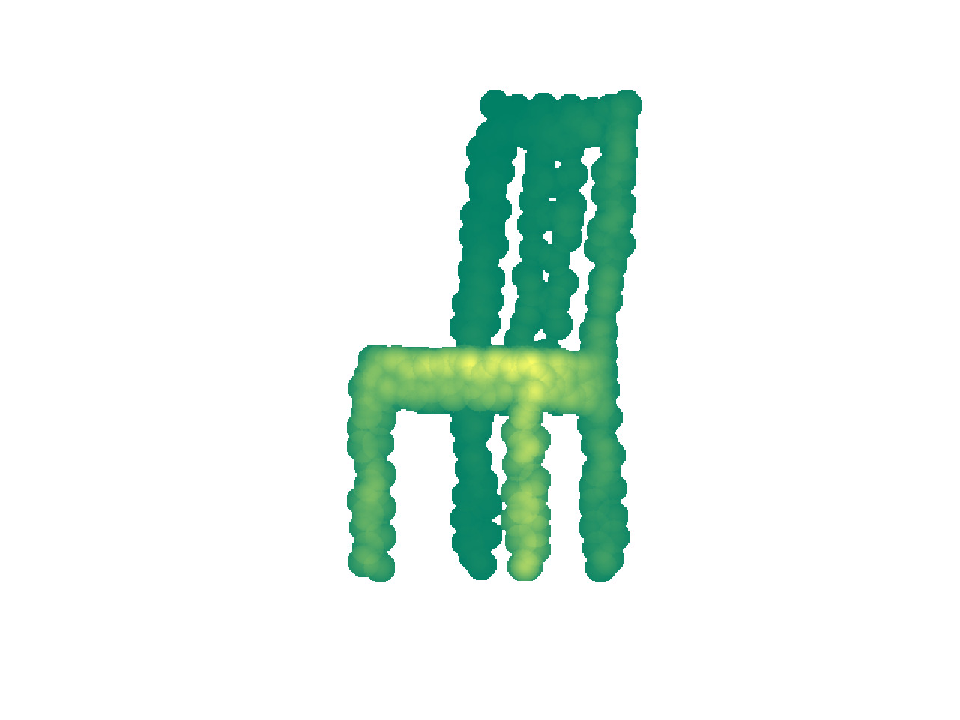
\includegraphics[trim=130 0 80 0,clip,width=0.15\textwidth]{chair_large-eps-converted-to.pdf}
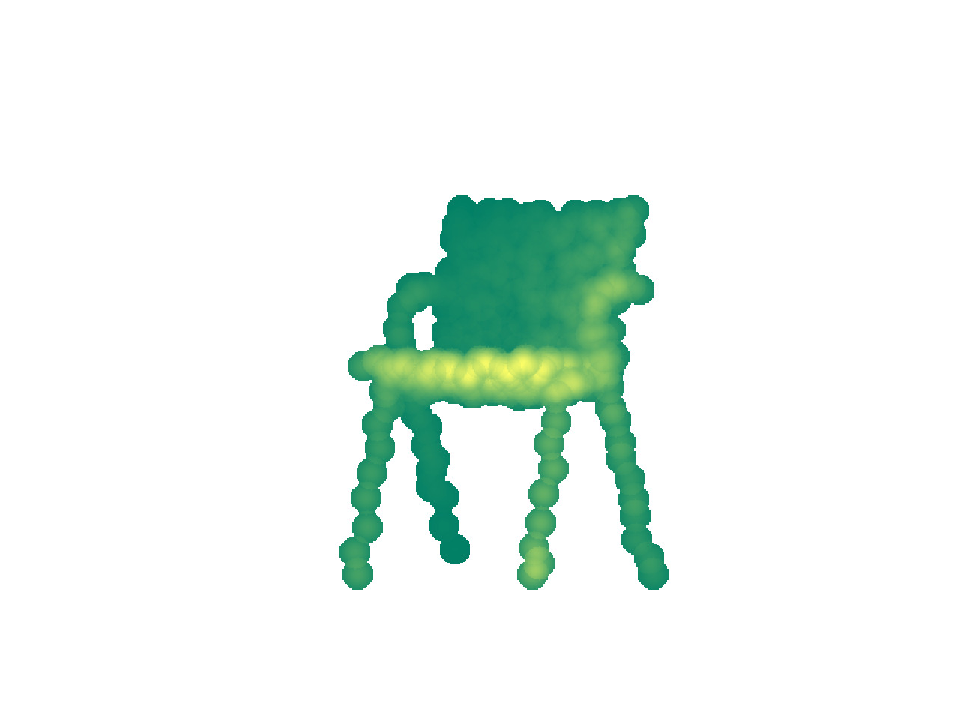
\includegraphics[trim=90 0 100 0,width=0.15\textwidth]{chair_large1-eps-converted-to.pdf}  
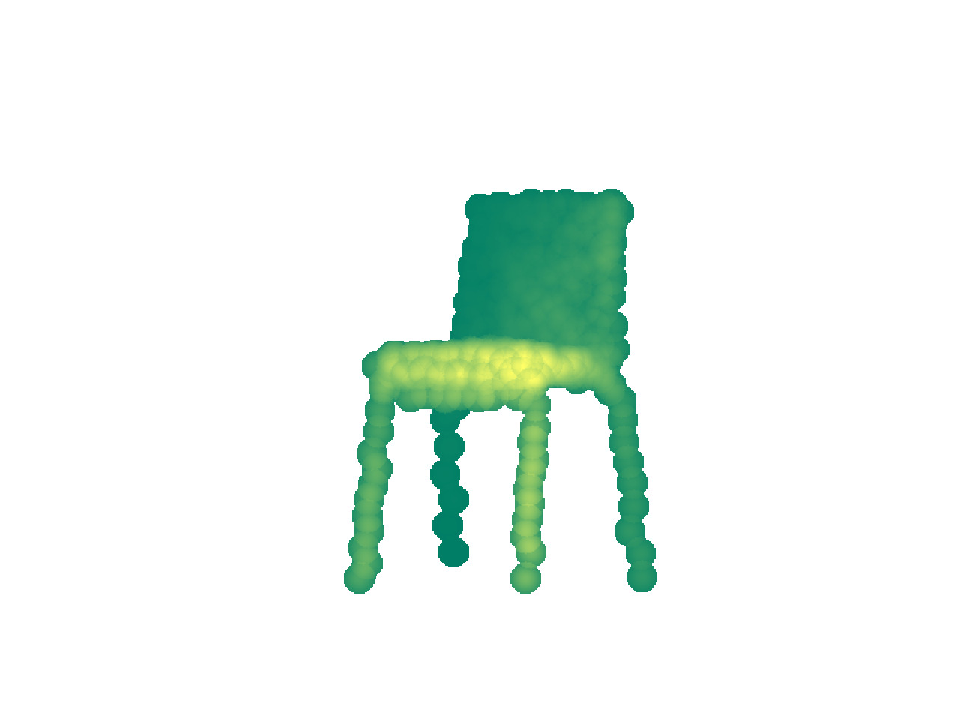
\includegraphics[trim=60 0 100 0,width=0.15\textwidth]{chair_large2-eps-converted-to.pdf} 
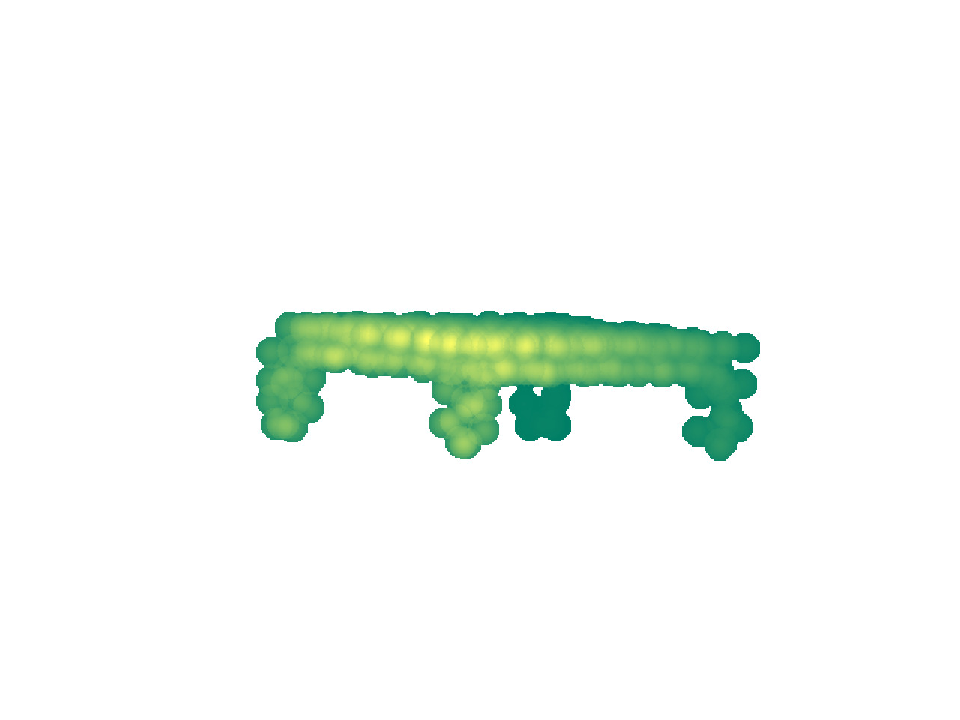
\includegraphics[trim=60 0 50 0,width=0.15\textwidth]{table_large-eps-converted-to.pdf}  
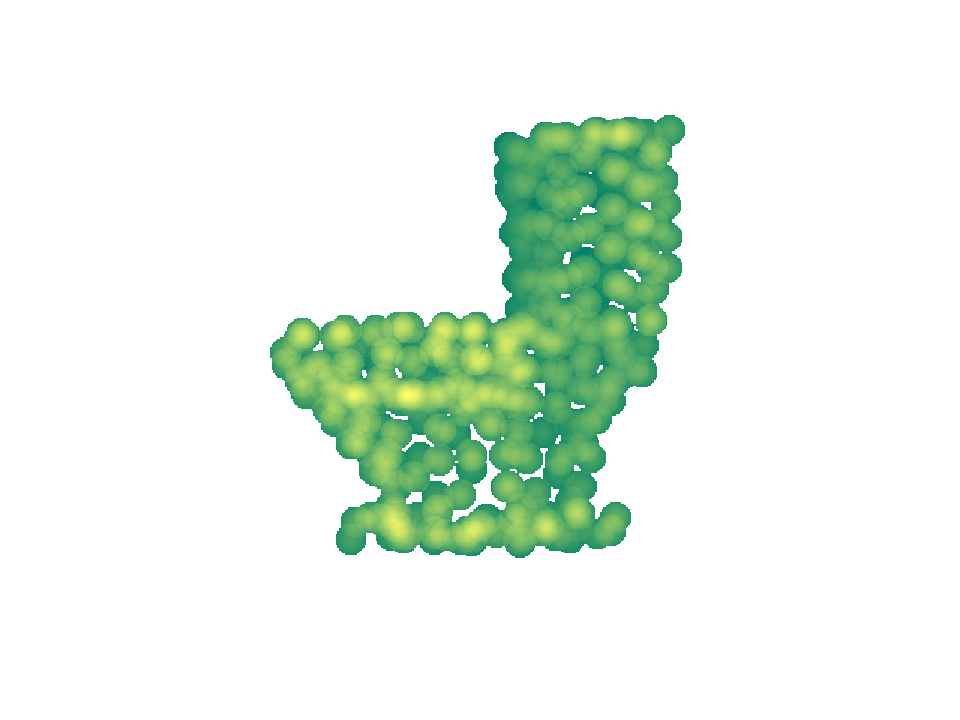
\includegraphics[trim=60 0 100 0,width=0.15\textwidth]{toilet_large-eps-converted-to.pdf}  
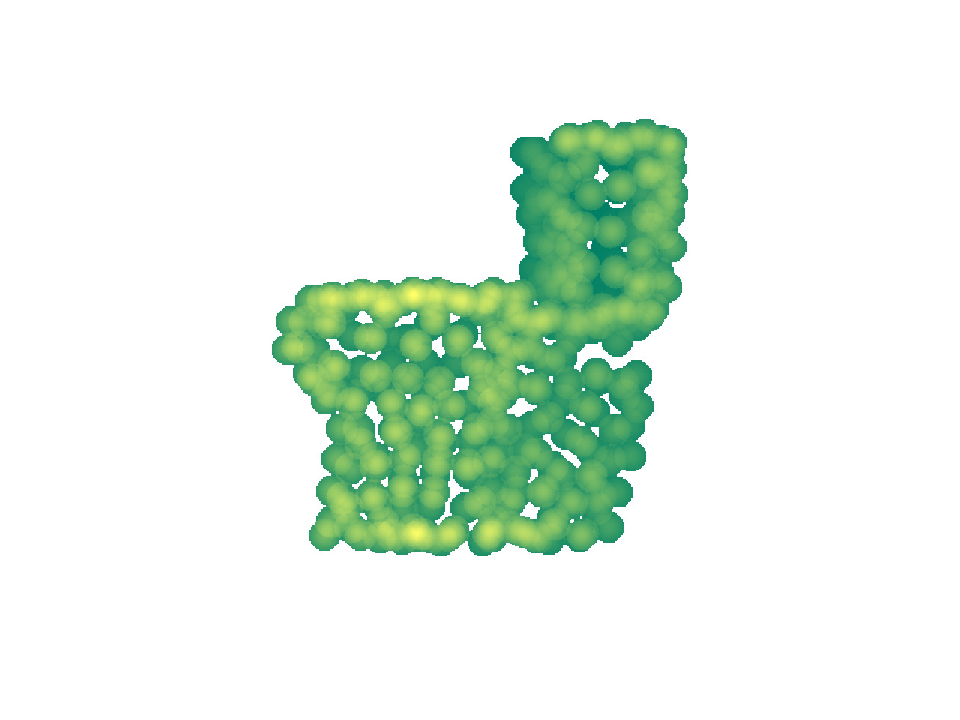
\includegraphics[trim=60 0 100 0,width=0.15\textwidth]{toilet_large1-eps-converted-to.pdf} 

\caption{Point cloud models with 300 sampling points in each model. Our goal is to identify chair models from other models such as toilet and table. }
\label{fig:points}
\end{figure*}

\myparagraph{Dataset} We evaluate our MNN stability results on the ModelNet10 \cite{wu20153d} classification problem. The dataset contains 3991 meshed CAD models from 10 categories for training and 908 models for testing. For each model, 300 points are uniformly randomly sampled from all points of the model to form the point cloud. Each point is characterized by the 3D coordinates as features. We formulate the problem by modeling a dense graph neural network model to approximate MNN. Each node in the graph can be modeled as the sampling point and each edge weight is constructed based on the distance between each pair of nodes.  In this work our goal is to identify the CAD model for chairs as is illustrated in Figure \ref{fig:points} with the models for chair labeled as 1 and the others as 0. We deform the underlying manifold structure by adding random perturbations to the coordinates of the sampling points. By comparing the differences of the classification error rates, we aim to show that MNNs with Lipschitz continuous and integral Lipschitz continuous manifold filters are stable via looking into the performance of the approximated GNNs. 

\myparagraph{Neural network architectures} We build dense graphs to approximate the point cloud models. We use the coordinates of each point as node features. By connecting a point with all the other points in the point cloud, the edge weight is defined based the distance between every two points and a Gaussian kernel. The Laplacian matrix is calculated for each input point cloud model. We implement different architectures, including Graph Filters (GF) and Graph Neural Networks (GNN) with 1 and 2 layers,  to solve the classification problem. The architectures with a single layer contain $F_0=3$ input features which are the 3d coordinates of each point, $F_1=64$ output features and $K=5$ filter taps. While the architectures with 2 layers has another layer with $F_2= 32$ features and $5$ filter taps. We use the ReLU as nonlinearity. The learned graph filters are not regularized in architectures with 'NoPel' while graph filters in the other architectures are both Lipschitz and integral Lipschitz. All architectures also include a linear readout layer mapping the final output features to a binary scalar that estimates the classification. 

\myparagraph{Discriminability experiment} We train all the architectures with an ADAM optimizer \cite{kingma2014adam} with learning rate set as 0.005 and decaying factors as 0.9, 0.999 by minimizing the entropy loss. The training point cloud models are divided in batches of 10 over 40 epochs. We run 5 random point samplings for all the architectures and we show the average classification error rates across these realizations as well as the standard deviation in Table \ref{tb:results}. We can observe that with the use of non-linearity, Graph Neural Networks perform better compared with Graph Filters. Architectures with more layers learn more accurate models which also leads to better performances.  

%%%%%%%%%%%%%%%%%%%%%%%%%%%%%%%%%%%%%%%%%%%%%%%%
%%%%%%%%%%%%%%%%%% TABLE %%%%%%%%%%%%%%%%%%%%%%% 
%%%%%%%%%%%%%%%%%%%%%%%%%%%%%%%%%%%%%%%%%%%%%%%%
\begin{table}[h]
\centering
\begin{tabular}{l|c} \hline
Architecture    & error rates   \\ \hline
GNN1Ly	& $8.04 \% \pm 0.88\% $   \\ \hline
GNN2Ly		& $4.30\% \pm 2.64\%$   \\ \hline
GF1Ly		& $13.77\% \pm 6.87\%$   \\ \hline
GF2Ly	& $12.22\% \pm 7.89\%$   \\ \hline
\end{tabular}
\caption{Classification error rates for model 'chair' in the test dataset. Average over 5 data realizations. The number of nodes is $N=300$.}
\label{tb:results}
\vspace{-3mm}
\end{table} 

\myparagraph{Stability experiment} We test the same trained Graph Neural Networks and Graph Filters with 2 layers on perturbed test point cloud models with different perturbation levels. We perturb the test point clouds by adding a Gaussian random variable with mean $\epsilon$ and variance $2\epsilon$ to each coordinate of every sampling point, which can be seen as a deformation of the underlying manifold. We measure the stability by computing the difference between the error rates achieved based on the original test point cloud models and the perturbed ones. In Figure \ref{fig:sim}, we see that this difference increases when the perturbations become larger, but overall the differences are small. We also observe that Graph Neural Network is more stable compared with Graph Filters. Furthermore, the Graph Neural Networks and Graph Filters with Lipschitz continuous and integral Lipschitz continuous filters are more stable. Both of these observations validate our stability results. 

%%%%%%%%%%%%%%%%%%%%%%%%%%%%%%%%%%%%%%%%%%%%%%%%
%%%%%%%%%%%%%%%%%% FIGURE %%%%%%%%%%%%%%%%%%%%%% 
%%%%%%%%%%%%%%%%%%%%%%%%%%%%%%%%%%%%%%%%%%%%%%%%
\begin{figure}[h]
  \centering
  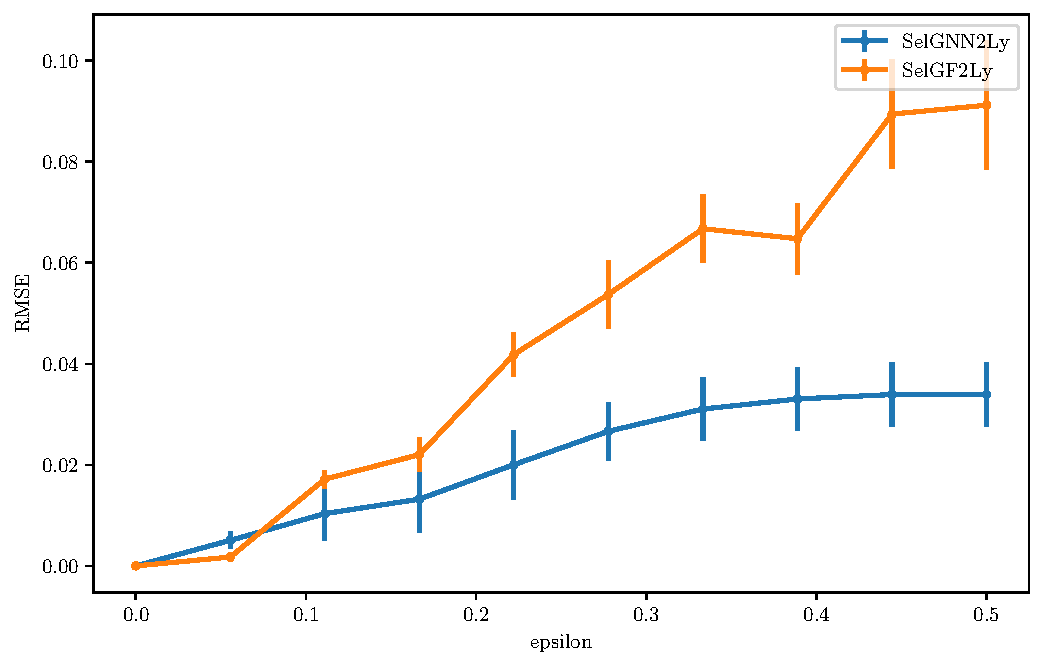
\includegraphics[height=4.5cm,width=6.5cm]{allCostTest.pdf}
\caption{Difference between error rates on the original test dataset and the deformed one. }
\label{fig:sim}
\end{figure}

%%%%%%%%%%%%%%%%%%%%%%%%%%%%%%%%%%%%%%%%%%%%%%%%
%%%%%%%%%%%%%%%%%% FIGURE %%%%%%%%%%%%%%%%%%%%%% 
%%%%%%%%%%%%%%%%%%%%%%%%%%%%%%%%%%%%%%%%%%%%%%%%
\begin{figure}[h]
  \centering
  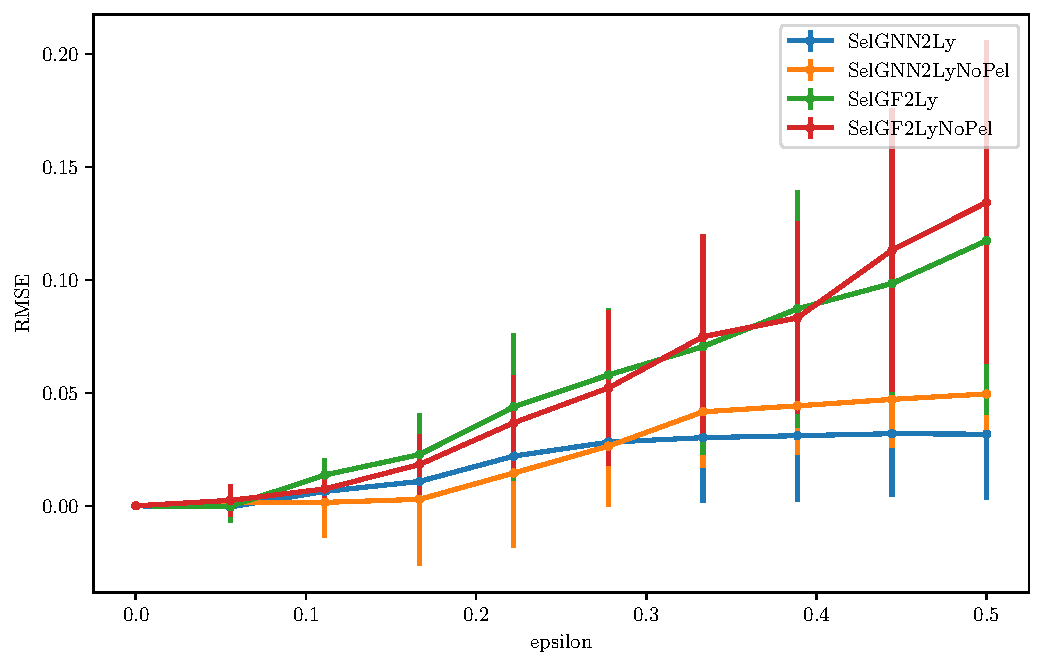
\includegraphics[height=4.5cm,width=6.5cm]{allCostTest_nopenalty.pdf}
\caption{Difference between error rates on the original test dataset and the deformed one. }
\label{fig:sim}
\end{figure}
To further verify the discriminability under perturbations, we trained and tested the architectures with perturbed dataset. We can see from Table \ref{tb:results-perturb} that both GNN and GF can identify the chair model with small error rates while the error rates grow slightly with the increase of perturbation levels. GNNs still outperform GFs in discriminablity with the help of nonlinearity.

%%%%%%%%%%%%%%%%%%%%%%%%%%%%%%%%%%%%%%%%%%%%%%%%
%%%%%%%%%%%%%%%%%% TABLE &&&&&%%%%%%%%%%%%%%%%%% 
%%%%%%%%%%%%%%%%%%%%%%%%%%%%%%%%%%%%%%%%%%%%%%%%
\begin{table}[h]
\centering
\begin{tabular}{l|c |c  } \hline
Architecture    & $\epsilon = 0.2$ & 0.4   \\ \hline
GNN2Ly		& $7.37\% \pm 1.43\%$ &  $7.71\% \pm 3.96\%$ \\\hline
GF2Ly	& $13.76\% \pm 6.82\%$  & $13.54\% \pm 7.16\%$  \\ \hline\hline
Architecture    & $\epsilon = 0.6$ & 0.8   \\ \hline
GNN2Ly& $8.04\% \pm 2.83\%$ & $11.01\% \pm 6.33\%$  \\ \hline
GF2Ly	& $14.76\% \pm 5.67\%$ & $16.04\% \pm 6.34\%$ \\ \hline
\end{tabular}
\caption{Classification error rates for model 'chair' with perturbed training and test dataset. Average over 5 data realizations. The number of nodes is $N=300$.}
\label{tb:results-perturb}
\vspace{-3mm}
\end{table} 

% We take GNNs as discretizations of MNNs to help verify our results. By constructing a graph model to represent the wireless adhoc network structure, we can solve the optimal resource allocation problem with a GNN. We consider a wireless adhoc network with $n=50$ pairs of transmitters and receivers within a range of $[-50m, 50m]^2$, i.e., the transmitter density is $\rho=0.02 \text{ transmitter}/m^2$. The receiver $r(i)$ is paired with the transmitter $i$ by dropping randomly around the transmitter. The channel link state between each transmitter and receiver is denoted  $[\bbS(t)]_{ij}:=s_{ij}(t)\in\reals_+$ at time $t$ between transmitter $i$ and receiver $r(j)$. %We measure the link condition by combining the large-scale pathloss gain and a random fast fading gain, which can be written as: $h_{ij}=\log(d_{ij}^{-2.2} h^f)$. The distance between transmitter $i$ and receiver $r(j)$ is denoted as $d_{ij}$ while $h^f\sim \text{Rayleigh}(2)$ stands for the fast fading gain. 
% Here, we focus on the power allocation problem among $n$ transmitters over an AWGN channel with interference, with $\bbp(\bbS)=[p_1(\bbS),p_2(\bbS),\hdots,p_n(\bbS)]$ denoting the power allocated to each transmitter under channel condition $\bbS$. The Shannon channel rate of transmitter $i$ is represented as $f_i$. The goal is to maximize the sum rate capacity under a total power budget $P_{max}$. The problem can be formulated as an optimization problem as
% \begin{align}
% %\label{eqn:prob_sim}
% f^* &=\max_{\bbp(\bbS)} \sum_{i=1}^n f_i \\
% s.t.\quad \nonumber &r_i=\mathbb{E}\left[  \log\left(1+\frac{s_{ii}^2 p_i(\bbS)}{1+ \sum\limits_{j\neq i}s_{ij}^2 p_j(\bbS)}\right) \right],\\
%   \nonumber & \mathbb{E}[\bm{1}^T\bbp]\leq P_{max},\quad p_i(\bbS)\in \{0,p_0\}.
% \end{align}
% With the transmitters and receivers modeled as graph nodes, the links between each transmitter and receiver can therefore be seen as edges. The channel matrix $\bbS$ composed of link conditions can be seen as the graph shift operator. 
% In the real world, the distribution of the transmitters can vary, which can be seen as a deformation to the underlying manifold. To capture this, we model the deformation by changing the density and the location distribution of the transmitters respectively. 

%  We measure policy performance in terms of the ratio of the sum-of-rate achieved by the GNN and a baseline heuristic method (WMMSE \cite{shi2011iteratively}) after training for 40,000 iterations (details on hyperparameters and other settings can be found in the appendices). We observe that the sum of capacity converges and the trained GNN can achieve the optimal power allocation policy on the original graph. By employing the same GNN (i.e., with the same parameters) on the deformed graph, we measure stability by computing the difference between the ratios achieved in the original wireless network setting and in the deformed settings described in the caption of Figure \ref{fig:sim}. In this figure, we see that this difference increases when the perturbations become larger, but overall the differences are small. We also compare GNNs with different architectures, and observe that deeper and wider GNNs are less stable. Both of these observations validate our stability results.

% \begin{figure}[t]
%   \centering
%   \subfloat[Stability to varying density. \label{fig:a}]{\includegraphics[height=4.5cm,width=6.5cm]{densityratio.eps}}\qquad
%   \subfloat[Stability to mixed uniform distributions. \label{fig:b}]{\includegraphics[height=4.5cm,width=6.5cm]{mixeduniformratio.eps}}
% \caption{Difference between the sum-of-rate ratios on the original wireless network setting and the deformed one. The $x$ axis in Figure \ref{fig:a} stands for the change on transmitter density, i.e., the perturbed density is given by $\rho'=\rho/(1-\sigma_1)$. In Figure \ref{fig:b}, the $x$-axis measures the perturbation to the original uniform distribution of the transmitters' locations. In the range $[-50m,0]$, a transmitter is dropped with probability $(1+\sigma_2)/2$, and in $[0, 50m]$, with probability $(1-\sigma_2)/2$ on each direction.}
% \label{fig:sim}
% \end{figure}

\section{Conclusions}
\label{sec:conclusion}
%!TEX root = stability_manifold_TSP.tex
In this paper, we have defined manifold convolutions and manifold neural networks. We prove that the deformations on the embedded submanifolds can be represented as a form of perturbations to the Laplace-Beltrami operator. Considering the infinite dimensionality of LB operators, we import the definition of frequency difference threshold filters and frequency ratio threshold filters to help separate the spectrum. By assigning similar frequency responses to the eigenvalues that are close enough, these filters can be proved to be stable under absolute and relative perturbations to the LB operator respectively with Lipschitz continuous assumptions. While the manifold filters need to trade-off between the stability and discriminability.  MNNs composed with layers of manifold filters and pointwise nonlinearities can be proved to be stable to absolute and relative perturbations to the LB operators. While the frequency mixing brought by pointwise nonlinearity can help with the discriminability. We conclude that the MNNs are thus both stable to deformations and discriminative. We also show the discretizations of MNNs in both spatial and time domains to make our proposed MNNs implementable. 
We finally verified our results numerically with a point cloud classification problem with ModelNet10 dataset.
%%%%%%%%%%%%%%%%%%%%%%%%%%%%%%%%%%%%%%%%%%%%%%%%%%%%%%%%%%%%



\urlstyle{same}
\bibliographystyle{IEEEtran}
\bibliography{references}




\appendix
 {\section{Appendix}
 version https://git-lfs.github.com/spec/v1
oid sha256:acf082414844baa070da9f4ef2b0d8ae3ee7cf1d71ef93bfb27903fab9bf8ac2
size 6711
}

\clearpage
\setcounter{page}{1}
\begin{center}
\textbf{\large Supplemental Materials}
\end{center}

\section{Supplementary Materials}
%%%%%%%%%%%%%%%%%%%%%%%%%%%%%%%%%%%%%%%%%%%%%%%%
%%%%%%%%%%%%%%%%%% SUBSECTION %%%%%%%%%%%%%%%%%% 
%%%%%%%%%%%%%%%%%%%%%%%%%%%%%%%%%%%%%%%%%%%%%%%%
\setcounter{subsection}{0}
\subsection{Proof of Proposition \ref{prop:finite_num}}
Weyl's law \cite[Chapter~1]{arendt2009mathematical} states that if $(\ccalM, g)$ is a compact Riemannian manifold of dimension $d$, then 
\begin{equation}\label{eqn:weylslaw}
\lambda_k = \frac{C_1}{C_d^{2/d}}\left(\frac{k}{Vol(\ccalM)} \right)^{2/d},
\end{equation}
where $C_d$ denotes the volume of the unit ball of $\reals^d$ and $C_1$ is an arbitrary constant. Therefore, if $\lambda_{k+1}-\lambda_k\leq \alpha$, we have
\begin{align}
    (k+1)^{2/d}-k^{2/d}\leq \frac{\alpha}{C_1} (Vol(\ccalM) C_d)^{2/d}
\end{align}
while the left side can be scaled down to $(k+1)^{2/d}-k^{2/d}\geq \frac{2}{d}k^{2/d-1}$. This implies that 
\begin{align}
    k^{\frac{2-d}{d}}\leq \left( \frac{\alpha d (Vol(\ccalM) C_d)^{2/d}}{2C_1} \right)^{\frac{d}{2-d}},
\end{align}
with $d>2$, we can claim that for 
$$k> \lceil (\alpha d/C_1)^{d/(2-d)}(C_d \text{Vol}(\ccalM))^{2/(2-d)} \rceil,$$ it holds that $\lambda_{k+1}-\lambda_k\leq \alpha$. Proof of Proposition \ref{prop:finite_num_rela} is similar and is also based on \eqref{eqn:weylslaw}.
\subsection{Proof of Theorem \ref{thm:stability_rela_filter}}
\label{app:stability_rela_filter}
The decomposition follows the same routine as \eqref{eqn:diff} shows. 
By decomposing the filter function as \eqref{eqn:h0-gamma} and \eqref{eqn:hl-gamma}, the norm difference can also be bounded separately. 
\begin{align}
\label{eqn:h0-gamma}& h^{(0)}(\lambda) = \left\{ 
\begin{array}{cc} 
                \hat{h}(\lambda)-\sum\limits_{l\in\ccalK_m}\hat{h}(C_l)  &  \lambda\in[\Lambda_k(\gamma)]_{k\in\ccalK_s} \\
                0& \text{otherwise}  \\
                \end{array} \right.  \\
\label{eqn:hl-gamma}& h^{(l)}(\lambda) = \left\{ 
\begin{array}{cc} 
                \hat{h}(C_l) &  \lambda\in[\Lambda_k(\gamma)]_{k\in\ccalK_s} \\
                \hat{h}(\lambda) & 
                \lambda\in\Lambda_l(\gamma)\\
                0 &
                \text{otherwise}  \\
                \end{array} \right.             
\end{align}
where now $\hat{h}(\lambda)=h^{(0)}(\lambda)+\sum_{l\in\ccalK_m}h^{(l)}(\lambda)$ with $\ccalK_s$ defined as the group index set of singletons and $\ccalK_m$ the set of partitions that contain multiple eigenvalues. For manifold filter $\bbh^{(0)}(\ccalL)$ with filter function $h^{(0)}(\lambda)$, the norm difference can also be written as
\begin{align}
 \label{eqn:rela-h0}  & \nonumber \left\| \sum_{i=1}^\infty h^{(0)}(\lambda_{i}) \langle f, \bm\phi_i \rangle \bm\phi_i  -  h^{(0)}(\lambda'_i )  \langle f, \bm\phi'_i \rangle \bm\phi'_i \right\| \\
  & \nonumber \leq \left\| \sum_{i=1}^\infty h^{(0)}(\lambda_i )\langle f, \bm\phi_i \rangle (\bm\phi_i - \bm\phi'_i ) \right\| \\ \nonumber&\qquad\qquad  + \Bigg\|  \sum_{i =1}^\infty  h^{(0)}(\lambda_i )\langle f, \bm\phi_i - \bm\phi'_i  \rangle \bm\phi'_i \Bigg\|\\& \qquad\qquad \quad+ \left\|\sum_{i=1}^\infty  (h^{(0)}(\lambda_i ) -h^{(0)}(\lambda'_i) ) \langle f, \bm\phi'_i \rangle \bm\phi'_i  \right\| . 
\end{align}
The difference of the eigenvalues due to relative perturbations can be similarly addressed by Lemma \ref{lem:eigenvalue_relative}.


The first two terms of \eqref{eqn:rela-h0} rely on the differences of eigenfunctions, which can be derived with Davis-Kahan Theorem in Lemma \ref{lem:davis-kahan}, the difference of eigenfunctions can be written as
\begin{align}
\| \ccalE\ccalL \bm\phi_i \| =\| \ccalE\lambda_i\bm\phi_i \|=\lambda_i \|\ccalE \bm\phi_i\|\leq\lambda_i\|\ccalE\|\|\bm\phi_i\|\leq \lambda_i \epsilon.
\end{align}
The first term in \eqref{eqn:rela-h0} then can be bounded as
\begin{align}
&\nonumber\left\| \sum_{i=1}^\infty h^{(0)}(\lambda_i )\langle f, \bm\phi_i \rangle (\bm\phi_i - \bm\phi'_i ) \right\|\\
& \leq \sum_{i=1}^\infty |h^{(0)}(\lambda_i)| | \langle f, \bm\phi_i \rangle | \left\|\bm\phi_i-\bm\phi'_i \right\| \leq \sum_{i\in\ccalK_s} \frac{\pi\lambda_i \epsilon}{2d_i}  \|f\|.
\end{align} 
Because $d_i=\min\{ |\lambda_i-\lambda'_{i-1}|, |\lambda'_i-\lambda_{i-1}|, |\lambda'_{i+1}-\lambda_i| , | \lambda_{i+1}-\lambda'_i|\}$, with Lemma \ref{lem:eigenvalue_relative} implied, we have
\begin{gather}
|\lambda_i-\lambda'_{i-1}|\geq | \lambda_i - (1+\epsilon)\lambda_{i-1}|,\\
 |\lambda'_i-\lambda_{i-1}|\geq |(1-\epsilon)\lambda_i-\lambda_{i-1}|,\\ |\lambda'_{i+1}-\lambda_i|\geq | (1-\epsilon)\lambda_{i+1}-\lambda_i|,\\| \lambda_{i+1}-\lambda'_i|\geq |\lambda_{i+1}-(1+\epsilon)\lambda_i|.
\end{gather}
Combine with Lemma \ref{lem:eigenvalue_relative} and Definition \ref{def:frt-spectrum}, $d_i\geq \epsilon\gamma +\gamma-\epsilon$:
\begin{align}
 |(1-\epsilon)\lambda_{i+1}-\lambda_i|
 &\geq |\gamma \lambda_i-\epsilon \lambda_{i+1}|\\
 &=\epsilon \lambda_i\left|1-\frac{\lambda_{i+1}}{\lambda_i}+\frac{\gamma}{\epsilon}-1\right|\\&\geq \lambda_i(\gamma-\epsilon+\gamma\epsilon)
\end{align}
This leads to the bound as
\begin{align}
\left\| \sum_{i=1}^\infty h^{(0)}(\lambda_i )\langle f, \bm\phi_i \rangle (\bm\phi_i - \bm\phi'_i ) \right\| \leq   \frac{M_s \pi \epsilon}{2(\gamma-\epsilon+\gamma\epsilon)} \|f\|.
\end{align}

The second term in \eqref{eqn:rela-h0} can also be bounded as
\begin{align}
    &\nonumber \left\|  \sum_{i =1}^\infty  h^{(0)}(\lambda_i )\langle f, \bm\phi_i - \bm\phi'_i  \rangle \bm\phi'_i \right\| \\
 &\leq   \sum_{i =1}^\infty |h^{(0)}(\lambda_i)| \|\bm\phi_i - \bm\phi'_i \| \|f\|  \leq   \frac{M_s \pi \epsilon}{2(\gamma-\epsilon+\gamma\epsilon)} \|f\|,
\end{align}
which similarly results from the fact that $|h^{(0)}(\lambda)|<1$ and $h^{(0)}(\lambda)=0$ for $\lambda\in[\Lambda_k(\gamma)]_{k\in\ccalK_m}$. The number of eigenvalues within $[\Lambda_k(\gamma)]_{k\in\ccalK_s}$ is denoted as $M_s$.

The third term in \eqref{eqn:rela-h0} is:
\begin{align}
   &\nonumber \Bigg\|\sum_{i=1}^\infty  (h^{(0)}(\lambda_i ) -h^{(0)}(\lambda'_i) ) \langle f, \bm\phi'_i \rangle \bm\phi'_i  \Bigg\|^2 \\
    &\leq  \sum_{i=1}^\infty\left( \frac{B_h \epsilon|\lambda_i|}{(\lambda_i+\lambda_i')/2}\right)^2   \langle f,\bm\phi'_i \rangle^2 \leq \left( \frac{2B_h\epsilon}{2-\epsilon}\right)^2\|f\|^2,
\end{align}
with the use of Lemma \ref{lem:eigenvalue_relative} and Definition \ref{def:int-lipschitz}.

Then we need to analyze the output difference of $h^{(l)}(\lambda)$.
\begin{align}
     \nonumber &\left\| \bbh^{(l)}(\ccalL)f -\bbh^{(l)}(\ccalL')f \right\| 
    \\& \leq \left\| (\hat{h}(C_l)+\delta)f -(\hat{h}(C_l)-\delta)f\right\| \leq 2\delta\|f\|.
\end{align}

Combine the filter function, we could get 
\begin{align}
\label{eqn:sta-filter-gamma}
    \nonumber &\|\bbh(\ccalL)f-\bbh(\ccalL')f\|=\\&
    \left\|\bbh^{(0)}(\ccalL)f +\sum_{l\in\ccalK_m}\bbh^{(l)}(\ccalL)f - \bbh^{(0)}(\ccalL')f - \sum_{l\in\ccalK_m} \bbh^{(l)}(\ccalL')f \right\|\\
    &\leq \|\bbh^{(0)}(\ccalL)f-\bbh^{(0)}(\ccalL')f\|+\sum_{l\in\ccalK_m}\|\bbh^{(l)}(\ccalL)f-\bbh^{(l)}(\ccalL')f\|\\
    &\leq \frac{M_s\pi\epsilon}{\gamma-\epsilon+\gamma\epsilon}\|f\| + \frac{2B_h\epsilon}{2-\epsilon}\|f\| +2(M-M_s)\delta\|f\|,
\end{align}
which concludes the proof.


%%%%%%%%%%%%%%%%%%%%%%%%%%%%%%%%%%%%%%%%%%%%%%%%
%%%%%%%%%%%%%%%%%% SUBSECTION %%%%%%%%%%%%%%%%%% 
%%%%%%%%%%%%%%%%%%%%%%%%%%%%%%%%%%%%%%%%%%%%%%%%
\setcounter{subsection}{1}
\subsection{Proof of Theorem \ref{thm:stability_nn}}
\label{app:stability_nn}
To bound the output difference of MNNs, we need to write in the form of features of the final layer
 \begin{equation}
 \|\bm\Phi(\bbH,\ccalL,f)-\bm\Phi(\bbH,\ccalL',f)\| =  \left\| \sum_{q=1}^{F_L} f_L^q - \sum_{q=1}^{F_L} f_L^{'q}\right\|.
 \end{equation}
The output signal of layer $l$ of MNN $\bbPhi(\bbH,\ccalL, f)$ can be written as
\begin{equation}
 f_l^p = \sigma\left( \sum_{q=1}^{F_{l-1}} \bbh_l^{pq}(\ccalL) f_{l-1}^q\right).
\end{equation}
Similarly, for the perturbed $\ccalL'$ the corresponding MNN is $\bbPhi(\bbH,\ccalL',f)$ the output signal can be written as
 \begin{equation}
 f_l^{'p} = \sigma\left( \sum_{q=1}^{F_{l-1}} \bbh_l^{pq}(\ccalL') f_{l-1}^{'q}\right).
 \end{equation}
The difference therefore becomes
 \begin{align}
 &\nonumber\| f_l^p - f_l^{'p} \| \\& =\left\|  \sigma\left( \sum_{q=1}^{F_{l-1}} \bbh_l^{pq}(\ccalL) f_{l-1}^q\right) -  \sigma\left( \sum_{q=1}^{F_{l-1}} \bbh_l^{pq}(\ccalL') f_{l-1}^{'q}\right) \right\|.   
 \end{align}
With the assumption that $\sigma$ is normalized Lipschitz, we have
 \begin{align}
  \| f_l^p - f_l^{'p} \| &\leq \left\| \sum_{q=1}^{F_{l-1}}  \bbh_l^{pq}(\ccalL) f_{l-1}^q - \bbh_l^{pq}(\ccalL') f_{l-1}^{'q}  \right\| \\&\leq \sum_{q=1}^{F_{l-1}} \left\|  \bbh_l^{pq}(\ccalL) f_{l-1}^q - \bbh_l^{pq}(\ccalL') f_{l-1}^{'q} \right\|.
 \end{align}
By adding and subtracting $\bbh_l^{pq}(\ccalL') f_{l-1}^{q}$ from each term, combined with the triangle inequality we can get
 \begin{align}
 & \nonumber \left\|  \bbh_l^{pq}(\ccalL) f_{l-1}^q - \bbh_l^{pq}(\ccalL') f_{l-1}^{'q} \right\| \\\nonumber &\quad \leq \left\|  \bbh_l^{pq}(\ccalL) f_{l-1}^q - \bbh_l^{pq}(\ccalL') f_{l-1}^{q} \right\| \\&\qquad \qquad \qquad + \left\| \bbh_l^{pq}(\ccalL') f_{l-1}^q - \bbh_l^{pq}(\ccalL') f_{l-1}^{'q} \right\|
 \end{align}
The first term can be bounded with \eqref{eqn:sta-filter-alpha} for absolute perturbations. The second term can be decomposed by Cauchy-Schwartz inequality and non-amplifying of the filter functions as
 \begin{align}
 \left\| f_{l}^p - f_l^{'p} \right\| \leq \sum_{q=1}^{F_{l-1}} C_{per} \epsilon \| f_{l-1}^q\| + \sum_{q=1}^{F_{l-1}} \| f_{l-1}^q - f_{l-1}^{'q} \|,
 \end{align}
where $C_{per}$ representing the constant in the stability bound of manifold filters. To solve this recursion, we need to compute the bound for $\|f_l^p\|$. By normalized Lipschitz continuity of $\sigma$ and the fact that $\sigma(0)=0$, we can get
 \begin{align}
 \nonumber &\| f_l^p \|\leq \left\| \sum_{q=1}^{F_{l-1}} \bbh_l^{pq}(\ccalL) f_{l-1}^{q}  \right\| \leq  \sum_{q=1}^{F_{l-1}}  \left\| \bbh_l^{pq}(\ccalL)\right\|  \|f_{l-1}^{q}  \| \\
 &\qquad \leq   \sum_{q=1}^{F_{l-1}}   \|f_{l-1}^{q}  \| \leq \prod\limits_{l'=1}^{l-1} F_{l'} \sum_{q=1}^{F_0}\| f^q \|.
 \end{align}
 Insert this conclusion back to solve the recursion, we can get
 \begin{align}
 \left\| f_{l}^p - f_l^{'p} \right\| \leq l C_{per}\epsilon \left( \prod\limits_{l'=1}^{l-1} F_{l'} \right) \sum_{q=1}^{F_0} \|f^q\|.
 \end{align}
 Replace $l$ with $L$ we can obtain
 \begin{align}
 &\nonumber \|\bm\Phi(\bbH,\ccalL,f) - \bm\Phi(\bbH,\ccalL',f)\| \\
 &\qquad \qquad \leq \sum_{q=1}^{F_L} \left( L C_{per}\epsilon \left( \prod\limits_{l'=1}^{L-1} F_{l'} \right) \sum_{q=1}^{F_0} \|f^q\| \right).
 \end{align}
 With $F_0=F_L=1$ and $F_l=F$ for $1\leq l\leq L-1$, then we have
  \begin{align}
 \|\bm\Phi(\bbH,\ccalL,f) - \bm\Phi(\bbH,\ccalL',f)\| \leq LF^{L-1} C_{per}\epsilon \|f\|,
 \end{align}
which concludes the proof.
 
 
 %%%%%%%%%%%%%%%%%%%%%%%%%%%%%%%%%%%%%%%%%%%%%%%%
%%%%%%%%%%%%%%%%%% SUBSECTION %%%%%%%%%%%%%%%%%% 
%%%%%%%%%%%%%%%%%%%%%%%%%%%%%%%%%%%%%%%%%%%%%%%%
%  \subsection{Proof of Theorem \ref{thm:stability_nn_rela}}
%  \label{app:stability_nn_rela}
%  For the stability of MNN with $\gamma$-FRT filters, the result can be derived with the same routine but replace the $C_{per}$ term as $C_{per}= \frac{M_s\pi}{\gamma-\epsilon+\gamma\epsilon}+\frac{2B_h}{2-\epsilon}+\frac{2(M-M_s)\delta}{\epsilon}$.
\setcounter{subsection}{2}
\subsection{Lemmas and Propositions}

Now we need to include two important lemmas to analyze the influence on eigenvalues and eigenfunctions caused by the perturbation.
\begin{lemma}\label{lem:eigenvalue_absolute}[Weyl's Theorem]
The eigenvalues of LB operators $\ccalL$ and perturbed $\ccalL'=\ccalL+\bbA$ satisfy
\begin{equation}
|\lambda_i-\lambda'_i|\leq \|\bbA\|, \text{ for all }i=1,2\hdots
\end{equation}
\end{lemma}
\begin{proof}[Proof of Lemma \ref{lem:eigenvalue_absolute}]

The minimax principle asserts that
\begin{align}
    \lambda_i(\ccalL)=\max_{codim T = i-1}\lambda[\ccalL, T]=\max_{codim T \leq i-1} \min_{u\in T, \|u\|=1} \langle \ccalL u, u \rangle.
\end{align}

Then for any $1\leq i $, we have
\begin{align}
    \lambda_i(\ccalL') &=\max_{codim T\leq i-1} \min_{ u\in T, \|u\|=1}  \langle (\ccalL+\bbA) u, u\rangle \\
    & = \max_{codim T\leq i-1} \min_{ u\in T, \|u\|=1} \left( \langle  (\ccalL  u, u\rangle + \langle \bbA u, u\rangle   \right)\\
    & \geq \max_{codim T\leq i-1} \min_{  u\in T, \|u\|=1}  \left\langle  \ccalL  u, u\rangle   + \lambda_1(\bbA) \right)\\
    & = \lambda_1(\bbA)+ \max_{codim T\leq i-1} \min_{  u\in T, \|u\|=1 } \langle  \ccalL  u, u\rangle  \\
    & = \lambda_i(\ccalL)+\lambda_1(\bbA).
\end{align}
Similarly, we can have $\lambda_i(\ccalL') \leq \lambda_i(\ccalL)+ \max_k\lambda_k(\bbA)$. This leads to $\lambda_1(\bbA)\leq \lambda_i(\ccalL' )-\lambda_i(\ccalL) \leq \max_k\lambda_k(\bbA)$. This leads to the conclusion that:
\begin{equation}
    |\lambda'_i-\lambda_i|\leq \|\bbA\|.
\end{equation}
\end{proof}

To measure the difference of eigenfunctions, we introduce the Davis-Kahan $\sin\theta$ theorem as follows.
\begin{lemma}[Davis-Kahan $\sin\theta$ Theorem]\label{lem:davis-kahan}
Suppose the spectra of operators $\ccalL$ and $\ccalL'$ are partitioned as $\sigma\bigcup\Sigma$ and $\omega\bigcup \Omega$ respectively, with $\sigma\bigcap \Sigma=\emptyset$ and $\omega\bigcap\Omega=\emptyset$. Then we have
\begin{equation}
\|E_\ccalL(\sigma)-E_{\ccalL'}(\omega)\|\leq \frac{\pi}{2}\frac{\|(\ccalL'-\ccalL)E_\ccalL(\sigma)\|}{d}\leq \frac{\pi}{2}\frac{\|\ccalL'-\ccalL\|}{d},
\end{equation}
where $d$ satisfies $\min_{x\in\sigma,y\in\Omega}|x-y|\geq d$ and $\min_{x\in\Sigma,y\in\omega}|x-y|\geq d$.
\end{lemma}
\begin{proof}[Proof of Lemma \ref{lem:davis-kahan}] 
See \cite{seelmann2014notes}.
\end{proof}


\begin{lemma}\label{lem:eigenvalue_relative}
The eigenvalues of LB operators $\ccalL$ and perturbed $\ccalL'=\ccalL+\ccalE\ccalL$ with $\|\ccalE\|= \epsilon$ satisfy
\begin{align}
    |\lambda_i-\lambda'_i|\leq \epsilon |\lambda_i|, \text{ for all }i=1,2\hdots
\end{align}
\end{lemma}
\begin{proof}[Proof of Lemma \ref{lem:eigenvalue_relative}]
With the assumption that $\ccalL'=\ccalL+\ccalE\ccalL$, we have
\begin{align}
    \lambda_i(\ccalL + \ccalE\ccalL)& = \max_{codim T\leq i-1} \min_{ u\in T, \|u\|=1}  \langle (\ccalL+\ccalE\ccalL) u, u\rangle \\
    & = \max_{codim T\leq i-1} \min_{u\in T, \|u\|=1} \left(  \langle \ccalL u, u\rangle   +  \langle \ccalE\ccalL u, u\rangle  \right)\\
    & =\lambda_i(\ccalL) + \max_{codim T\leq i-1} \min_{u\in T, \|u\|=1} \langle \ccalE\ccalL u, u\rangle.
\end{align}
For the second term, we have
\begin{align}
    |\langle \ccalE\ccalL u, u\rangle| &\leq \langle |\ccalE|  |\ccalL|u, u \rangle   \leq \epsilon \sum_i |\lambda_i(\ccalL)||\xi_i|^2 = \epsilon \langle |\ccalL| u,u \rangle
\end{align}
Therefore, we have
\begin{align}
 & \nonumber \lambda_i(\ccalL+\ccalE\ccalL) \leq \lambda_i(\ccalL) + \epsilon
   \max_{codim T\leq i-1} \min_{u\in T, \|u\|=1} \langle |\ccalL| u, u\rangle\\
   &\qquad \qquad\quad  = \lambda_i(\ccalL) + \epsilon |\lambda_i(\ccalL)|,\\
   &\lambda_i(\ccalL + \ccalE\ccalL) \geq \lambda_i(\ccalL) -\epsilon |\lambda_i(\ccalL)|,\\
   &\lambda_i(\ccalL)-\epsilon |\lambda_i(\ccalL)|\leq  \lambda_i(\ccalL + \ccalE\ccalL)\leq \lambda_i(\ccalL) +\epsilon|\lambda_i(\ccalL)|,
\end{align}
which concludes the proof.
\end{proof}
%%%%%%%%%%%%%%%%%%%%%%%%%%%%%%%%%%%%%%%%%%%%%%%%
%%%%%%%%%%%%%%%%%% SUBSECTION %%%%%%%%%%%%%%%%%% 
%%%%%%%%%%%%%%%%%%%%%%%%%%%%%%%%%%%%%%%%%%%%%%%% 
\setcounter{subsection}{3}

%%%%%%%%%%%%%%%%%%%%%%%%%%%%%%%%%%%%%%%%%%%%%%%%
%%%%%%%%%%%%%%%%%% SUBSECTION %%%%%%%%%%%%%%%%%% 
%%%%%%%%%%%%%%%%%%%%%%%%%%%%%%%%%%%%%%%%%%%%%%%% 
 \subsection{Proof of Proposition \ref{prop:convergence}}
 \label{app:convergence}
 Considering that the discrete points $\{x_1,x_2,\hdots,x_n\}$ are uniformly sampled from manifold $\ccalM$ with measure $\mu$, the empirical measure associated with $\text{d}\mu$ can be denoted as $p_n=\frac{1}{n}\sum_{i=1}^n \delta_{x_i}$, where $\delta_{x_i}$ is the Dirac measure supported on $x_i$. Similar to the inner product defined in the $L^2(\ccalM)$ space \eqref{eqn:innerproduct}, the inner product on $L^2(\bbG_n)$ is denoted as
 \begin{equation}
     \langle u, v\rangle_{L^2(\bbG_n)}=\int u(x)v(x)\text{d}p_n=\frac{1}{n}\sum_{i=1}^n u(x_i)v(x_i).
 \end{equation}
 The norm in $L^2(\bbG_n)$ is therefore $\|u\|^2_{L^2(\bbG_n)} = \langle u, u \rangle_{L^2(\bbG_n)}$, with $u,v \in L^2(\ccalM)$. For signals $\bbu,\bbv \in L^2(\bbG_n)$, the inner product is therefore $\langle \bbu,\bbv \rangle_{L^2(\bbG_n)} = \frac{1}{n}\sum_{i=1}^n [\bbu]_i[\bbv]_i$.
 
 We first import the existing results from \cite{belkin2006convergence} which indicates the spectral convergence of the constructed Laplacian operator based on the graph $\bbG_n$ to the LB operator of the underlying manifold.
 \begin{theorem}[Theorem 2.1 \cite{belkin2006convergence}]
 \label{thm:convergence}
 Let $X=\{x_1, x_2,...x_n\}$ be a set of $n$ points sampled i.i.d. from a $d$-dimensional manifold $\ccalM \subset \reals^N$. % sampled by an operator $\bbP_n$ \eqref{eqn:sampling}. 
 Let $\bbG_n$ be a graph approximation of $\ccalM$ constructed from $X$ with weight values set as \eqref{eqn:weight} with $t_n = n^{-1/(d+2+\alpha)}$ and $\alpha>0$. Let $\bbL_n$ be the graph Laplacian of $\bbG_n$ and $\ccalL$ be the Laplace-Beltrami operator of $\ccalM$. Let $\lambda_{i}^n$ be the $i$-th eigenvalue of $\bbL_n$ and $\bm\phi_{i}^n$ be the corresponding normalized eigenfunction. Let $\lambda_i$ and $\bm\phi_i$ be the corresponding eigenvalue and eigenfunction of $\ccalL$ respectively. Then, it holds that
\begin{equation}
\label{eqn:convergence_spectrum}
    \lim_{n\rightarrow \infty } \lambda_i^n = \lambda_i, \quad \lim_{n\rightarrow \infty} |\bm\phi^{n}_i(x_j) -  \bm\phi_i(x_j)|=0, j=1,2 \hdots,n
\end{equation}
where the limits are taken in probability.
 \end{theorem}
 

With the definitions of neural networks on graph $\bbG_n$ and manifold $\ccalM$, the output difference can be written as 
 \begin{align}
    \nonumber \|\bm\Phi(\bbH,\bbL_n,\bbP_nf)-\bbP_n \bm\Phi&(\bbH,\ccalL, f))\| = \left\| \sum_{q=1}^{F_L}\bbx_L^q-\sum_{q=1}^{F_L}\bbP_n f_L^q \right\|\\
     & \leq \sum_{q=1}^{F_L} \left\| \bbx_L^q- \bbP_n f_L^q \right\|.
 \end{align}
 By inserting the definitions, we have 
 \begin{align}
   \nonumber  &\left\| \bbx_l^p- \bbP_n f_l^p \right\|\\
     &=\left\| \sigma\left(\sum_{q=1}^{F_{l-1}} \bbh_l^{pq}(\bbL_n) \bbx_{l-1}^q \right) -\bbP_n \sigma\left(\sum_{q=1}^{F_{l-1}} \bbh_l^{pq}(\ccalL) f_{l-1}^q\right) \right\|
 \end{align}
 with $\bbx_0=\bbP_n f$ as the input of the first layer. With a normalized Lipschitz nonlinearity, we have
  \begin{align}
    \| \bbx_l^p - \bbP_n f_l^p & \| \leq \left\|  \sum_{q=1}^{F_{l-1}} \bbh_l^{pq}(\bbL_n) \bbx_{l-1}^q    - \bbP_n \sum_{q=1}^{F_{l-1}} \bbh_l^{pq}(\ccalL)  f_{l-1}^q\right\|\\
    & \leq \sum_{q=1}^{F_{l-1}} \left\|    \bbh_l^{pq}(\bbL_n) \bbx_{l-1}^q    - \bbP_n   \bbh_l^{pq}(\ccalL)  f_{l-1}^q\right\|
 \end{align}
 The difference can be further decomposed as
\begin{align}
   \nonumber   \|    \bbh_l^{pq}(\bbL_n) & \bbx_{l-1}^q    - \bbP_n   \bbh_l^{pq}(\ccalL)  f_{l-1}^q \| 
   \\ \nonumber&\leq \|
\bbh_l^{pq}(\bbL_n) \bbx_{l-1}^q  - \bbh_l^{pq}(\bbL_n) \bbP_n f_{l-1}^q \\ &\qquad +\bbh_l^{pq}(\bbL_n) \bbP_n f_{l-1}^q  - \bbP_n   \bbh_l^{pq}(\ccalL)  f_{l-1}^q
    \|\\\nonumber
   & \leq \left\|
    \bbh_l^{pq}(\bbL_n) \bbx_{l-1}^q  - \bbh_l^{pq}(\bbL_n) \bbP_n f_{l-1}^q
    \right\|
  \\ &\qquad +
    \left\|
    \bbh_l^{pq}(\bbL_n) \bbP_n f_{l-1}^q  - \bbP_n   \bbh_l^{pq}(\ccalL)  f_{l-1}^q
    \right\|
\end{align}
The first term can be bounded as $\| \bbx_{l-1}^q - \bbP_nf_{l-1}^q\|$ with the initial condition $\|\bbx_0 - \bbP_n f_0\|=0$. The second term can be denoted as $D_{l-1}^n$. With the iteration employed, we can have
\begin{align}
 \nonumber \|\bm\Phi(\bbH,\bbL_n,\bbP_n f) - \bbP_n \bm\Phi(\bbH,\ccalL,f)\| 
 \leq
 \sum_{l=0}^L \prod\limits_{l'=l}^L F_{l'} D_l^n.
 \end{align}
 Therefore, we can focus on the difference term $D_l^n$, we omit the feature and layer index to work on a general form.
  \begin{align}
    &\nonumber \|\bbh(\bbL_n)\bbP_n f - \bbP_n\bbh(\ccalL) f\|\\
    &\leq \left\| \sum_{i=1}^\infty \hat{h}(\lambda_i^n) \langle \bbP_nf,\bm\phi_i^n \rangle_{\bbG_n}\bm\phi_i^n - \sum_{i=1}^\infty \hat{h}(\lambda_i)\langle f,\bm\phi_i\rangle_{\ccalM} \bbP_n \bm\phi_i  \right\|
    %  \\ 
    %  &\nonumber \leq  \left\| \sum_{i=1}^M \hat{h}(\lambda_i^n) \langle \bbP_nf,\bm\phi_i^n \rangle_{\bbG_n}\bm\phi_i^n - \sum_{i=1}^M \hat{h}(\lambda_i) \langle \bbP_nf,\bm\phi_i^n \rangle_{\bbG_n}\bm\phi_i^n\right\| \\
    %  & \qquad \qquad \qquad \qquad\qquad \qquad+\left\| \sum_{i=1}^M \hat{h}(\lambda_i) \langle \bbP_n f,\bm\phi_i^n \rangle_{\bbG_n} \bm\phi_i^n - \sum_{i=1}^M \hat{h}(\lambda_i) \langle f,\bm\phi_i \rangle_{\ccalM} \bbP_n \bm\phi_i \right\|.\label{eqn:conv-1}
 \end{align}
 
 We decompose the $\alpha$-FDT filter function as $\hat{h}(\lambda)=h^{(0)}(\lambda)+\sum_{l\in\ccalK_m}h^{(l)}(\lambda)$ as equations \eqref{eqn:h0} and \eqref{eqn:hl} show. With the triangle inequality, we start by analyzing the output difference of $h^{(0)}(\lambda)$ as
 \begin{align}
    & \nonumber \left\| \sum_{i=1}^\infty {h}^{(0)}(\lambda_i^n) \langle \bbP_nf,\bm\phi_i^n \rangle_{\bbG_n}\bm\phi_i^n - \sum_{i=1}^\infty {h}^{(0)}(\lambda_i)\langle f,\bm\phi_i\rangle_{\ccalM} \bbP_n \bm\phi_i  \right\|
     \\ 
     &\nonumber \leq  \left\| \sum_{i=1}^\infty \left({h}^{(0)}(\lambda_i^n)- {h}^{(0)}(\lambda_i) \right) \langle \bbP_nf,\bm\phi_i^n \rangle_{\bbG_n}\bm\phi_i^n \right\| \\
     &  +\left\| \sum_{i=1}^\infty {h}^{(0)}(\lambda_i)\left( \langle \bbP_n f,\bm\phi_i^n \rangle_{\bbG_n} \bm\phi_i^n - \langle f,\bm\phi_i \rangle_{\ccalM} \bbP_n \bm\phi_i \right)  \right\|.\label{eqn:conv-1}
 \end{align}
 
 The first term in \eqref{eqn:conv-1} can be bounded by leveraging the $A_h$-Lipschitz continuity of the frequency response. From the convergence in probability stated in \eqref{eqn:convergence_spectrum}, we can claim that for each eigenvalue $\lambda_i \leq \lambda_M$, for all $\epsilon_i>0$ and all $\delta_i>0$, there exists some $N_i$ such that for all $n>N_i$, we have
\begin{gather}
 \label{eqn:eigenvalue}   \mathbb{P}(|\lambda_i^n-\lambda_i|\leq \epsilon_i)\geq 1-\delta_i,
 \end{gather}
Letting $\epsilon_i < \epsilon$ with $\epsilon > 0$, with probability at least $\prod_{i=1}^M(1-\delta_i) := 1-\delta$, the first term is bounded as 
 
\begin{align}
   &\nonumber \left\| \sum_{i=1}^\infty ({h}^{(0)}(\lambda_i^n) - {h}^{(0)}(\lambda_i)) \langle \bbP_n f,\bm\phi_i^n \rangle_{\bbG_n} \bm\phi_i^n  \right\|\\
   & \leq \sum_{i=1}^\infty |{h}^{(0)}(\lambda_i^n)-{h}^{(0)}(\lambda_i)| |\langle \bbP_n f,\bm\phi_i^n \rangle_{\bbG_n}| \|\bm\phi_i^n\|\\
   &\leq \sum_{i=1}^{N_s} A_h |\lambda_i^n-\lambda_i| \|\bbP_n f\| \|\bm\phi_i^n \|^2\leq N_s A_h\epsilon,
\end{align} 
for all $n>\max_i N_i := N$.

The second term in \eqref{eqn:conv-1} can be bounded combined with the convergence of eigenfunctions in \eqref{eqn:eigenfunction} as
\begin{align}
  & \nonumber \Bigg\| \sum_{i=1}^\infty {h}^{(0)}(\lambda_i)\left( \langle \bbP_nf,\bm\phi_i^n \rangle_{\bbG_n}\bm\phi_i^n - \langle f,\bm\phi_i \rangle_{\ccalM} \bbP_n \bm\phi_i\right)  \Bigg\|\\
   & \leq \nonumber \Bigg\|  \sum_{i=1}^\infty {h}^{(0)}(\lambda_i)  \left(\langle \bbP_n f,\bm\phi_i^n\rangle_{\bbG_n}\bm\phi_i^n  - \langle \bbP_nf,\bm\phi_i^n \rangle_{\bbG_n} \bbP_n\bm\phi_i\right)\Bigg\|\\
   &\label{eqn:term1}+ \left\| \sum_{i=1}^\infty  {h}^{(0)}(\lambda_i) \left(\langle \bbP_n f,\bm\phi_i^n\rangle_{\bbG_n} \bbP_n\bm\phi_i -\langle f,\bm\phi_i\rangle_\ccalM \bbP_n\bm\phi_i \right) \right\|
%   &\leq \nonumber \sum_{i=1}^n \langle \bbP_nf,\bm\phi_i^n \rangle \| \bm\phi_i^n-\bbP_n\bm\phi_i \|\\
%   &\qquad \qquad + \sum_{i=1}^n|\langle \bbP_n f, \bm\phi_i^n\rangle -\langle f,\bm\phi_i\rangle|\left\| \bbP_n\bm\phi_i \right\|
\end{align}
From the convergence stated in \eqref{eqn:convergence_spectrum}, we can claim that for some fixed eigenfunction $\bm\phi_i$,  for all $\epsilon_i>0$ and all $\delta_i>0$, there exists some $N_i$ such that for all $n>N_i$, we have
\begin{gather}
 \label{eqn:eigenfunction}    \mathbb{P}(|\bm\phi_i^n(x_j) - \bm\phi_i(x_j)|\leq \epsilon_i)\geq 1-\delta_i,\quad \forall \; x_j\in X .
 \end{gather}
 Therefore, letting $\epsilon_i < \epsilon$ with $\epsilon > 0$, with probability at least $\prod_{i=1}^M(1-\delta_i) := 1-\delta$, for all $n> \max_i N_i := N$, the first term in \eqref{eqn:term1} can be bounded as
\begin{align}
& \nonumber \left\|  \sum_{i=1}^\infty {h}^{(0)}(\lambda_i) \left(\langle \bbP_n f,\bm\phi_i^n\rangle_{\bbG_n}\bm\phi_i^n  - \langle \bbP_nf,\bm\phi_i^n \rangle_{\ccalM} \bbP_n\bm\phi_i\right)\right\|\\
& \qquad \qquad\leq \sum_{i=1}^{N_s} \|\bbP_n f\|\|\bm\phi_i^n - \bbP_n\bm\phi_i\|\leq N_s \epsilon,
\end{align}
because the frequency response is non-amplifying as stated in Assumption \ref{ass:filter_function}. The last equation comes from the definition of norm in $L^2(\bbG_n)$.
The second term in \eqref{eqn:term1} can be written as
\begin{align}
     & \nonumber \Bigg\| \sum_{i=1}^\infty  {h}^{(0)}(\lambda_i^n) (\langle \bbP_n f,\bm\phi_i^n\rangle_{\bbG_n}  \bbP_n\bm\phi_i -\langle f,\bm\phi_i\rangle_\ccalM \bbP_n\bm\phi_i ) \Bigg\| \\
   &\leq \sum_{i=1}^\infty |{h}^{(0)}(\lambda_i^n)| \left|\langle \bbP_n f,\bm\phi_i^n\rangle_{\bbG_n}  -\langle f,\bm\phi_i\rangle_\ccalM\right|\|\bbP_n\bm\phi_i\|.
\end{align}
Because $\{x_1, x_2,\cdots,x_n\}$ is a set of uniform sampled points from $\ccalM$, based on Theorem 19 in \cite{von2008consistency} we can claim that there exists some $N$ such that for all $n>N$
\begin{equation}
   \mathbb{P}\left(\left|\langle \bbP_n f,\bm\phi_i^n\rangle_{\bbG_n}  -\langle f,\bm\phi_i\rangle_\ccalM\right|\leq\epsilon \right)\geq 1-\delta,
\end{equation}
for all $\epsilon>0$ and $\delta>0$. Taking into consider the boundedness of frequency response $|{h}^{(0)}(\lambda)|\leq 1$ and the bounded energy $\|\bbP_n\bm\phi_i\|$. Therefore, we have for all $\epsilon>0$ and $\delta>0$,
\begin{align}
&\nonumber  \mathbb{P}\left(\left\| \sum_{i=1}^M  \hat{h}(\lambda_i^n) \left(\langle \bbP_n f,\bm\phi_i^n\rangle_{\bbG_n}  -\langle f,\bm\phi_i\rangle_\ccalM \right)\bbP_n\bm\phi_i  \right\|\leq M \epsilon\right)
\\& \qquad \qquad\qquad\qquad\qquad\qquad\qquad\qquad\qquad\geq 1-\delta,
\end{align}
for all $n>N$.

Combining the above results, we can bound the output difference of $h^{(0)}$. Then we need to analyze the output difference of $h^{(l)}(\lambda)$ and bound this as
\begin{align}
    \nonumber &\left\| \bbP_n \bbh^{(l)}(\ccalL)f -\bbh^{(l)}(\bbL_n)\bbP_n f \right\| 
    \\& \leq \left\| (\hat{h}(C_l)+\delta)\bbP_n f - (\hat{h}(C_l)-\delta)\bbP_nf\right\| \leq 2\delta\|\bbP_nf\|,
\end{align}
where $\bbh^{(l)}(\ccalL)$ and $\bbh^{(l)}(\bbL_n)$ are filters with filter function $h^{(l)}(\lambda)$ on the LB operator $\ccalL$ and graph Laplacian $\bbL_n$ respectively.
Combining the filter functions, we can write
\begin{align}
   \nonumber &\|\bbP_n\bbh(\ccalL)f-\bbh(\bbL_n)\bbP_n f\|\\\nonumber &=
    \Bigg\|\bbP_n\bbh^{(0)}(\ccalL)f +\bbP_n\sum_{l\in\ccalK_m}\bbh^{(l)}(\ccalL)f -\\& \qquad \qquad \qquad \bbh^{(0)}(\bbL_n)\bbP_n f - \sum_{l\in\ccalK_m} \bbh^{(l)}(\bbL_n)\bbP f \Bigg\|\\
    &\nonumber \leq \|\bbP_n \bbh^{(0)}(\ccalL)f-\bbh^{(0)}(\bbL_n)\bbP_n f\|+\\
    &\qquad \qquad \qquad \sum_{l\in\ccalK_m}\|\bbP_n \bbh^{(l)}(\ccalL)f-\bbh^{(l)}(\bbL_n)\bbP_nf\|.
\end{align}


Above all, we can claim that there exists some $N$, such that for all $n>N$, for all $\epsilon'>0$ and $\delta>0$, we have
\begin{equation}
    \mathbb{P}(\|\bbh(\bbL_n)\bbP_n f - \bbP_n\bbh(\ccalL) f\|\leq \epsilon')\geq 1-\delta.
\end{equation}




With $\lim\limits_{n\rightarrow \infty}D_l^n=0$ in high probability, this concludes the proof. 
\end{document}